%%%%%%%%%%%%%%%%%%%%%%%%%%%%%%%%%%%%%%%%%%%%%%%%%%
\documentclass[a4paper,12pt]{report}
% Add 'twoside' to the document class for two-sided
%%%%%%%%%%%%%%%%%%%%%%%%%%%%%%%%%%%%%%%%%%%%%%%%%%
% Our stuff to set chapters, page size etc
\usepackage{Setup/avlthesis}
% Our stuff to set math defs etc
\usepackage{Setup/avldefs}   
% My stuff to set very personal defs
\usepackage{Setup/mydefs}   
%%%%%%%%%%%%%%%%%%%%%%%%%%%%%%%%%%%%%%%%%%%%%%%%%%

%%%%%%%%%%%%%%%%%%%%%%%%%%%%%%%%%%%%%%%%%%%%%%%%%%
% Font
\usepackage{times}         
%%%%%%%%%%%%%%%%%%%%%%%%%%%%%%%%%%%%%%%%%%%%%%%%%%
% Size, ams 
\usepackage{amsmath,amsfonts}
\usepackage[pdftex]{color,graphicx}
\usepackage{Setup/algorithm,Setup/algorithmic}

% Parskip package
\usepackage{parskip}
%%%%%%%%%%%%%%%%%%%%%%%%%%%%%%%%%%%%%%%%%%%%%%%%%%
% Natbib Reference Package
\usepackage{natbib}
%%%%%%%%%%%%%%%%%%%%%%%%%%%%%%%%%%%%%%%%%%%%%%%%%%
% Sort citations alphabetically
\usepackage{Setup/citesort}
%%%%%%%%%%%%%%%%%%%%%%%%%%%%%%%%%%%%%%%%%%%%%%%%%%
% Allow multirow tables
\usepackage{multirow}
%%%%%%%%%%%%%%%%%%%%%%%%%%%%%%%%%%%%%%%%%%%%%%%%%%
% Allow subfigures
\usepackage{subfigure}
%%%%%%%%%%%%%%%%%%%%%%%%%%%%%%%%%%%%%%%%%%%%%%%%%%
% landscape pages
\usepackage{lscape}
%%%%%%%%%%%%%%%%%%%%%%%%%%%%%%%%%%%%%%%%%%%%%%%%%%
% float package
\usepackage{float}
\floatstyle{ruled}
% \restylefloat{figure}
\restylefloat{table}
%%%%%%%%%%%%%%%%%%%%%%%%%%%%%%%%%%%%%%%%%%%%%%%%%%
%%%%%%%%%%%%%%%%%%%%%%%%%%%%%%%%%%%%%%%%%%%%%%%%%%
% Graphics
%%%%%%%%%%%%%%%%%%%%%%%%%%%%%%%%%%%%%%%%%%%%%%%%%%
% Define these
\def\xtitle{My Thesis Title}
\def\xauthor{My Name}
\def\xcollege{My College}
\def\xterm{Define Term}
\def\xkeywords{some keywords}
\def\xsubject{a subject}

%%%%%%%%%%%%%%%%%%%%%%%%%%%%%%%%%%%%%%%%%%%%%%%%%%
% Hyperref package (generates a hyperlinked table 
% of contents), and sets the pdf info from the title 
\usepackage[pdftex,colorlinks=true,linkcolor=black,citecolor=black,filecolor=black,urlcolor=black,pdftitle={\xtitle},pdfauthor={\xauthor},pdfkeywords={\xkeywords},pdfsubject={\xsubject}]{hyperref}
%%%%%%%%%%%%%%%%%%%%%%%%%%%%%%%%%%%%%%%%%%%%%%%%%%
\usepackage{rotfloat}
% multiple comma-delimited references in a \ref command
\usepackage{cleveref}
\setcounter{tocdepth}{1}
\begin{document}

\pagestyle{empty}
\setcounter{page}{1}
\pagenumbering{roman}

\def\localpath{ThesisFrontmatter}
% no need to alter ThesisFrontmatter/title.tex
\begin{titlepage}
\begin{center}
\vspace*{1.0cm}
\Huge
{\bf \xtitle}\\
\vspace*{2.5cm}
{\Large \bf
\xauthor\\
\xcollege\\
}
\vspace*{2.5cm}
\centerline{
\includegraphics[width=30mm]{\localpath/ps/crest}
}
\vspace*{1.5cm}
\normalsize
Computational Biology Research Group\\
Computing Laboratory\\
University of Oxford\\

[0.5cm]
{\bf \xterm}\\

\vspace{2cm}
This thesis is submitted to the Computing Laboratory,
University of Oxford, for the degree of Doctor of Philosophy. This
thesis is entirely my own work, and, except where otherwise indicated,
describes my own research.

\end{center}
\end{titlepage}


\sglspace
% edit the words in ThesisFrontmatter/abstract.tex
{
\Large
\noindent\makebox[3in][l]{\xauthor}\hfill\makebox[3in][r]{Doctor of
Philosophy} \vskip 1pt
\makebox[3in][l]{\xcollege}\hfill\makebox[3in][r]{\xterm}
}

\vskip 1cm

{
\LARGE \bf
\begin{center}
{\xtitle}
\end{center}
}

{
\large\bf
\begin{center}
Abstract
\end{center}
}

\setlength{\baselineskip}{16truept}
TRANSFER THESIS
Computational modelling and simulation, in close interaction with experiments, has provided invaluable insight into the biochemical, mechanical and electrophysiological function and dysfunction of the heart. However, limitations in imaging techniques and computing resources have precluded the analysis of tissue architecture near the cellular scale and the effect of this architecture on cardiac function.

It is the wider aim of this thesis to develop a framework to investigate the role of microstructure in cardiac propagation dynamics and arrhythmogenesis. An initial modelling study elucidates the effect of blood vessels in sustaining arrhythmic episodes, and how the accurate modelling of fibre direction in the vicinity of the vessels mitigates this detrimental mechanism. A mathematical model of fibre orientation in a simple geometry around blood vessels has been developed, based on information obtained from highly detailed histological and MRI datasets. A simulation regime was chosen, guided by the vasculature extracted from whole heart MRI images, to analyse ventricular wavefront propagation for different orientations and positions of blood vessels. Our results demonstrate not only that the presence of the blood vessels encourages curvature in the activation wavefront around the blood vessels, but further that vessels act to restrict and prolong phase singularities. When compared to a more simplistic implementation of fibre orientation, the model is shown to weaken wavefront curvature and reduce phase singularity anchoring. Having established the importance of microstructural detail in computational models, it seems expedient to generate accurate data in this regard. The first steps have been taken merging MRI and histological images, in order to present the first 3-D sub-cellular resolution images of cardiac tissue, segmented by tissue type. Models including this detail will be developed and simulation will yield a deeper understanding of the role of microstructure in arrhythmia.
TRANSFER THESIS


CONFIRMATION REPORT
    Sudden cardiac death is the leading global cause of mortality, accounting for 39\% of all deaths in the UK. The economic cost due to the disease totals \pounds9 billion in this country alone. Ventricular fibrillation is a central aspect of many of these fatalities. However, many of the fundamental mechanisms underlying their onset, maintenance and termination are poorly understood, and effective therapies based on this understanding remain out of reach.

  Over the last century, experimental investigations into cardiac function during physiological and pathological conditions have allowed the general processes which produce arrhythmias to be characterised. In recent decades, experimental investigations have been complemented by computational and mathematical models which aim to simulate the biochemical, mechanical and electrophysiological function and dysfunction of the heart. The frequent validation of computational models with experimental data and use of modelling to guide new experimentation is bringing a new level to the understanding of cardiac function. It is now possible to assess the importance of small scale anatomical structure on large-scale cardiac behaviour. However, limitations in imaging techniques and computing resources have precluded the analysis of tissue architecture near the cellular scale and the effect of this architecture on cardiac behaviour.

    It is the aim of this thesis to characterise cardiac microstructure and to investigate its functional importance in cardiac propagation dynamics and arrhythmia. An initial modelling study in an idealised geometry will motivate the inclusion of microstructural detail into models for simulation. Image processing tools and techniques are developed to integrate images from several modalities and characterise this detail. Electrophysiological simulations of models derived from the images will provide insight into the functional consequences of microstructure. Scrutiny will be focused around several key strongly heterogeneous areas: epicardial arteries, papillary insertions, the apex and the junction of the septum with the myocardium.
CONFIRMATION REPORT



\tableofcontents
\newpage
% edit the words in ThesisFrontmatter/acknowledgements.tex
%!TEX root = ../thesis.tex
\vspace*{20mm}
{
\Large\bf
\begin{center}
Acknowledgements
\end{center}
}

This thesis is the culmination of many years' work and would not have been possible without the help and support of many people. 

I would like to thank my supervisors Dr. Martin Bishop, Dr. Blanca Rodriguez and Dr. Vicente Grau. From the very beginning, Martin has been the strongest mentor and a role model for achievement. Martin has provided tutoring, practical expertise, professional advice, friendship, opportunity, life coaching, and help with pretty much everything, unrecognisably beyond what could be expected, and greatly to my betterment. Blanca has imparted the vision, structure, guidance and scientific context, in my writing, project planning and management that I utterly lacked upon undertaking this endeavour. Her focus on direction, outcome and purpose has translated into many other parts of my life and has transformed my effectiveness as a person. Both Martin's and Blanca's commitment of pastoral care has been humbling and in embarrasing contrast to the experience of many of my peers; without it I would never have completed this course. In all aspects of the imaging side of this project, from theoretical and methodological creation and development, through complex debugging, to analysis and evaluation of results, Vicente has imparted unerring clarity and insight. His patient (and often repeated!) explanation and direction has beaten seemingly insurmountable problems and failures. All my supervisors have shown Olympian patience, generosity, support and care. I am a profoundly wiser and more able person having worked with them, and I look forward to returning their kindness in the future.

The thesis presented is in no small part been made possible through discussions with members of the Computational Biology Group and beyond. In particular, I owe a great deal to Raf Bordas, who has on several occasions proffered game-changing advice on technology and computational techniques, and who's cumulative saving of my wasted time is measured in months. In the same way, I would also like to thank Joe Pitt-Francis, Pras Pathmanathan, Jon Cooper, Miguel Bernabeu, Kevin Burrage, Mikael Wallman, Robbie Shade and Gabriel Rosser for thrillingly geeky and productive exchanges.

As always, my Mum and Dad have been just amazing over the past few years, and always there for support when I needed it most. I would especially like to thank my Mum for being so consistently enthused about my research career, and I would especially like to thank my Dad for consistently hiding his abject and heart-broken disappointment in my career choice. I am very excited to take them and my sister on holidays, excursions and general treats from now on!

My research was funded by the EPSRC, through the Systems Biology Doctoral Training Centre. I was given a solid educational foundation in research techniques by the DTC, and made great friends there, discussions with many of whom have contributed to this thesis.

\newpage
% edit the words in ThesisFrontmatter/notation.tex
\input{ThesisFrontmatter/notation}

\newpage
%%%%%%%%%%%%%%%%%%%%%%%%%%%%%%%%%%%%%%%%%%%%%%%%%%
\setcounter{page}{0}
\pagenumbering{arabic}
\pagestyle{thesisheadings}
%%%%%%%%%%%%%%%%%%%%%%%%%%%%%%%%%%%%%%%%%%%%%%%%%%
%
\def\localpath{Ch1}
\chapter{Introduction and Aims}
\dblspace

General intro ...

\section{Motivation}
\label{sec:intro:motivation}
FROM CONFIRMATION

      This introductory chapter begins to lay out the motivation for the work to be undertaken, from the widest perspective of the fight against heart disease, narrowing down through the computational study of arrhythmia, to the specific role of microstructure in cardiac propagation dynamics and arrhythmogenesis.
      
FROM CONFIRMATION

This thesis is concerned with ...

This is how you cite a reference \cite{citeulike:1448130}

\section{Aims}
\label{sec:intro:aims}
It is the wider aim of the thesis to develop a framework via which the role of microstructure in arrhythmia and electrophysiological pathology may be investigated, based upon information from the latest imaging techniques and leveraging state of the art high performance computing facilities. The chapter concludes by delineating the specific thesis aims and summarising the document structure.

\section{Exegesis}
\label{sec:intro:exegesis}
A summary of the structure of the document.

After this brief introduction, Chapter 2 ...

In Chapter 3 ...

Chapters 4 and 5 investigate ...

...

Conclusions are drawn at the end of each chapter,
but Chapter 8 draws the various threads together to ...
Future work ..



%%%%%%%%%%%%%%%%%%%%%%%%%%%%%%%%%%%%%%%%%%%%%%%%%%
%
\def\localpath{Ch2}
\chapter{Background Information}
% If you like chapter abstracts ...
\dblspace
\begin{quote}{\em %!TEX root = ../thesis.tex
In this chapter we review some central background to the coming chapters: on cardiac anatomy; on electrophysiology; on methods in electrophysiological modelling; on anatomical and structural modelling; and ending with some theory on imaging, registration and segmentation.
}\end{quote}
%!TEX root = ../thesis.tex
\chapter{Background Information}
% If you like chapter abstracts ...
\dblspace
\begin{quote}{\em %!TEX root = ../thesis.tex
In this chapter we review some central background to the coming chapters: on cardiac anatomy; on electrophysiology; on methods in electrophysiological modelling; on anatomical and structural modelling; and ending with some theory on imaging, registration and segmentation.
}\end{quote}

\section{Cardiac Anatomy}
  The heart is a pump which circulates blood through the lungs and around the body. Throughout a human life, the heart contracts approximately 100,000 times per day, beating around 2.5 billion times in an average 66-year lifetime. The heart is divided into four chambers, two superior atria and two inferior ventricles. Deoxygenated blood from the body flows into the right atrium and into the right ventricle, from where it is pumped through the lungs in order to exchange CO$_2$ with oxygen. Blood returns from the lungs and enters the left atrium and subsequently the left ventricle. Finally, the left ventricle pumps blood back out to the body via the aorta, the widest artery in the body. Retrograde flow through the aorta back into the left ventricle is prevented by the aortic valve.
  
  \begin{figure}[htbp]
    \centering
    \includegraphics[width=0.6\textwidth]{Ch2/Figs/interior_heart_anatomy}
    \caption{Schematic of the main anatomical features and structures of the heart. Blue vessels carry deoxygenated blood and red vessels oxygenated blood. Note the thicker walls of the left ventricle, to provide enough pressure to force blood around the entire body. The two atrioventricular valves, the tricuspid and the mitral valves, are labelled. From the Ed Dardanell Heart and Vascular Centre (www.forbesheartcenter.com).}
    \label{fig:heart}
  \end{figure}  

The heart walls are comprised mostly of striated muscular tissue known as myocardium. The outer, middle and inner heart walls are termed the epicardium, mid-myocardium and endocardium, respectively. At the cellular level, myocytes are the long oblate myocardial cells, locally aligned with each other. Myocytes are further arranged into discrete myocardial sheets, separated by cleavage planes, as seen in Figure~\ref{fig:sheets}. The myocytes in each sheet will contract in a unified direction and the sheets will slide over each other, maximising the volume output and mechanical efficiency of the heart. A muscular septal wall through the centre of the heart separates oxygenated blood in the right chambers from deoxygenated blood in the left. The eponymous atrioventricular valves prevent blood from leaking back into the atria from the ventricles; these are controlled by the papillary muscles, contractile pillars connected to the valves at their tip and to the endocardium at their base.

  \begin{figure}[htbp]
    \centering
    \includegraphics[width=0.6\textwidth]{Ch2/Figs/sheets}
    \caption{The top cuboid is a small volume of rat left ventricular myocardium from \cite{Hooks2002}, reconstructed from a series of 2D multiple histological images. Just below, a transmural slice from the reconstructed volume shows a complex network of cleavage planes that course between layers of myocytes. Each layer is of around 80$\mu$m thick. The extracted cleavage planes are shown below in green, through the entire rat tissue block and a smaller midwall subsection. Myofiber orientation is shown on the epicardial and endocardial surfaces.}
    \label{fig:sheets}
  \end{figure}

  The vascular system is divided at the heart into two subsystems: the pulmonary vascular system, which transports blood from the right ventricle, through the lungs, and back to the left atrium; and the systemic vascular system, which carries blood from the left ventricle, around the rest of the body, and back to the right atrium. Part of the systemic system is the coronary vascular system, supplying the heart tissue with oxygen and nutrients and removing waste. The main arteries supplying the myocardium stem from the root of the aorta, immediately above the aortic valve, and run along the outer surface of the heart; they are thus named the epicardial coronary arteries. The positioning of the coronary arteries on the surface, away from the high systolic pressures of the endocardium, allow them to remain turgid and autoregulate to supply the heart tissue with appropriate blood flow.

\section{Cardiac Electrophysiology}
\label{sec:electrophysiology}
  \subsection{Activation Sequence}
  \label{sub:activation_sequence}
    Contraction of the heart is controlled by a complex sequence of electrical activation. The sino-atrial node or pacemaker, positioned at the top of the right atrium (see Figure~\ref{fig:heart}), is a cluster of self-excitable myocytes that depolarises at a regular interval, dictating the rate of heart pumping. From there a depolarising wave quickly spreads across the right and left atria, so that they contract in unison and force blood into the ventricles. An electrical barrier isolates the atria from the rest of the heart, and the atrioventricular node provides the only pathway to the ventricles. It delays the signal to allow the atria to contract fully, before stimulating the Purkinje fibres via the bundle of His. The Purkinje fibres are long transduction cells sheathed in an insulating layer of fat, much like neurons. They comprise a network that runs from the bundle of His along the endocardium and through the ventricular cavities, dividing dentritically across both ventricles to carry the electrical signal throughout the ventricular walls. From here, the action potential spreads through the myocardium from endo-~to epicardium, effecting a synchronised contraction of the ventricles and pumping blood to the lungs and body.
    
    Pathological deviations from this highly coordinated electromechanical process severely debilitate cardiac output. Arrhythmia occurs when a reentrant spiral wave manifests within the myocardium, overriding the natural contraction sequence controlled by the sino-atrial node. At the centre of the reentrant wave is a phase singularity, a small area of ambiguous activation that acts as the organising node of the arrythmia. These more organised arrhythmias can degenerate further into more complex arrhythmic episodes termed fibrillation, as the reentrant wave breaks up into smaller, more chaotic fragments. Cardiac output during fibrillation is close to zero as asynchronous fluttering ensues, and the condition is fatal within a few minutes. By far the most common treatment at this stage is defibrillation therapy, where high voltages are applied across the heart via metal plates placed either side of the chest cavity.
    
  \subsection{Myocyte Excitation}
  \label{sub:myocyte_excitation}
    Cardiomyocytes contract as a result of an external electrical stimulus. When at rest, a myocyte has a negative membrane potential, around -90mV. Stimulation above a certain threshold causes depolarisation across the cell membrane, as voltage-gated ion channels are activated and positive ions flood into the cell. The controlled influx and efflux of ions such as Na$^+$, K$^+$, Ca$^{2+}$ and Cl$^-$ through various gates, pumps and exchangers eventually ensures the repolarisation of the cell. The form of the transmembrane potential spanning one complete depolarisation/repolarisation cycle is known as an action potential. Once a cell has been depolarised and has repolarised, for a short period it is immune to further depolarisation. This interval is known as the refractory period. In this way, a maximum action potential frequency is enforced. Ionic connections between adjacent cells called gap junctions ensure a fast and robust propagation mechanism by boulstering electrical coupling.
  
  \subsection{Microstructure and Propagation}
  \label{sub:microstructure_and_propagation}
    As activated myocytes and other electrically active cells stimulate their neighbours, the action potential propagates through cardiac tissue. The frontier of this propagation is known as the wavefront, and the behaviour of this wavefront over time is known as its wavefront dynamics. Cardiac microstructure plays a central role in controlling the speed and direction of cellular activation. Intracellular conduction is quicker than intercellular conduction, and the long, cylindrical shape of myocytes permits faster wave propagation along their fibre direction than perpendicular to it. The cleavage planes shown in Figure~\ref{fig:sheets} that pervade the myocardium act as a conductive barrier, forcing the wave to propagate around them, and thus reducing the overall conduction velocity perpendicular to them when observed on a macroscopic tissue scale. Other insulating artefacts, such as blood vessels, have similar retarding effects. Indeed, they may also serve as arrhythmic anchors, providing an insulated circuit around which phase singularities may oscillate without annihilating themselves.
    
\section{Electrophysiological Modelling}
\label{sec:electrophysiological_modelling}
  In creating realistic and powerful cardiac models, it is necessary to represent faithfully the electrophysiological processes of the heart at both the cellular and the tissue level. However, the myocardium consists of the order of $10^{10}$ cells, and it is computationally unfeasible to simulate propagation explicitly on this scale. The bidomain model attempts to unify the cellular and the tissue scales, by representing the extra-~and intracellular spaces in cardiac tissue as two continua, such that two electrical potential fields $\phi_\text{e}$ and $\phi_\text{i}$ are defined across the tissue space. The transmembrane potential difference is then given by
  
  \begin{equation}
    v = \phi_\text{i} - \phi_\text{e}.
  \end{equation}
  
  The bidomain equations are a pair of coupled differential equations that are based on a reaction-diffusion model of ion flux. They result from imposing conservation of ions and charge throughout the domain. They can be expressed as
  
  \begin{align}
    \beta \left( C_\text{m}\frac{\partial v}{\partial t} + I_\text{ion}\left( \boldsymbol\eta, v \right) \right) - \nabla \cdot \left( \sigma_\text{i} \nabla \phi_\text{i} \right) &= I_\text{istim}, \\
      \nabla \cdot \left( \sigma_\text{e} \nabla \phi_\text{e} +  \sigma_\text{i} \nabla \phi_\text{i} \right) &= I_\text{estim},
  \end{align} 
  
  where $\beta$ is the membrane surface to volume ratio, $C_\text{m}$ is the specific membrane capacitance, $\sigma_\text{e}$ and $\sigma_\text{i}$ are the extra- and intracellular conductivity tensors, and $I_\text{estim}$ and $I_\text{istim}$ are currents into the two domains due to external stimulus. Cardiac tissue exhibits anisotropic conductivity, transmitting current much more readily along the tubular muscle fibres than across them. Accordingly, the principal eigenvectors of $\sigma_\text{e}$ and $\sigma_\text{i}$ are closely aligned with the local myocardial fibre direction. $I_\text{ion}$ is the ionic current from the extracellular into the intracellular domain. In the simplest passive implementation of the bidomain equations, it would be a term linear in $v$, with the proportionality constant equivalent to the conductance per unit area of the cell membrane. This, however, is highly unrealistic and in practice, $I_\text{ion}$ is a complex function, associated with a non-linear cell electrophysiology model. In this case, $\boldsymbol\eta$ is a vector of the state variables that parameterise the cell model. The cell model dynamics are governed by the set of equations
  
  \begin{equation}
    \frac{\partial \boldsymbol\eta}{\partial t} = \mathbf{f}\left(\boldsymbol\eta, v \right).
  \end{equation}
  
  The precise functional form of $f$ is termed the cell model, and is dependent on the region and tissue type being modelled, the physiomal state, the species and in fact the individual. Some cell models aim to replicate the biophysical processes underlying ionic transport. Because there is so much uncertainty in this regard, several mathematical formulations (and parameterisations of those formulations) may often be used. Phenomenological cell models, in contrast, present much simpler equations aiming to capture the morphology and rate-dependent properties of specific action potentials without including a detailed description of specific ionic currents. A great many models have been proposed, each compromising between complexity, computability and experimental knowledge \cite{Noble2011,Carusi2012}, a number of which have been aggregated and made available at the cell model repository \url{cellml.org}.
  
  The monodomain model is a simplification of the bidomain model, based on the assumption that the intra- and extracellular conductivity tensors are linearly dependent i.e. they only differ by a constant scalar factor. The two potentials $\phi_\text{e}$ and $\phi_\text{i}$ are amalgamated, so that only the potential difference $v$ is parameterised. Whilst less accurate, the resulting set of equations often require orders of magnitude less computation. Yet this advantage cannot be exploited for all purposes, since the regime cannot handle conductivity through baths, interstitial spaces and anywhere in the absence of tissue.
  
  The equations of tissue state are solved upon volumetric finite element meshes, either of tissue segments, of such organ components as ventricles and atria, or of entire organs. Tissue type geometry is either constructed a priori as a simplistic block, or is extracted from 3D imaging data from MRI or histology. Anisotropic conductivity based on fibre direction is usually incorporated throughout the entirity of the mesh, generated either from a simple mathematical rule, or extracted from histological or diffusion tensor MRI images using image processing algorithms. Fine anatomical detail is rarely included in these models, mainly because it is difficult to obtain.
    
  In summary, the efficient and rigorous solution of electrophysiological wave propagation over a realistic 3D geometry is a highly complex task, and remains the ongoing effort of many teams of experts in the field. Detailed knowledge of several fields is necessary, including numerics, algorithms, parallel computing and software design practices.

\section{Imaging}
\label{imaging}
  Medical images from a variety of modalities can be used to develop computational meshes that accurately represent cardiac geometry and structure. It is a common problem in medical imaging to match one image to another for the purposes of comparison and validation, or to combine the information gleaned from both. High-resolution MRI images, which can be used to construct relatively detailed geometric meshes, must be aligned with DTMRI data in order to map fibre orientation to the mesh. Randomly oriented histological slices must be aligned either to each other, to an MRI volume or to a coherent set of block face images in order to reconstruct cellular-resolution colour tissue volumes. This process of image alignment is called registration. Physical regions, objects and features must be identified from raw image data, so that meshes may be constructed that reflect the form of the imaged organ. For example, each pixel of the hippocampus of a brain or the vessels in a heart must be labelled for their inclusion in a model. The automation of this identification is known as segmentation. The Insight Toolkit \cite{Yoo2002}, or ITK, is an open-source software toolkit written in C++, used primarily for performing registration and segmentation.
  
  \subsection{Registration} % (fold)
  \label{sub:registration}
    Image registration is a wide and active field of research, and applications range from the combination of images of the same subject from different modalities, the alignment of temporal sequences of images to compensate for motion of the subject between scans, image guidance during interventions and the alignment of images from multiple subjects in cohort studies. The interested reader is referred to reviews of the field \cite{Maintz1998,Hill2001,Zitova2003} and a review of its application to cardiac images \cite{Makela2002}. ITK contains the best range of the algorithms discussed in these reviews, in a consolidated, well-maintained library. In the following section, we explain the options available in ITK in detail, as this gives a good overview of image registration methods available in the literature.
  
    ITK provides a high-level registration framework into which a large selection of functional modules can be swapped, enabling the developer to tailor the registration pipeline to the requirements of the data. The framework consists of the two images to be coregistered, and four main components: a transform, an interpolator, a fitness metric and an optimiser.

    If we consider an image as a function of an n-dimensional point in space, one of the images is designated as fixed, while the other is marked as moving. The transform maps grid points in the fixed image to the equivalent point in the moving image. In general, the mapped points will not fall exactly on grid points in the moving image, and so the interpolator generates a value based on the nearby grid points. Once this is completed, the metric compares the fixed image to the resampled moving image and provides a measure of their similarity, along with other information including the gradient of the similarity measure in the parameter space of the transform. Finally, the optimiser uses the information provided by the metric to decide upon a new transform, in an attempt to generate a better similarity value and thus marry the two images more closely. This iterative process is repeated until a minimum threshold for improvement is reached and final parameters are settled on. Figure~\ref{fig:framework} gives a diagrammatic overview of the relationship between the components of the registration framework.

    \begin{figure}[htbp]
      \centering
      \includegraphics[width=0.85\textwidth]{Ch2/Figs/framework}
      \caption{A schematic of the ITK registration framework. An initial transform is applied to the grid points of the fixed image and an interpolator provides values for each pixel, based on the moving image. The original fixed image and the resampled moving image are then compared by the metric, almost always in a pixelwise fashion, to provide a single-valued measure of fit, and a gradient of this measure with respect to each parameter defining the transform. The optimiser then chooses new transform parameters in an effort to improve the fitness value. The process iterates to convergence.}
      \label{fig:framework}
    \end{figure}
    
    \subsubsection{Transforms} % (fold)
    \label{ssub:transforms}
      ITK provides a comprehensive suite of linear and non-linear transforms. Amongst the linear transforms, there is provided a set of `centered' transforms: rigid, similarity and affine, where the transformation is described in terms of a matrix transformation about an arbitrary centre, followed by a translation, and the centre of rotation is exposed to the optimiser. This leads to a degenerate set of transform parameters leading to the same transformation, but can facilitate a smoother path to minimisation through parameter space. Several non-linear transform classes are also provided, including cubic b-spline and PDEs, all of which may be initialised by a linear bulk transform.
    % subsubsection transforms (end)
    
    \subsubsection{Interpolation} % (fold)
    \label{ssub:interpolation}
      ITK provides four methods of interpolation: nearest neighbour, linear, B-spline and windowed sinc. Nearest neighbour interpolation simply returns the value of the closest pixel in the image being sampled. This requires the least amount of computation of the four methods, but results in a more jagged optimisation function, which could increase the time to convergence, the exact value converged upon, or in rare cases could prevent convergence to the global minimum. More accurately, but slightly more expensively, the value can be linearly interpolated from the four corners of the containing square or eight of the containing cube. Even more accurately, the image intensity can be calculated using B-spline basis functions. However, values may lie outside the range of input image intensities, causing saturation. Finally, the most accurate is the windowed sinc interpolator. Interpolation is based on the Fourier analysis of a sampled smooth spatial function. The pixel intensity is the result of a convolution of the sinc function with a window of neighbouring pixels. This requires by a stretch the most computation. For our purposes, linear interpolation provided the best compromise between efficiency and accuracy.
    % subsubsection interpolation (end)
  
    \subsubsection{Metrics} % (fold)
    \label{ssub:metrics}
      The metrics available in ITK compare the gray-scale intensity of two images to measure how well they are aligned. Masks can be set for both the fixed and moving images to restrict evaluation of the metric within a specified region. The choice of metric critically affects the shape of the optimisation function in the parameter space, and some are only suitable to compare images of the same modality. A mean squares metric requires that equivalent points in the two images are at the same intensity in order to function well. A normalised correlation metric is slightly more flexible in its range of application, but still assumes a linear relationship between equivalent intensities in the two images. A mutual information metric assumes no such relationship. The mutual information between two images is a measure of how much information a random intensity from one image confers about the intensity at the equivalent point in the other image. For example, a region could be uniquely dark grey in one image, but uniquely red in the other. Regardless of the colour or intensity, if a randomly selected pixel turns out to be that exact dark grey in the first image, one can be sure that the same point in the second image is red, and vice versa; mutual information is maximised. If for some reason, these regions were misaligned, that certainty is compromised, and the contribution to the mutual information coefficient from that region is reduced. The mutual information approach is ideally suited to the registration of MRI to histology, where the relationship between intensities is highly complex.
    % subsubsection metrics (end)
  
    \subsubsection{Optimisation} % (fold)
    \label{ssub:optimisation}
    The optimiser iteratively moves through the space defined by the transform parameters from a set of initial coordinates, in an attempt to minimise the cost function evaluated by the metric. ITK provides a range of algorithms to achieve this task in the most efficient and reliable way possible. Throughout the registration process, a gradient descent optimiser was employed. This optimiser is a robust, general purpose algorithm that requires little configuration.
    % subsubsection optimisation (end)
  % subsection registration (end)
  
  \subsection{Segmentation} % (fold)
  \label{sub:segmentation}
    Image segmentation plays a central role in many medical imaging applications by automating or aiding the identification of anatomical features and regions of interest. An appraisal of the field of segmentation, and in particular the relative strengths of the main techniques with respect to medical images, is available in \cite{Pham1998,Sharma2010}.
    
    The simplest segmentation algorithm is known as threshold segmentation. Pixels are grouped into two or more segments, based solely on their intensities. The boundaries between the segment intensity ranges are known as thresholds. 
    
    Region growing segmentation algorithms are a class of iterative methods that start from a seed region or set of regions, and evaluate neighbouring pixels in order determine whether to absorb them into the region. When an iteration passes without changing a single pixel of the segmentation, the algorithm is terminated. The exact implementation of region growing algorithms can vary through the criteria for inclusion, the definition of neighbours and the strategy used to visit neighbouring pixels. The connected threshold algorithm includes pixels that fall within a prespecified intensity range, whereas the confidence connected threshold algorithm defines the range dynamically, based on the mean and standard deviation of the current region. 
    
    Level set segmentation is a method to evolve the contour or surface of a region, based not only on the characteristics of the image, but also on the morphology of the region boundary. The image boundary is embedded as the zero level-set in a higher dimensional function called the level-set function $\psi(\mathbf{X}, \mathbf{t})$. $\mathbf{\psi}$ is then evolved via a differential equation:
    
    \begin{equation}
      \frac{d\psi}{dt} = -\alpha\mathbf{A}(\mathbf{x}) \cdot \nabla \psi - \beta P(\mathbf{x})|\nabla\psi| + \gamma\mathbf{Z}(\mathbf{x})\kappa|\nabla\psi|,
    \end{equation}
    
    where the first term moves the level-set according to the vector field \textbf{A}, the second term propagates the level-set normal to its boundary based on an input image $P$, and the third based on the curvature $\kappa$ of the boundary and a spatial modifier image $Z$. A particular level set algorithm might use one or more of these terms, and the scalar constants $\alpha$, $\beta$ and $\gamma$ should be scaled according to the properties of the image and of the initialisation, and the morphology of the underlying object.
    
    The concepts of erosion and dilation are closely tied to that of segmentation, and are in fact implicit in some segmentation implementations. In dilation, a segmentation is expanded to include the neighbours of every pixel within a region. The neighbours are defined by a binary shape function, often circular or square, and of the dimensions of just a few pixels. Erosion is the complementary process, and is equivalent to the dilation of the pixels outside of the region. Morphological opening is the dilation of an erosion of a segmentation. In this way, detailed features of a segmentation such as filaments, edges and regions smaller than the shape function are removed, and the boundary is smoothed. Closing, conversely, is equivalent to a dilation followed by an erosion and, rather than small objects, acts to remove small holes from within the segmented region. Small regions and holes can also be identified by the number of contiguous pixels they are comprised of, and removed without altering the shape of their larger siblings.
  
  % subsection segmentation (end)
  
\section{Conclusion} % (fold)
\label{sec:conclusion}
  The heart is a complex organ, composed of many interconnected modules of machinery at all spatial scales. There exist some established methods for extracting its structure from medical images, and for modelling and simulating its function using these extracted structures. In the following chapter, we develop on the theoretical foundations in this chapter, reviewing the current literature in the fields of experimental cardiac electrical dynamics, in cardiac image acquisition techniques, in histological registration and in anatomical and structural modelling.
% section conclusion (end)

%%%%%%%%%%%%%%%%%%%%%%%%%%%%%%%%%%%%%%%%%%%%%%%%%%
%
\def\localpath{Ch3}
\chapter{Literature Review}
% If you like chapter abstracts ...
\dblspace
\begin{quote}{\em %!TEX root = ../thesis.tex
  In this chapter we discuss previous work examining cardiac anatomy near the cellular scale and its influence on organ-scale function. We first motivate and direct our line of enquiry with experimental evidence, showing how microstructure has a profound effect on propagation dynamics and is central to future antitachycardia pacing treatments. Secondly, we detail the various sources of data available to us to fully characterise this structure, and weigh up their relative advantages and problems. Thirdly, we review the recent attempts to build coherent and geometrically accurate volumes from histology data. Finally, we explore the efforts made in the field to date to incorporate detailed anatomy into models for simulation, again demonstrating the important function of microstructure.

}\end{quote}
%!TEX root = ../thesis.tex
\chapter{Literature Review}
% If you like chapter abstracts ...
\dblspace
\begin{quote}{\em %!TEX root = ../thesis.tex
  In this chapter we discuss previous work examining cardiac anatomy near the cellular scale and its influence on organ-scale function. We first motivate and direct our line of enquiry with experimental evidence, showing how microstructure has a profound effect on propagation dynamics and is central to future antitachycardia pacing treatments. Secondly, we detail the various sources of data available to us to fully characterise this structure, and weigh up their relative advantages and problems. Thirdly, we review the recent attempts to build coherent and geometrically accurate volumes from histology data. Finally, we explore the efforts made in the field to date to incorporate detailed anatomy into models for simulation, again demonstrating the important function of microstructure.

}\end{quote}

\section{Evidence of the Role of Microstructure in Cardiac Electrical Dynamics} % (fold)
\label{sec:microstructure_has_profound_macroscopic_effects_on_propagation_dynamics}
  
  \subsection{Vessels, Trabeculae and Papillary Insertions} % (fold)
  \label{sub:vessels_trabeculae_and_papillary_insertions}
    \begin{figure}[htbp]
  		\centering
  		\includegraphics[width=1\textwidth]{Ch4/Figs/valderrabano}
      \caption{A meandering phase singularity from \cite{Valderrabano2003} along a rabbit epicardial artery. Seven sequential phase maps are shown with the trajectory of the  singularity in the bottom right. The path is tightly restricted to the underlying artery.}
  		\label{fig:meandering}
  	\end{figure}
    
    Experimental studies demonstrate that microstructure, and specifically vascular and myocardial fibre structure, may be important in arrhythmia mechanisms. Phase singularities are areas of ambiguous activation state surrounded by tissue at all stages of the action potential, present during arrhythmia and fibrillation. They act as the organising centres of reentrant waves \cite{Gray1998}. Optical mapping studies show that phase singularities are restricted around and perpetuated by structural inhomogeneities. In one such study \cite{Valderrabano2003}, singularity clustering was noted in areas surrounding a sharp change or discontinuity in tissue type or fibre direction, such as epicardial vessels, ridges of endocardial trabeculae, and papillary muscle insertions; an example of such behaviour is shown in Figure~\ref{fig:meandering}. In a more recent rat tissue study \cite{Cysyk2008}, controlled placement of a 2-4mm hole (approximately the diameter of the largest vessels in a rat heart) in a homogenous monolayer of cells provides a defined site for wave pinning and excitation during field stimulation. A porcine electrical mapping study \cite{Qin2005} found that only anatomical heterogeneities such as those caused by sub-epicardial vessels were found to stabilise singularities and thus sustain fibrillation for up to 2 hours.

    During external electrical stimulation of cardiac tissue, secondary sources are induced at tissue inhomogeneities \cite{Sobie1997}, as distinct from the primary electrodes \cite{Roth1998}. In isolated rabbit right ventricular preparations \cite{Ripplinger2006} and in homogenous monolayers of neonatal rat cells \cite{Cysyk2008}, this effect has been exploited to stimulate tissue very near to an anchored phase singularity and unpin the associated spiral wave. In this way, much lower and less traumatic voltages can be applied to the heart to terminate arrhythmia and prevent the onset of fibrillation. These results were reflected in a theoretical study by Takagi et al. \cite{Takagi2004}, which shows that unpinning can be achieved with an electrical stimulus two orders of magnitude weaker than defibrillation energy.
    
    It is worth noting that these studies were limited. The 2-D computational study by Takagi \cite{Takagi2004} was simplistic, considering a circular hole in a simplified geometry of isotropic tissue. None of the 2-D mapping data obtained offers significant insight into wavefront dynamics below the epicardium or the role played by intramural blood vessels and deeper anatomical anchors in these dynamics. In the longer term, the placement of electrodes and timing of pulses during antiarrhythmic treatment cannot be optimised without accurate knowledge and understanding of reentrant wave propagation that confers real predictive power.
    
  % subsection vessels_trabeculae_and_papillary_insertions (end)

  \subsection{Tissue Type Distribution} % (fold)
  \label{sub:tissue_type_distribution}
    The distribution of ventricular cell and tissue types is also important in the initiation and maintenance of arrhythmia. For example, fibroblasts alter conduction velocity and refractoriness through several mechanisms. Traditionally, only cardiomyocyte decoupling was considered important, where fibroblasts act as passive insulating barriers, creating convoluted ‘zigzag’ conduction pathways and retarding propagation \cite{deBakker2006, Spach2007}.
  
    Experimental studies have documented that functional gap junctions form between fibroblasts and myocytes \cite{Camelliti2004, Camelliti2005, Walker2007}. Gap junctions affect propagation in three main ways.  Firstly, the conductivity facilitated by the junctions enhances propagation, allowing fibroblasts to transduce activation between otherwise unconnected myocytes \cite{Gaudesius2003, Zlochiver2008}. Secondly and contrastingly, the junctions cause electrotonic loading; fibroblasts act as capacitors coupled to the myocytes, absorbing ionic currents and delaying myocyte activation \cite{Jacquemet2007, Xie2009}. Finally, the coupling elevates myocyte resting membrane potential, causing conduction velocity first to increase and then to decrease with increasing fibroblast concentration and/or gap junction conductance, until finally conduction failure occurs \cite{Miragoli2006, Xie2009}.
  
    Fibroblasts also modulate myocyte behaviour via the release of paracrine factors \cite{Pedrotty2009}. A recent 2D computational study by Xie et al. \cite{Xie2009} suggests that this mechanism adds to the range, complexity and significance of the interaction between the two cell types, whilst conceding that simulating laminar sheet structures using a 2D model may obscure potentially important 3D transfibre effects of the laminar clefts. It went on to say that a real 3D structure is needed for further study, ideally modelled on a realistic representation of 3D cell distribution and coupling.
  % subsection tissue_type_distribution (end)
  
  In short, there are multiple and dynamic interactions between mechano-electrical function and all scales of cardiac morphology, and these are of crucial relevance for normal beat-by-beat activity of the heart, as well as for pathogenesis and therapy. The study of these interactions requires accurate knowledge of cardiac three-dimensional structure, at multiple scales from sub-cellular levels to whole organ. In the next section, we discuss what has been achieved so far toward characterising this structure.
% section microstructure_has_profound_macroscopic_effects_on_propagation_dynamics (end)

\section{Cardiac Tissue Can Accurately Be Characterised with High Resolution Data} % (fold)
\label{sec:cardiac_tissue_can_be_accurately_characterised_with_high_resolution_data}
  In this section, we first delineate the various modalities used to image the whole heart: MRI, DTMRI, Q-ball imaging and histology. We give an overview of the modelling work carried out with such data so far, and go on to discuss the problems with each modality. Finally, we outline how two modalities, MRI and histology, can be combined to overcome the failings of each, and what progress has already been made in this regard.
  
  \subsection{MRI} % (fold)
  \label{sub:mri}
    Magnetic Resonance Imaging, or MRI, uses a powerful magnetic field to align the magnetisation of hydrogen nuclei in the imaged medium. Radio frequency fields are then applied in order to perturb the magnetic field, causing the aligned nuclei to process around the energy minimum of the static magnetic field. This procession creates a magnetic field of its own, which is detected by the scanner. Resolutions of up to 26.4 x 26.4 x 24.4$\mu$m have been resolved of rabbit hearts by Burton et al. \cite{Burton2006} and up to 21.5$\mu$m isotropic of rat hearts by Schneider et al. \cite{Schneider2004}. TODO UPDATE RESOLUTION WITH REFERENCE
    
  % subsection mri (end)
  \subsection{DTMRI} % (fold)
  \label{sub:dtmri}
    Diffusion Tensor MRI (DTMRI or DTI) provides a measure for the rate of water diffusion in three perpendicular directions. Six or more diffusion weighted measurements are obtained from different orientations, at each voxel of a single DTI image. A symmetric tensor is then calculated from the data, with three perpendicular eigenvectors whose magnitudes represent the three principal diffusion rates in their respective directions. It has been shown that the three principal axes of diffusion in cardiac tissue are closely aligned with the direction along fibres, perpendicular to fibres within myocardial sheets, and perpendicular to both fibres and sheets \cite{Scollan1998}. The highest resolution obtained with this technique is 101.6$\mu$m isotropic resolution \cite{Bishop2009}.
  % subsection dtmri (end)
  
  \subsection{Q-Ball Imaging} % (fold)
  \label{sub:q_ball_imaging}
    Q-Ball imaging is an established high-angular resolution diffusion MRI technique, which uses MRI measurements taken at a large number of orientations to reconstruct the radially integrated displacement function in all directions at each voxel in the image: the Orientation Distribution Function (ODF). The ODF of a diffusion tensor can be understood as a unit sphere which has been scaled along each of the tensor's three eigenvectors by their associated eigenvalues, to form a spheroid. ODFs from Q-ball imaging, however, can take any form parameterised by orientation (for example, the two angles in spherical polar coordinates), constrained only by symmetry through the origin
    \begin{equation}
      F(\theta, \phi) = F(-\theta, \pi - \phi).
    \end{equation}
    This extra information can be used to discriminate between areas with a single, slowly varying fibre population, rapid fibre rotation and the co-existence of multiple populations of fibres with distinct orientations \cite{Dierckx2009}.
  
  % subsection q_ball_imaging (end)
  
  \subsection{Micro Computed Tomography} % (fold)
  \label{sub:micro_computed_tomography}
    PARAPHRASE FROM AUGUST PAPER: Micro-computed tomography ($\mu$CT) is an emerging, non-invasive imaging modality that allows for non-destructive, high-resolution imaging of tissue. It has been shown that $\mu$CT is well-suited for imaging of bones and calcified structures, but it provides low soft tissue contrast. Tissue such as heart muscle therefore requires pretreatment with specific stains or contrast agents. While $\mu$CT provides superior spatial resolution, compared to MRI (typically <10 $\mu$m), it cannot resolve cellular composition of tissue.
  % subsection micro_computed_tomography (end)
  
  \subsection{Histology} % (fold)
  \label{sub:histology}
  In the process of histology, an ex-vivo heart can be perfused with various preparatory agents before being gradually infiltrated with wax, over the course of approximately 2 weeks. Once set, the hearts can be serially sectioned, and the resulting slices photographed under microscope. The slices may also be stained with various binding agents in order to visually identify the constituent tissue types. Burton et al. \cite{Burton2006} followed this procedure, obtaining a stack of histology images of resolution 1.1x1.1$\mu$m, with each slice of thickness 10$\mu$m. This  methodology provides the highest resolution and the clearest tissue type distinction of any imaging technique, and the only means of obtaining real colour images. One major drawback is clear: the positions of the slices within the final images are unrelated.
  
  Despite the rich data that these imaging modalities provide, each technology has its limitations. MRI does not impart any information about fibre direction, and little about tissue type. DTMRI only performs well in areas of uniform, slowly varying fibre direction. Furthermore, DTMRI data is often noisy along surface boundaries due to partial volume effects \cite{Alexander2001}. Dierckx et al. \cite{Dierckx2009} compared Q-Ball imaging with DTMRI, finding good agreement in areas of coherent myofibre direction where diffusion is approximately Gaussian, but large discrepancies where fibres crossed each other, or where there was a sharp change in fibre orientation. In these areas, the Gaussian assumption upon which DTMRI is founded breaks down, and the more general Q-ball approach, mapping an orientation distribution function, is more appropriate. Even so, the spatial resolution of any MRI technique does not currently approach the dimensions of a cardiac cell, approximately 20 x 20 x 120$\mu$m for myocytes. Individual myocytes can be discerned from histological data, but the method is not only extremely time consuming, but inherently destructive and  inapplicable for in vivo measurement. The preparation and fixing methods introduce several deformations from tissue shrinkage during processing, from mechanical forces during the slicing process, and from potentially inhomogeneous relaxation of sections before mounting onto microscope slides \cite{Burton2006}. Moreover, the challenge remains to coregister accurately the 2D slice images once they have been obtained.
  % subsection histology (end)
% section cardiac_tissue_can_be_accurately_characterised_with_high_resolution_data (end)

\section{Cellular-Resolution Tissue Volumes Can Be Reconstructed from Serial Histology} % (fold)
  \label{sec:cellular_resolution_tissue_volumes_can_be_reconstructed_from_serial_histology}
  TODO AUGUST PAPER: `All 3D histology reconstruction methods are based on the acquisition of individual 2D histology images, whether as sections [1,33], or from scans of the un-cut surface of the embedded tissue (so-called block-face imaging) [31]. Here we summarize the main steps of our section-based protocol; a more detailed explanation can be found elsewhere [1,33]. The methods described (and the data used for illustration) in this paper are applicable independently of species (images include tissue from New Zealand white rabbit, Wistar rat, and goat hearts).'
  
  TODO INTRO SENTENCE. In 2002, Hooks et al. \cite{Hooks2002} sectioned a 0.8 x 0.8 x 3.7mm transmural segment of rat left ventricle and recorded an intrinsically registered volume image of cubic-1.56$\mu$m resolution using confocal microscopy. The resulting volume images were more detailed than any that had been seen before. Unfortunately, this approach cannot resolve tissue sections much larger than the sample presented, and certainly not an entire heart.
  
  Some of the simplest registration methods rely on manual feature selection or expert hand-drawn atlases. \cite{Jagalur2007} Register thousands of mouse brain histological gene-expression images to expert atlases using automatically selected landmarks.
  
  It is well documented in the literature that the asymmetrical curvature of an object cannot be recovered solely from a set of two dimensional sections. This issue is known as the `banana problem' \cite{Malandain2004,Lyon2012} or the `z-shift effect' \cite{Yushkevich2006}.
  
  Looking towards a high resolution image of the whole heart, many of the problems associated with individual imaging techniques can be overcome by combining the strengths of two together. Burton et al. paved the way for this conjunction by providing \cite{Burton2006} MRI rabbit cardiac images of 26.4 x 26.4 x 24.4$\mu$m voxel size with 1.1 x 1.1 x 10$\mu$m histology stacks of the same hearts. They exhibited an initial attempt at slice alignment, guided by the MRI data. First, the difference between adjacent slices was minimised by applying rigid 2D transformations to each slice. Next, they applied a partial differential equation-based approach, solved using a pyramidal and geometric multigrid scheme. While this approach is often used to correct distortion in histological images \cite{Keeling2005}, and is indeed capable of correcting major misalignments, it has an important drawback: by aligning adjacent slices they reduce inter-slice differences that might be fundamental in the description of heart anatomy.
  
  Since then, an automated pipeline has been developed, applying iterative 2-D and 3-D optimised deformations to register the stacks into the MRI geometry \cite{Mansoori2007}. Histology slices were stacked together into a volume and a rigid 3D transform was optimised to get an initial rough alignment with the MRI volume. Each histology slice was then rigidly registered in its 2-D plane with the corresponding MRI slice. Iterations of 3-D and 2-D registrations are performed until the optimal rigid registration between the two volumes is obtained. In the last stage, non-rigid histology to MRI slice registration was performed using the Demons algorithm \cite{Thirion1995}. Histogram matching was applied as a preliminary step to ensure equal intensities between the two images, as required by the Demons algorithm. Despite some success with this procedure, the slices are ultimately registered to 2-D MRI image that does not correspond to the histology, and the unconstrained non-rigid registration that was employed in the final stage led to unrealistic tissue distortions.
  
  Atlases of both histology and MRI have been constructed by averaging registered histological volumes \cite{Li2009}. Having segmented mouse brain sections, their centres of mass were aligned and a rigid body registration was performed between adjacent slices. The banana effect was mitigated by a 3D registration to MRI, a slice-wise alignment of histological centres of mass to their MRI cross-section equivalent, and a final 3D non-rigid registration, based on the approaches taken by \cite{Yushkevich2006,Malandain2004}. Whilst perhaps appropriate for such low resolution data as presented, these methods are heuristic at best, and introduce several artificial sources of distortion.
  
  Yushkevich et al. \cite{Yushkevich2006} attempt to correct for the banana effect in a serially registered mouse brain histological volume. They first perform a rigid-body banana registration to approximate the dimensions of a full cardiac volume. Clearly, if a transform less constrained than rigid-body were used, then each slice would resemble the size and, depending on the constraint of the transform, the shape of the first reference slice. A prism-like volume would result, entirely unrelated to the true geometry of the heart. They then obtain resampled 2D MRI images corresponding to each section via a rigid 3D registration of the MRI to the z-shifted histology. The volume produced from registering each section to these MRI images is jagged, and so the transformation parameters are Gaussian smoothed to recover some of the continuity of the serial volume. This approach goes a long way to combining the global fidelity of anchoring to a reference volume and the local smoothness of adjacent slice registration. Yet smoothness is limited by the level of success of the individual inter-slice registrations; any error or discontinuity in the serial volume will be transduced directly into the final result. In particular, any differential deformation of adjacent slices, either affine or curved, could not be resolved by the rigid-body banana registration, and would manifest as disjoints through the tissue in the z-direction. Moreover, they themselves concede that the method entails a great deal of empirical parameterisation and manual intervention, from the slice segmentation, to the graph edge weighting of the adjacent slice selection, to the width of the Gaussian smoothing of the histology-to-MRI transform parameters.
  
  Conceivably, non-rigid interslice registrations could be shoe-horned into the pipeline once the MRI correspondence planes had been established, initialised from the terminus of rigid registrations. We would be faced, however, with two disagreeable alternatives. Either 
  
  Diffeomorphism: \cite{Avants2006}
  
  THIS IS THE PARAGRAPH ON BANANA TECHNIQUE AND BLOCK FACE STUFF Subsequent approaches to incorporating both reference image and neighbouring slice information are in the literature. Block face images, taken from the surface of the fixated tissue volume before sectioning, provide an intrinsically coherent and precisely corresponding set of reference images. However, the reference images are very different in appearance to the histology, with a much lower spatial resolution, hindering accurate alignment. Even very small imperfections in the final mappings introduces jaggedness that renders volumetric microstructure almost imperceptible. Both sequential \cite{Chakravarty2008,Yushkevich2006} and simultaneous \cite{Feuerstein2011} algorithms have been proposed to smooth out this noise through the more accurate and reliable coregistration of adjacent slices. However, these methods are highly parameterised, often involving registrations at a number of scales, using only a subset of the image information available, and are often based on essentially subjective segmentations, rather than purely original images. Furthermore, only the nearest two neighbouring slices are used to dampen transformational noise, and therefore only the very highest frequency of noise can ever be reduced.
  
% section cellular_resolution_tissue_volumes_can_be_reconstructed_from_serial_histology (end)

\section{The State of the Art in Modelling and Simulation Incorporates Microstructural Detail} % (fold)
\label{sec:the_state_of_the_art_in_microstructural_modelling_and_simulation_incorporates_microstructural_detail}
  AUGUST PAPER:
  `Computational models have been proposed, and are increasingly being applied, as a way to link spatio-temporal scales, complementing traditional “wet-lab” approaches and projecting between bench and bed-side [\cite{Hunter2010},\cite{Kohl2010}].'


  BLANCA'S REFERENCES:
  `Three-dimensional anatomical models of the cardiac ventricles and atria have also been constructed': \cite{Carusi2012}.
  \cite{Atkinson2011}, \cite{Baher2011}, \cite{Bishop2009}, \cite{Bordas2010}, \cite{Bordas2011}, \cite{Deo2009}, \cite{Keller2012}, \cite{Moreno2011}, \cite{Niederer2011}, \cite{Okada2011}, \cite{Potse2006}, \cite{Romero2010}, \cite{Seemann2006}, \cite{TenTusscher2007}, \cite{Trayanova2011}, \cite{Vadakkumpadan2010}, \cite{Zemzemi2011}, \cite{Zhao2012}
  
  `The reader can refer to previously published reviews of specific areas of computational cardiac electrophysiology [such as, for example, the following studies':  \cite{Brennan2009}, \cite{Clayton2011}, \cite{Greenstein2011}, \cite{Rudy2006}, \cite{Trayanova2011}, [Trayanova is a review of whole ventricular models and how they have been used.]
  
  2, 3, 11, 14, 17, 25, 31, 41, 47, 60, 65, 72, 77, 83a, 87, 91, 96, 99, 102, 110, 111
  
  Fiber architecture, which is the local direction of the conductivity tensor at all points of the model, is usually incorporated into tissue models by extracting information from histological or diffusion tensor-MRI images using image processing algorithms or using a mathematical rule that relates fiber rotation at a particular location with distance to the surfaces of the ventricular wall (43, 51, 77, 103, 111). Conductivity
  
  AUGUST PAPER:
  \cite{Kanai1995}, \cite{Vetter2005}, \cite{DeBakker2005}, \cite{Eason1998}, 
  
  `Recent developments have also shown the possibility of quantifying structure in the myocardium with para-cellular resolution, using contrast-enhanced MRI \cite{Gilbert2012}, in particular in the ex vivo setting. However, in contrast to histological approaches, this does not allow, at present, positive identification of cell-size and -type.'
  
  `Methods have been proposed to reconstruct 3D volumes from histology sections, particularly for the brain [25,26,27], with leading examples projecting right through to mapping functional observations to structural substrates [28]. Other examples include skeletal muscle [29] and the atrio-ventricular node of rabbit heart [30]. To our know- ledge, however, 3D reconstruction of a whole heart, or even of only the ventricles, from histology sections has not been implemented yet. This paper presents an update on recent methods developed in our group, combining improvements in sample processing, data acquisition, and image analysis. These have reached the point where 3D histology of the heart is becoming a reality.'
  
  MESHING: \cite{Prassl2009}

  PUT IN SOMEWHERE:
  Several models based on these imaging techniques have been developed and have provided unprecedented insight into the relationship between cardiac structure and function.

  Imaging techniques, image processing algorithms, mesh generation software and simulation environments have been developed and woven together in recent years to model the electrical, and increasingly electromechanical, behaviour of the heart; the scope for detailed, rigorous and accurate modelling and simulation is widening. Hooks et al. \cite{Hooks2002} manually constructed a finite element mesh from a volume image of a transmural rat heart segment.  Discontinuous bidomain simulations demonstrated for the first time that the laminar organisation of cardiomyocytes into sheets determines unique electrical properties tangential and normal to the sheets. Furthermore, interlaminar clefts between layers of myocytes were seen to act as secondary sources of electrical activation when an external shock is applied. The results were experimentally corroborated in a later study by the same group \cite{Hooks2007}, where arrays of intramural plunge electrodes measured voltage after stimulation in live pigs. The hearts were then removed, treated, frozen and histologically sectioned. The model of the reconstructed histology formed the basis of the subsequent conductivity tensor estimations. Bishop et al. \cite{Bishop2009} compared fibre directions obtained from DTMRI with those from a rule-based algorithm in rat, and found a close overall match between simulations based on the two models. They compared simulations from two rabbit heart meshes derived from the same MRI data, with one including finer detail and structure, such as trabeculae and blood vessels.
  
  The Insight Toolkit (ITK, \cite{Yoo2002}) was first released in 2002, providing a generalised framework for the analysis of medical images, and facilitating the segmentation and registration of Magnetic Resonance Imaging (MRI) and histological data. Tarantula (www.meshing.at) is a proprietary program for generating tetrahedral meshes from volumetric data, used in several models of cardiac tissue \cite{Bernabeu2008, Bishop2006, Plank2009a}. Two leading simulation environments, The Cardiac Arrhythmia Research Package (CARP, \cite{Vigmond2003}) and Cancer, Heart And Soft Tissue Environment (CHASTE, \cite{Pitt-Francis2008, Pitt-Francis2009, Pitt-Francis2009a}) have enabled large-scale electrophysiological simulations to be run on high performance computing facilities \cite{Bernabeu2008}. In 2006, Potse et al. \cite{Potse2006} pioneered whole-heart simulations based on MRI data with a rule-based muscle fibre direction, in order to compare monodomain and bidomain ionic models. The most up-to-date models \cite{Burton2006, Plank2009} are now including a wealth of geometrical and structural information derived from high resolution MRI and histology imaging datasets. Bishop et al. \cite{Bishop2009a} highlight the utility of histoanatomically detailed models for investigations of cardiac function, in particular for future patient-specific modelling. It is observed that trabeculae act as stimulation short cuts, and vessels act as virtual electrodes to damp external stimulation. Overall, the inclusion of anatomical detail, when compared to lower resolution models, alters simulated wave propagation both locally and globally.

  Including details such as blood vessels as well as accurately representing the fibre structure around and within them might be important in understanding the complex morphology of intramural wavefronts beneath the epicardial surface. Some \cite{Ding2001, Hyatt2003} have suggested how surface-recorded optical signals can provide information regarding the sub-surface wavefront propagation direction, although how well this technique relates to more complex anatomical models has been recently disputed  \cite{Bishop2006}. The inclusion of extra anatomical detail, such as vessels and the complex fibre structure around them, may influence wavefront morphology as well as affecting the surface-recorded optical mapping signal.
  
  We have seen that computational modelling techniques can provide a unique window of inference into true 3-D propagation. Hitherto however, those models have not included an accurate representation of myocardial fibre orientation, neither do they incorporate high-resolution tissue type mapping. Images of the quality necessary to resolve this detail have been made available, and it is now possible to integrate the information they provide into our modelling and simulation frameworks.
% section sec:the_state_of_the_art_in_microstructural_modelling_and_simulation_incorporates_microstructural_detail (end)

\section{Conclusion} % (fold)
\label{sec:conclusion}
  In summary, microstructure is central to certain mechanisms of arrhythmia, and elucidating the nature of its contribution may eventually aid the diagnosis and treatment of heart disease. Images of the quality required to resolve microstructure are now available. Coherent, full-colour, cellular-resolution, whole-organ, histological tissue volumes can be reconstructed, and microstructural properties can be extracted, using the latest imaging algorithms and techniques. However, these methods all have their own weaknesses. The results of simulations incorporating the newly resolved structure offer a path of insight into the mechanisms of arrhythmia.
% section conclusion (end)



d
%%%%%%%%%%%%%%%%%%%%%%%%%%%%%%%%%%%%%%%%%%%%%%%%%%
%
\def\localpath{Ch4}
\chapter{Computational and Mathematical Techniques}
% If you like chapter abstracts ...
\dblspace
\begin{quote}{\em %!TEX root = ../thesis.tex

explicitly state what is my contribution. 
Quantitative demonstration that the definition of microstructure affects electrical simulation results
an mathematical model for fibre orientation around vessels
}\end{quote}
\chapter{Computational and Mathematical Techniques}
% If you like chapter abstracts ...
\dblspace
\begin{quote}{\em %!TEX root = ../thesis.tex

explicitly state what is my contribution. 
Quantitative demonstration that the definition of microstructure affects electrical simulation results
an mathematical model for fibre orientation around vessels
}\end{quote}

\section{Introduction}
\label{sec:review:introduction}
CONFIRMATION REPORT
The bulk of the theory and technologies underpinning the research is expounded here.
\section{Segmentation}
  The methods of threshold segmentation, fast marching filtering and threshold segmentation level set filtering are explained, along with their advantages over other segmentation methods. The segmentation pipeline is delineated. A plan for this section is complete, and the writing needs to be expanded.
\section{Registration}
  The motivations and ideas behind registration are briefly discussed, and the generic structure of a registration pipeline is given. The individual components of the pipeline are examined, and the strengths and weaknesses of specific algorithms and strategies are presented in each case. Masking and sampling are touched upon. This section is effectively complete.
\section{Modelling Cardiac Electrophysiology}
We discuss cell ionic models and anisotropic diffusion based on tissue structure. The ionic model section needs significant work, but the tissue structure section was included in the transfer thesis.
\section{Finite Element Methods}
  The mathematical basis for the bidomain and monodomain equations is treated, along with their solution on a finite element mesh. I have a very strong grasp on the mathematics in both cases; the bidomain and monodomain section was included with the transfer, and the finite element section must be written up.
CONFIRMATION REPORT




%%%%%%%%%%%%%%%%%%%%%%%%%%%%%%%%%%%%%%%%%%%%%%%%%%
%
\def\localpath{Ch5}
\chapter{Comparison of an Accurate and Simplified Fibre Model in an Idealised Geometry}
% If you like chapter abstracts ...
\dblspace
\begin{quote}{\em %!TEX root = ../thesis.tex

explicitly state what is my contribution. 
Defined the methods and optimised the parameters for this particular application
developed a toolset based on ITK that implements the methods, and allows for visualisation of the data
Developed diagnostic tools to allow quantitative insight, and optimisation...

}\end{quote}

\section{Introduction}
\label{sec:review:introduction}
CONFIRMATION REPORT
The aim in this chapter is to develop a computational representation of a blood vessel and the tissue surrounding it, in order to elucidate wavefront behaviour below the epicardium and the full 3-D interaction of excitation waves with intramural vessels. In this way, we attempt to build on the 2-D experimental findings from optical and electrical mapping studies, whilst complementing their weaknesses. We aim to clarify whether the inclusion of microstructure is important in whole ventricular models. We generate both a simplistic and a histologically based model of fibre direction around blood vessels, and use the models to construct idealised cuboid sections of ventricular wall containing transmural and epicardial vessels. We conduct electrophysiological simulations and compare the histologically based and the simplistic models, in order to distinguish the effects of the vessel cavity with those of the surrounding fibres. We also examine the effect of bidomain vs. monodomain simulations.

      We show that the activation patterns around blood vessels are similar for bidomain and monodomain simulations. We conclude that inhomogeneities in cardiac tissue such as blood vessels can cause sharp wavefront curvature. We find that this curvature is less pronounced when fibre direction is modelled accurately around the vessels, as the wavefront is guided around the vessel by the curving fibres. Finally, we find that contrary to what we had hypothesised, negotiation of fibres around vessels actually diminishes vessel anchoring by funnelling the wavefront around the vessel, lessening its retarding and fragmenting effect. These findings motivate the use of microstructure in whole ventricular models, and the challenge is set to characterise this microstructure and evaluate its effects with simulation.
CONFIRMATION REPORT





%%%%%%%%%%%%%%%%%%%%%%%%%%%%%%%%%%%%%%%%%%%%%%%%%%
%
\def\localpath{Ch6}
\chapter{Coregistration of High Resolution Rat Histology}
% If you like chapter abstracts ...
\dblspace
\begin{quote}{\em %!TEX root = ../thesis.tex
Adjacent histological slices can be coregistered accurately and lead to smooth image volumes, owing to their close morphological resemblance and their similar intensity spectra. However, volumes constructed from serial histology registration do not reflect the true 3-dimensional tissue geometry. Registration of histology to a set of coherent reference images yields an authentic geometry on the organ scale, yet the lower resolution and differing modality of the references leads to noisy, jagged volumes on the microstructural scale.

We present in this chapter an algorithm to align neigbouring slices accurately and smoothly without disturbing large scale tissue shape, based on a microscopic model of diffusion. We develop a mathematically sound and general framework of transformational diffusion, based on the Lie theory of continous groups. Using synthetic geometries of cardiac tissue with artificial noise, we demonstrate a robust and precise dispersion of information between slices on a configurable range of scales, recovering volumes which are orders of magnitude smoother and which have maintained faithfully the underlying geometrical signal. We apply the algorithm to the volumes from Chapter~\ref{cha:coregistration_of_high_resolution_rat_histology}, first globally and then again to the region around an epicardial vessel. Previously indiscernible microvasculature and sheet structure becomes patent. Pericardium and epicardial vessel segmentations show that displacement abberations between adjacent slices of the order of 400$\mu$m are reduced by two orders of magnitude. The methods presented here outperform any such method to reconstruct histological volumes based on reference images currently in the literature. Finally, we discuss several interesting applications and refinements that might be made to the algorithm in specific cases, including anisotropic diffusion based on image features or inter-slice transform magnitudes.

}\end{quote}
%!TEX root = ../thesis.tex
\chapter{Diffusion Smoothing Registration of High Resolution Rat Histology} % (fold)
\label{cha:diffusion_smoothing_registration_of_high_resolution_rat_histology}

% If you like chapter abstracts ...
\dblspace
\begin{quote}{\em %!TEX root = ../thesis.tex
Adjacent histological slices can be coregistered accurately and lead to smooth image volumes, owing to their close morphological resemblance and their similar intensity spectra. However, volumes constructed from serial histology registration do not reflect the true 3-dimensional tissue geometry. Registration of histology to a set of coherent reference images yields an authentic geometry on the organ scale, yet the lower resolution and differing modality of the references leads to noisy, jagged volumes on the microstructural scale.

We present in this chapter an algorithm to align neigbouring slices accurately and smoothly without disturbing large scale tissue shape, based on a microscopic model of diffusion. We develop a mathematically sound and general framework of transformational diffusion, based on the Lie theory of continous groups. Using synthetic geometries of cardiac tissue with artificial noise, we demonstrate a robust and precise dispersion of information between slices on a configurable range of scales, recovering volumes which are orders of magnitude smoother and which have maintained faithfully the underlying geometrical signal. We apply the algorithm to the volumes from Chapter~\ref{cha:coregistration_of_high_resolution_rat_histology}, first globally and then again to the region around an epicardial vessel. Previously indiscernible microvasculature and sheet structure becomes patent. Pericardium and epicardial vessel segmentations show that displacement abberations between adjacent slices of the order of 400$\mu$m are reduced by two orders of magnitude. The methods presented here outperform any such method to reconstruct histological volumes based on reference images currently in the literature. Finally, we discuss several interesting applications and refinements that might be made to the algorithm in specific cases, including anisotropic diffusion based on image features or inter-slice transform magnitudes.

}\end{quote}

\section{Aims} % (fold)
\label{sec:aims}
  We have achieved a reasonable large-scale alignment of the great majority of histological slices to form a consistent tissue volume. Yet we are left with several limitations of the block face technique from Chapter~\ref{cha:coregistration_of_high_resolution_rat_histology}. There is significant underlying noise in the reference images, from the changes in camera position, and the illumination angles and intensities. At 26.6 $\mu$m, the in-plane resolution of the reference images is 24 times coarser than that of the histology slices, precluding an alignment on the scale of cardiac microstructure. Small non-rigid deformations introduced during slicing and rehydration are particular to each slice, and could not be represented fully by the affine registration. Despite obtaining a result that was relatively close to the block face geometry, the overlap of pixel intensities between tissue and wax, and the interslice variability therein, led to a noisy, jagged result that was not always at the global minimum.
    
  \begin{figure}[htbp]
    \centering
    \subfigure[][]{
\includegraphics[width=0.9\pagewidth]{Ch6/Figs/banana_0_343}}
    \subfigure[][]{
\includegraphics[width=0.9\pagewidth]{Ch6/Figs/banana_1_301}}
    \caption{Cross-sections of the full histological volume, registered using the banana method. As in Figure~\ref{fig:geometric_initialisation}, \textbf{(a)} is perpendicular to the x-axis, and \textbf{(b)} to the y-axis. Even when constrained by a rigid transform, in many areas the slice-to-slice registration is accurate enough that detailed tissue structure is clearly visible. Yet, just as the cylinder does not represent the banana, the resulting geometry of the volume is quite unrelated to ground truth. This is apparent when comparing \textbf{(a)} and \textbf{(b)} to Figure~\ref{fig:LoRes_cross_sections} \textbf{(c)} and \textbf{(d)}, respectively.}
    \label{fig:banana}
  \end{figure}
    
  Adjacent histological images are, in the main, extremely similar in shape, have an extremely similar colour profile and are obtained at the same spatial resolution. These characteristics together make for highly accurate and reliable coregistration. Starting from the first slice in a dataset, previous approaches have registered each successive slice to its predecessor, thus constructing a coherent volume. Figure~\ref{fig:banana} exhibits the application of this method to the rat histology. However, there are several unacceptable characteristics of volumes generated with these techniques. Because each slice is positioned relative to the previous, the displacement due to any single erroneous registration is propagated to every subsequent slice. Furthermore, the volumes suffer from what is known as the `banana problem', stemming from the fact that if a curved banana were sliced evenly and perpendicularly to its length, a volume obtained with a slice-to-slice method would appear straight, having lost the original curvature of the banana. In the case of cardiac histology, volumes approach maximum pairwise symmetry, bearing, if any, a merely coincidental relation to the large-scale geometry of the heart. Finally in this case, only rigid registration may be used, as if the size or shape of slices were unconstrained, every slice would approximate the dimensions of the first, and the heart would approximate a meaty cylinder.
  
  Enter what will be referred to as `transformational diffusion smoothing': a novel technique incorporating the best features from reference-based and slice-to-slice registration methods, and eliminating the weaknesses of both. In this chapter, we will expound its mathematical basis, verify its efficacy over a suite of test geometries, and finally present the much improved histological volumes to which it gives rise.
    
% section aims (end)

\section{Methods} % (fold)
\label{sec:methods}
  This section introduces and details transformational diffusion smoothing in full, in a manner driven by the requirements of the problem at hand. A revision of the theoretical underpinnings of 1-dimensional brownian motion is followed by some simple simulation of diffusion on a discrete grid. In a similar vein, a mathematical exposition of transformational diffusion is followed by its application in several simulated geometries with added artificial affine noise.
  
	\subsection{1D Brownian Diffusion} % (fold)
	\label{sub:a_1d_random_walk_analogy}
	  The central limit theorem states that the mean of a sufficiently large number of independent random variables will be approximately normally distributed, regardless of their individual distribution. Indeed, Einstein's theory of the Brownian motion of a diffusive particle is based on this precept. With this in mind, the simplest model of microscopic diffusion is one in which a particle may move in a random walk in one dimension along the integer number line $\mathbb{Z}$, in steps of either $+1$ or $-1$, with equal probability. Taking each step as an independent random variable $Z_1, Z_2,\ldots$, if the particle's position $S$ starts at $S_0 = 0$, we can express the position of the particle after $N$ steps as
	  \begin{equation}
	    S_N = \sum\limits_{i=1}^N Z_i .
	  \end{equation}
	  The probability of taking $k$ positive steps out of a total of $N$ steps is given by
	  \begin{equation}
	    P(k;N) = \binom{N}{k}\left(\frac{1}{2} \right)^N,
	  \end{equation}
	  where the binomial coefficient
	  \begin{equation}
	    \label{eq:registration:binomial-coefficient}
	     \binom{N}{k} = \frac{N!}{k!(N-k)!},
	  \end{equation}
	  since there are $\binom{N}{k}$ possible ways of taking $k$ and $N - k$ steps of $-1$ and $+1$, respectively. At each independent step, the probability of taking one or the other direction is $\frac{1}{2}$, leading to the product $\frac{1}{2}^N$.
  
	  The de Moivre-Laplace Theorem states that in the limit of large $N$, and in the neighbourhood of $N/2$, the binomial distribution of $k$, and thus of $S_N$, approximates a Gaussian. That is,
    
	  \begin{equation}
	    \label{eq:registration:gaussian-approximation}
	    \binom{N}{k}\left(\frac{1}{2}\right)^N \approx \sqrt{\frac{2}{\pi N}} \
	      e^{-2(k - \frac{N}{2})^2/N}.
	  \end{equation}
    
	  We might consider a concentration of particles $f$ over a discrete 1-dimensional grid $x$, where a proportion $\alpha$ of the particles at each point jump to each of the two neighbouring points per unit time:
    
    \begin{equation}
	    \frac{d f(x, t)}{d t} = \alpha (f(x - \Delta x, t) - 2f(x, t) + f(x + \Delta x, t)).
    \end{equation}
    
    After a small discretised timestep $\Delta t$, and to first order approximation, a proportion $2\alpha \Delta t$ of the particles have taken one step, such that half of them have diffused to the left and half to the right:
  	
	  \begin{gather}
	    \Delta f(x, t + \Delta t) = \alpha \Delta t(f(x - \Delta x, t) - 2f(x, t) + f(x + \Delta x, t)), \\
	    f(x_i, t_{n+1}) = f(x_i, t_n) + \alpha (f(x_{i-1}, t_n) - 2f(x_i, t_n) + f(x_{i+1}, t_n)). \label{eqn:diffusion_1d}
		\end{gather}
  	
	  This diffusion will of course act to smooth and homogenise $f$, since regions of high concentration relative to their neighbours will be reduced, and those of low concentration augmented. It is also clear from (\ref{eq:registration:gaussian-approximation}) that multiple application of this smoothing operation approximates a Gaussian diffusion smoothing.
		
	% subsection a_1d_random_walk_analogy (end)
	
	\subsection{Simulating 1D Diffusion} % (fold)
	\label{sub:simulating_1d_diffusion}
	  \begin{figure}[htbp]
	    \centering
			\subfigure[][0 iterations]{\includegraphics[width=0.4\pagewidth]{Ch6/Figs/1d_noise/alpha_0.40/000}}
			\subfigure[][1 iterations]{\includegraphics[width=0.4\pagewidth]{Ch6/Figs/1d_noise/alpha_0.40/001}}
			\subfigure[][3 iterations]{\includegraphics[width=0.4\pagewidth]{Ch6/Figs/1d_noise/alpha_0.40/003}}
			\subfigure[][15 iterations]{\includegraphics[width=0.4\pagewidth]{Ch6/Figs/1d_noise/alpha_0.40/015}}
			\subfigure[][99 iterations]{\includegraphics[width=0.4\pagewidth]{Ch6/Figs/1d_noise/alpha_0.40/099}}
			\subfigure[][299 iterations]{\includegraphics[width=0.4\pagewidth]{Ch6/Figs/1d_noise/alpha_0.40/299}}
	    \caption{A simulation of 1-D diffusion, with $\alpha = 0.4$.}
		  \label{fig:1d_diffusion_0_40}
	  \end{figure}
	
	  \begin{figure}[htbp]
	    \centering
			\subfigure[][0 iterations]{\includegraphics[width=0.4\pagewidth]{Ch6/Figs/1d_noise/alpha_0.49/000}}
			\subfigure[][1 iterations]{\includegraphics[width=0.4\pagewidth]{Ch6/Figs/1d_noise/alpha_0.49/001}}
			\subfigure[][3 iterations]{\includegraphics[width=0.4\pagewidth]{Ch6/Figs/1d_noise/alpha_0.49/003}}
			\subfigure[][15 iterations]{\includegraphics[width=0.4\pagewidth]{Ch6/Figs/1d_noise/alpha_0.49/015}}
			\subfigure[][99 iterations]{\includegraphics[width=0.4\pagewidth]{Ch6/Figs/1d_noise/alpha_0.49/099}}
			\subfigure[][299 iterations]{\includegraphics[width=0.4\pagewidth]{Ch6/Figs/1d_noise/alpha_0.49/299}}
	    \caption{A simulation of 1-D diffusion, with $\alpha = 0.49$.}
		  \label{fig:1d_diffusion_0_49}
	  \end{figure}
  
	  \begin{figure}[htbp]
	    \centering
			\subfigure[][0 iterations]{\includegraphics[width=0.4\pagewidth]{Ch6/Figs/1d_noise/alpha_0.50/000}}
			\subfigure[][1 iterations]{\includegraphics[width=0.4\pagewidth]{Ch6/Figs/1d_noise/alpha_0.50/001}}
			\subfigure[][3 iterations]{\includegraphics[width=0.4\pagewidth]{Ch6/Figs/1d_noise/alpha_0.50/003}}
			\subfigure[][15 iterations]{\includegraphics[width=0.4\pagewidth]{Ch6/Figs/1d_noise/alpha_0.50/015}}
			\subfigure[][99 iterations]{\includegraphics[width=0.4\pagewidth]{Ch6/Figs/1d_noise/alpha_0.50/099}}
			\subfigure[][299 iterations]{\includegraphics[width=0.4\pagewidth]{Ch6/Figs/1d_noise/alpha_0.50/299}}
	    \caption{A simulation of 1-D diffusion, with $\alpha = 0.5$.}
		  \label{fig:1d_diffusion_0_50}
	  \end{figure}
  
	  \begin{figure}[htbp]
	    \centering
	  	\subfigure[][0 iterations]{\includegraphics[width=0.4\pagewidth]{Ch6/Figs/1d_noise/alpha_0.51/000}}
	  	\subfigure[][1 iterations]{\includegraphics[width=0.4\pagewidth]{Ch6/Figs/1d_noise/alpha_0.51/001}}
	  	\subfigure[][3 iterations]{\includegraphics[width=0.4\pagewidth]{Ch6/Figs/1d_noise/alpha_0.51/003}}
	  	\subfigure[][15 iterations]{\includegraphics[width=0.4\pagewidth]{Ch6/Figs/1d_noise/alpha_0.51/015}}
	  	\subfigure[][99 iterations]{\includegraphics[width=0.4\pagewidth]{Ch6/Figs/1d_noise/alpha_0.51/099}}
	  	\subfigure[][299 iterations]{\includegraphics[width=0.4\pagewidth]{Ch6/Figs/1d_noise/alpha_0.51/299}}
	    \caption{A simulation of 1-D diffusion, with $\alpha = 0.51$.}
	    \label{fig:1d_diffusion_0_51}
	  \end{figure}
    
	  
	
	  This process can be simulated quite trivially. A numerical approximation of a sine wave is graphed in blue in each of Figures~\labelcref{fig:1d_diffusion_0_40,fig:1d_diffusion_0_49,fig:1d_diffusion_0_50,fig:1d_diffusion_0_51}, on 200 equispaced points from $0$ to $2\pi$. Random noise from a Gaussian distribution is added, with variance equal to the amplitude of the sine wave, and is plotted in green. The subfigures show the evolution of the noise after 0, 1, 3, 15, 99 and 299 timesteps.
  
	  Our purpose is to smooth out the high frequency random noise from the green wave as quickly and as computationally cheaply as is possible, whilst maintaining the underlying low frequency signal. There is a tradeoff to be made when deciding upon a value for $\alpha$. The greater $\alpha$, the more particles move to the left and right at each iteration, and so the faster the noise is damped. But when $\alpha$ approaches 0.5, almost all of the particles from each bin are moving out at each iteration, and unstable oscillations start to appear. In Figure~\ref{fig:1d_diffusion_0_40}, $\alpha$ is set to 0.4, a great compromise between speed of smoothing and stability. $\alpha$ is set to 0.49 in Figure~\ref{fig:1d_diffusion_0_49}, and the highest frequency is actually damped much more slowly, as oscillatory `swapping' effects start to appear. When $\alpha = 0.5$ in Figure~\ref{fig:1d_diffusion_0_50}, the highest frequency is still undamped after 300 iterations, and by the time $\alpha$ is at 0.51 in Figure~\ref{fig:1d_diffusion_0_51}, the system is unstable. This is not entirely surprising, since it is unphysical for more than all of the particles to diffuse out of a particular bin at each timestep.
	% subsection simulating_1d_diffusion (end)
		
	\subsection{Transformational Diffusion} % (fold)
	\label{sub:transformational_diffusion}
    \subsubsection{Algorithm Overview} % (fold)
    \label{ssub:algorithm_overview}
  	  Our goal is to develop an iterative process that `diffuses' each histological slice image toward its neighbours, in order to smooth out high-frequency transformational noise, whilst maintaining the low-frequency underlying geometry of the volume. An ITK transform $\mathbf{T}$ acting on a point $\mathbf{p}$ maps points in the resampling space to points in the original image space:
		  
  		\begin{equation}
  			\mathbf{p'} = \mathbf{Tp}.
  		\end{equation}
      
  		At iteration $n$ of the proposed process, each slice $i$ in a reconstructed histological stack has associated with it an invertible transform $\mathbf{T}_i^n$. We define the `diffusion transform' $\mathbf{\Delta T}_i^{n,n+1}$, which is formulated to move slice $i$ towards slices $i-1$ and $i+1$, based on the results of registrations between adjacent slices. $\mathbf{\Delta T}_i^{n,n+1}$ is pre-applied to a point in the resampling space of $i$ before $\mathbf{T}_i^n$ to give the adjusted transform $\mathbf{T}_i^{n+1}$, such that
		  
    	\begin{equation}
  			\mathbf{T}_i^{n+1} = \mathbf{T}_i^n \mathbf{\Delta T}_i^{n,n+1}. \label{eqn:adjusted_transforms}
  		\end{equation}
		  
	  How would this $\mathbf{\Delta T}_i^{n,n+1}$ be defined?
		
    % subsubsection algorithm_overview (end)
    
    \subsubsection{Formulating the Diffusion Transforms} % (fold)
    \label{ssub:formulating_the_diffusion_transforms}
      In the case of 1-dimensional diffusion, we can reformulate the right hand side of (\ref{eqn:diffusion_1d}) into two separate terms thusly:
     
	  \begin{align}
	    f(x_i, t_{n+1}) &= f(x_i, t_n) + \alpha ((f(x_{i+1}, t_n) - f(x_i, t_n)) - (f(x_{i-1}, t_n) - f(x_i, t_n)) \\
			\Delta f_i^{n,n+1} &= \alpha (\Delta f_{i,i+1}^n - \Delta f_{i-1,i}^n) \\
			                   &= \alpha \Delta f_{i,i-1}^n + \alpha \Delta f_{i,i+1}^n, \label{eqn:1d_diffusion_operator}
		\end{align}
		
    where $\Delta f_i^{m,n}$ is the difference in $f$ at position $i$ between timestep $m$ and timestep $n$, and $\Delta f_{i,j}^m$ is the difference in $f$ between position $i$ and position $j$ at timestep $m$. From (\ref{eqn:1d_diffusion_operator}), we can see that at each timestep, the concentration at each bin moves towards its left and right neighbour by a proportion $\alpha$ of its difference from each, respectively.
		
	  We might, then, propose analogously that
		
		\begin{equation}
		 	\mathbf{\Delta T}_i^{n,n+1} = \alpha \cdot \mathbf{\Delta T}_{i,i+1}^n \oplus \alpha \cdot \mathbf{\Delta T}_{i,i-1}^n, \label{eqn:transformational_placeholder}
		\end{equation}
	 	
	 	where $\mathbf{\Delta T}_{i,j}^n = (\mathbf{\Delta T}_{j,i}^n)^{-1}$ is defined as the transformation that registers a histological slice $i$ to slice $j$ at iteration $n$, operator $\cdot$ is a placeholder for a binary operator on a scalar and a transform, and operator $\oplus$ is a placeholder for a binary operator on a pair of transforms. We are now equipped to calculate the transforms for progressively smoother and smoother volumes, by first registering each slice to its neighbour to obtain $\mathbf{\Delta T}_{i,i+1}^n$, then computing the diffusion transforms $\mathbf{\Delta T}_i^{n,n+1}$ through \labelcref{eqn:transformational_placeholder}, and finally applying them to the original transforms through \labelcref{eqn:adjusted_transforms} to obtain $\mathbf{T}_i^{n+1}$. The question now emerges: what precise form do the two binary operators take? We will start by outlining their desirable properties, and then discuss implementations that satisfy these constraints.
    % subsubsection formulating_the_diffusion_transforms (end)
		
    \subsubsection{Formulating the Transform Operators} % (fold)
    \label{ssub:formulating_the_transform_operators}
		The operator $\cdot$ takes two operands: a scalar and a transform. We would like $0$ to be the null operand on $\mathbf{T}$, so that when $\alpha = 0$, no diffusion occurs. We would like $1$ to be the identity operand on $\mathbf{T}$, so that when $\alpha = 1$, the transform from each term in (\ref{eqn:transformational_placeholder}) would diffuse the slice exactly to the position of its equivalent neighbour. Ideally, we would also like addition of the scalar operand to distribute over the serial application of the resultant transforms, so that transforms vary smoothly and naturally with respect to the scalar operand. This final condition can be satisfied for certain transforms, such as linear transforms and vector field transforms, but cannot be satisfied in general for others, such as b-spline transforms. To summarise in mathematical form, we would like the following to hold:
		
		\begin{gather}
			0 \cdot \mathbf{T} = \mathbf{I} \label{eqn:null} \\
			1 \cdot \mathbf{T} = \mathbf{T} \label{eqn:identity} \\
			(\alpha \cdot \mathbf{T}) (\beta \cdot \mathbf{T}) = (\alpha + \beta) \cdot \mathbf{T} \label{eqn:distributivity}
		\end{gather}
	 	
	  The operator $\oplus$ takes two transform operands. Commutativity must hold if the diffusion is to be symmetric i.e. behave identically if the order of the slices is reversed. If statistics are to be calculated on more than two transformations, it is also necessary for associativity to hold, so that the order of application of operator $\oplus$ is not preferential to any subset of transform operands. That is,
		
		\begin{gather}
			\forall \mathbf{S}, \mathbf{T} : \mathbf{S} \oplus \mathbf{T} = \mathbf{T} \oplus \mathbf{S} \label{eqn:commutativity} \\
			\forall \mathbf{S}, \mathbf{T} : (\mathbf{S} \oplus \mathbf{T}) \oplus \mathbf{U} = \mathbf{S} \oplus (\mathbf{T} \oplus \mathbf{U}). \label{eqn:associativity}
		\end{gather}
		
		Unfortunately, commutativity rules out the straightforward serial application of transforms. For example, in the general case of matrix multiplication, $AB \ne BA$. One solution is to use the transform that is equivalent to returning the Euclidian midpoint of $\mathbf{Sp}$ and $\mathbf{Tp}$ for all $\mathbf{p}$. However, the result may not always be representable by some types of transform (notably b-spline transforms), and further, it may be dependent on the order that the $\oplus$ operator is applied. In group theoretical terms, two axioms of the group $(\mathbf{T},\oplus)$ are violated: closure and associativity. Aside from anything else, the Euclidian midpoint approach leads in many cases to unnatural results, such as the `bulging' effect noted in \cite{Arsigny2005a}, and the null matrix in 2D between transforms separated by a rotation of $\pi$.
        
        In the case of rotation matrices, it seems sensible to return the sum of the two angles; and for similarity transforms, the product of the two enlargement factors. Inductively therefore, the operator $\oplus$ would do well to return the summation of some appropriate parameterisation of the operand transforms. The challenge is set to find that parameterisation.
		
	  It is elucidating to consider the general mathematical form constrained by \labelcref{eqn:null,eqn:identity,eqn:distributivity,eqn:commutativity,eqn:distributivity} applied to concrete classes of transform, in order of increasing complexity: translation transforms, rotation transforms, similarity transforms, affine transforms and more general deformable transforms. An ITK affine transform $\mathbf{T}$ acting on a point $\mathbf{p}$ consists of a matrix transformation $\mathbf{M}$, followed by a translation by an offset vector $\mathbf{o}$:
		
		\begin{equation}
			\mathbf{p'} = \mathbf{Tp}= \mathbf{Mp} + \mathbf{o}.
		\end{equation}
		
		In the simplest case of translation transforms, where $\mathbf{M}$ is the identity matrix $\mathbf{I}$ i.e. $\mathbf{Tp} = \mathbf{p} + \mathbf{o}$, the two translation parameters are independent and individually identical to the 1-dimensional diffusion in (\ref{eqn:1d_diffusion_operator}). Operator $\cdot$ is a scalar multiplication of each offset parameter, and operator $\oplus$ is the commutative serial application of the transforms (or equivalently, addition of the respective parameters):
		
		\begin{align}
			(\alpha \cdot \mathbf{T}) \mathbf{p} &= \mathbf{p} + \alpha\mathbf{o} \label{eqn:translation_cdot}\\
			(\mathbf{S} \oplus \mathbf{T}) \mathbf{p} &= \mathbf{STp} \\
			                                          &= \mathbf{p} + \mathbf{o_S} + \mathbf{o_T} \label{eqn:translation_oplus}
		\end{align}
		
		Clearly, these two operators satisfy \labelcref{eqn:null,eqn:identity,eqn:distributivity,eqn:commutativity,eqn:associativity}. (\ref{eqn:transformational_placeholder}) becomes
		
		\begin{align}
		 	\mathbf{\Delta T}_i^{n,n+1} \mathbf{p} &= (\alpha \mathbf{\Delta T}_{i,i-1}^n) (\alpha \mathbf{\Delta T}_{i,i+1}^n) \mathbf{p} \\
			\mathbf{p} + \mathbf{o}_i^{n,n+1} &= \mathbf{p} + \alpha \mathbf{o}_{i,i-1}^n + \alpha \mathbf{o}_{i,i+1}^n \\
			\mathbf{o}_i^{n,n+1} &= \alpha (\mathbf{o}_{i,i-1}^n + \mathbf{o}_{i,i+1}^n) 
		\end{align}
		
		The offsets are therefore trivially analogous to (\ref{eqn:1d_diffusion_operator}).
		
		In the case of rigid transforms, $\mathbf{M}$ is a rotation matrix
		
		\begin{equation}
			\mathbf{R}(\theta) = \left( \begin{matrix}
			  										 \cos \theta & -\sin\theta \\
														 \sin\theta & \cos\theta
					                 \end{matrix} \right) .
		\end{equation}
		
		In 2 dimensions, rotation matrices commute, and the result of their multiplication is simply a rotation matrix with angle equal to the sum of the operands' angles; in the special case where there are no offsets, then serial application of the transforms is a candidate for operator $\oplus$ according to (\ref{eqn:commutativity}):
		
		\begin{equation}
			\mathbf{S} \oplus \mathbf{T} = \mathbf{R}(\theta_\mathbf{S})\mathbf{R}(\theta_\mathbf{T}) = \mathbf{R}(\theta_\mathbf{S} + \theta_\mathbf{T}) = \mathbf{T} \oplus \mathbf{S}
		\end{equation}
		
		
		In a similar vein, an operator $\cdot$ that multiplies the angle of the input transform with $\alpha$ fulfils criteria \labelcref{eqn:null,eqn:identity,eqn:distributivity}:
    
    \begin{equation}
      \alpha \cdot \mathbf{T} = \mathbf{R}(\alpha\theta).
    \end{equation}
		
        In the case of similarity transforms with no offset, $\mathbf{M}$ is a rotation matrix $\mathbf{R}$ multiplied by an enlargement $\sigma$:
        
        \begin{equation}
            \mathbf{T} = \sigma\mathbf{R}(\theta).
        \end{equation}
        
        Since scalar multiplications commute with matrix transformations, if the operator $\cdot$ is constructed to scale geometrically, the situation is very similar to that of rotation matrices and \labelcref{eqn:null,eqn:identity,eqn:distributivity,eqn:commutativity,eqn:associativity} still apply:
        
        \begin{gather}
            \alpha \cdot \mathbf{T} = \sigma^{\alpha}\mathbf{R}(\alpha\theta) \\
            (\alpha \cdot \mathbf{T})(\beta \cdot \mathbf{T}) = \sigma^{\alpha + \beta}\mathbf{R}((\alpha + \beta)\theta) = (\alpha + \beta) \cdot \mathbf{T} \\
			\mathbf{S} \oplus \mathbf{T} = \sigma_\mathbf{S}\mathbf{R}(\theta_\mathbf{S})\sigma_\mathbf{T}\mathbf{R}(\theta_\mathbf{T}) = \sigma_\mathbf{S}\sigma_\mathbf{T}\mathbf{R}(\theta_\mathbf{S} + \theta_\mathbf{T}) = \mathbf{T} \oplus \mathbf{S} \\
			(\mathbf{S} \oplus \mathbf{T}) \oplus \mathbf{U} = \sigma_\mathbf{S}\sigma_\mathbf{T}\sigma_\mathbf{U}\mathbf{R}(\theta_\mathbf{S} + \theta_\mathbf{T} + \theta_\mathbf{U}) = \mathbf{S} \oplus (\mathbf{T} \oplus \mathbf{U}).
        \end{gather}
		
		In the more general case of diagonalisable affine matrix transformations, in the absence of translations, and when $\mathbf{S}$ and $\mathbf{T}$ can be diagonalised by the same matrix $\mathbf{V}$ i.e. $\mathbf{S} = \mathbf{VD_SV}^{-1}$ and $\mathbf{T} = \mathbf{VD_TV}^{-1}$, commutativity still holds for serial application:
        
        \begin{equation}
			\mathbf{S} \oplus \mathbf{T} = \mathbf{ST} = \mathbf{VD_SV}^{-1}\mathbf{VD_TV}^{-1} = \mathbf{VD_SD_TV}^{-1} =\mathbf{VD_TD_SV}^{-1} = \mathbf{T} \oplus \mathbf{S},
        \end{equation}
        
        with associativity of course holding for the serial application of affine transformations in general. However, when $\mathbf{M_S}$ and $\mathbf{M_T}$ no longer commute, serial application of transforms is no longer sufficient. There is also no obvious form of operator $\cdot$ which satisfies \labelcref{eqn:null,eqn:identity,eqn:distributivity}. We must take recourse to a more general formulation of operators $\cdot$ and $\oplus$.
        
        It is here that we must introduce the concept of the matrix exponential:
        
        \begin{equation}
          e^{\mathbf{M}} = \sum_{k=0}^{\infty}\frac{1}{k!}\mathbf{M}^k. \label{eqn:matrix_exponential}
        \end{equation}
        
        Conversely, a logarithm $\mathbf{L}$ of a matrix $\mathbf{M}$ is another matrix such that $e^\mathbf{L} = \mathbf{M}$. For any invertible matrix $\mathbf{Y}$, it is clear that
        
        \begin{gather}
          (\mathbf{YM}\mathbf{Y}^{-1})^n = \mathbf{Y}\mathbf{M}^n\mathbf{Y}^{-1}, n \in \mathbb{N}.
        \end{gather}
        
        It then follows from (\ref{eqn:matrix_exponential}) that
        
        \begin{align}
          \mathbf{Y}e^{\mathbf{M}}\mathbf{Y}^{-1} &= \mathbf{Y}\left(\sum_{k=0}^{\infty}\frac{1}{k!}\mathbf{M}^k\right)\mathbf{Y}^{-1} \\
                                                  &= \sum_{k=0}^{\infty}\frac{1}{k!}\mathbf{Y}\mathbf{M}^k\mathbf{Y}^{-1} \\
                                                  &= \sum_{k=0}^{\infty}\frac{1}{k!}(\mathbf{YM}\mathbf{Y}^{-1})^k \label{eqn:diagonal_exp} \\
                                                  &= e^{\mathbf{YM}\mathbf{Y}^{-1}}.
        \end{align}
        
        If $\mathbf{M}$ is diagonalisable, and we choose a $\mathbf{Y}$ that diagonalises $\mathbf{M}$, such that $\mathbf{D} = \mathbf{YMY}^{-1}$, (\ref{eqn:diagonal_exp}) becomes trivially analogous to the Taylor expansion for a scalar exponential, and we can then simply compute the exponential of each diagonal element of $\mathbf{D}$. It follows that the logarithm of a positive definite diagonal matrix can be computed by taking the logarithm of each of its elements.
        
        It turns out that when a matrix $\mathbf{M}$ has a logarithm $\mathbf{L}$, $\mathbf{M}$ is in a Lie group --- a group on a smooth manifold. $\mathbf{L}$ is the corresponding element of the associated Lie algebra. $\mathbf{L}$ is an `infinitessimal generator', and its value determines the tangent space at the identity $\mathbf{I}$. Informally, this means that there exists a matrix $\mathbf{I} + \epsilon \mathbf{L}$ that is extremely close to the identity, such that when applied repeatedly an extremely large number of times i.e. $(\mathbf{I} + \epsilon \mathbf{L})^n$, the result eventually becomes $\mathbf{M}$.
        
        If we define operator $\cdot$ in terms of the exponential and the logarithm of $\mathbf{M}$, \labelcref{eqn:null,eqn:identity,eqn:distributivity} are all satisfied:
        
        \begin{gather}
          \alpha \cdot \mathbf{M} = e^{\alpha\ln\mathbf{M}} \\
          0 \cdot \mathbf{M} = e^0 = \mathbf{I} \\
          1 \cdot \mathbf{M} = e^{\ln\mathbf{M}} = \mathbf{M} \\
          (\alpha \cdot \mathbf{M})(\beta \cdot \mathbf{M}) = e^{\alpha\ln\mathbf{M}}e^{\beta\ln\mathbf{M}}
                                                            = e^{(\alpha + \beta)\ln\mathbf{M}}
                                                            = (\alpha + \beta) \cdot \mathbf{M}.
        \end{gather}
        
        We can define operator $\oplus$ as a simple addition of the matrix logarithms in log-Euclidian space, followed by a mapping back to transform space with the exponential operator:
        
        \begin{equation}
          \mathbf{M_S} \oplus \mathbf{M_T} = e^{\ln\mathbf{M_S} + \ln\mathbf{M_T}}.
        \end{equation}
        
        Because all operations are homomorphic with Euclidian vector space, this operator always fulfils the commutativity and associativity criteria
        
        \begin{gather}
          \mathbf{M_S} \oplus \mathbf{M_T} = e^{\ln\mathbf{M_S} + \ln\mathbf{M_T}} = \mathbf{M_T} \oplus \mathbf{M_S} \\
          (\mathbf{M_S}\oplus\mathbf{M_T})\oplus\mathbf{M_U} = e^{\ln\mathbf{M_S} + \ln\mathbf{M_T} + \ln\mathbf{M_U}} = \mathbf{M_S}\oplus(\mathbf{M_T}\oplus\mathbf{M_U}).
        \end{gather}
        
        It is pleasing to note that this new formula coincides with the special cases of rotation, similarity and diagonalisability discussed previously, since whenever the two matrices commute,
        
        \begin{equation}
          \mathbf{M_SM_T} = e^{\ln\mathbf{M_S}}e^{\ln\mathbf{M_T}} = e^{\ln\mathbf{M_S} + \ln\mathbf{M_T}} = \mathbf{M_S} \oplus \mathbf{M_T}.
        \end{equation}
        
        This `log-Euclidian' approach is expounded with Titanic mathematical rigour in \cite{Arsigny2005,Arsigny2005a,Pennec2006}, based on work in \cite{Pennec2006a}. However, being motivated by the interpolation of MRI data, the treatise is limited to tensors; that is, symmetric matrices with no translation.
        
		    So far, the discussion has been limited to cases with zero offset. When offsets are introduced, even when their respective matrices commute, the commutativity of transforms in (\ref{eqn:commutativity}) no longer holds when serial action akin to (\ref{eqn:translation_oplus}) is introduced na\"ively:
		    
        \begin{equation}
          (\mathbf{S} \oplus \mathbf{T})\mathbf{p} = (\mathbf{M_S} \oplus \mathbf{M_T})\mathbf{p} + \mathbf{M_So_T} + \mathbf{o_S} \ne (\mathbf{T} \oplus \mathbf{S})\mathbf{p}.
        \end{equation}
        
        If commutivity is forced, by averaging the offset contributions from both permutations of the operands i.e.
        
        \begin{equation}
          (\mathbf{S} \oplus \mathbf{T})\mathbf{p} = (\mathbf{T} \oplus \mathbf{S})\mathbf{p} = (\mathbf{M_S} \oplus \mathbf{M_T})\mathbf{p} + \frac{1}{2}\left(\left( \mathbf{M_S} + \mathbf{I} \right) \mathbf{o_T} + \left( \mathbf{M_T} + \mathbf{I} \right)\mathbf{o_S}\right),
        \end{equation}

        then associativity breaks down. The same underlying structure precludes a linear interpolation in operator $\cdot$ akin to \labelcref{eqn:translation_cdot} in the presence of a non-identical matrix:
        
        \begin{gather}
          (\alpha \cdot \mathbf{T})(\beta \cdot \mathbf{T})\mathbf{p} = \mathbf{M}_{\alpha+\beta}\mathbf{p} + \beta\mathbf{M}_{\alpha}\mathbf{o} + \alpha\mathbf{o} \ne (\alpha + \beta) \cdot \mathbf{T}.
        \end{gather}
        
        When $\mathbf{I} - \mathbf{M}$ is invertible --- that is, when none of the eigenvalues of $\mathbf{M}$ are equal to 1 --- we can express a transform as a matrix transformation about a single invariant centre, with no offset:
        
        \begin{gather}
          \mathbf{Tp} = \mathbf{Mp} + \mathbf{o} = \mathbf{M}(\mathbf{p}-\mathbf{c}) + \mathbf{c} \\
          \mathbf{o} = (\mathbf{I} - \mathbf{M})\mathbf{c} \\
          \mathbf{c} = (\mathbf{I} - \mathbf{M})^{-1}\mathbf{o}.
        \end{gather}
        
        We can then reformulate operator $\cdot$ as a log-Euclidian transformation about this invariant centre and satisfy distributivity:
        
        \begin{gather}
          \alpha \cdot \mathbf{T} = e^{\alpha\ln\mathbf{M}}(p - c) + c \label{eqn:affine_cdot} \\
          \begin{split}
            (\alpha \cdot \mathbf{T})(\beta \cdot \mathbf{T}) &= e^{\alpha\ln\mathbf{M}}((e^{\beta\ln\mathbf{M}}(p - c) + c) - c) + c \\
                                                              &= e^{\alpha\ln\mathbf{M}}(e^{\beta\ln\mathbf{M}}(p - c)) + c \\
                                                              &= e^{(\alpha + \beta)\ln\mathbf{M}}(p - c) + c \\
                                                              &= (\alpha + \beta) \cdot \mathbf{T}.
          \end{split}
        \end{gather}
        
        With this condition satisfied, $\alpha\cdot\mathbf{T}$ is equivalent to $\mathbf{T}^{\alpha}$. In order to derive the common centre of the two operands of operator $\oplus$, let us consider the infinitesimal case
        
        \begin{gather}
          \delta \cdot \mathbf{U} = (\delta \cdot \mathbf{S}) \oplus (\delta \cdot \mathbf{T}) \approx (\delta \cdot \mathbf{S}) (\delta \cdot \mathbf{T}) \\
          \begin{split}
            e^{\delta(\ln \mathbf{M_S} + \ln \mathbf{M_T})}\mathbf{p} + (\mathbf{I} - e^{\delta(\ln \mathbf{M_S} + \ln \mathbf{M_T})})\mathbf{c_U} =
              &e^{\delta \ln \mathbf{M_S}}e^{\delta \ln \mathbf{M_T}}\mathbf{p} \\
              &+ e^{\delta \ln \mathbf{M_S}}(\mathbf{I} - e^{\delta \ln \mathbf{T}})\mathbf{c_T} \\
              &+ (\mathbf{I} - e^{\delta \ln \mathbf{M_S}})\mathbf{c_S}. \label{eqn:infinitesimal_oplus}
          \end{split}
        \end{gather}
        
        We can see from the series in (\ref{eqn:matrix_exponential}) that
        
        \begin{equation}
          e^{\delta \ln \mathbf{M}} = \mathbf{I} + \delta \ln \mathbf{M} + \mathcal{O}((\delta \ln \mathbf{M})^2).
        \end{equation}
        
        Applying this to (\ref{eqn:infinitesimal_oplus}), we obtain
        
        \begin{equation}
          (\ln\mathbf{M_S} + \ln\mathbf{M_T})\mathbf{c_U} = (\ln\mathbf{M_S})\mathbf{c_S} + (\ln\mathbf{M_T})\mathbf{c_T}.
        \end{equation}
        
        The general form of operator $\oplus$ is then finally
        
        \begin{gather}
          \mathbf{S} \oplus \mathbf{T} = e^{\ln\mathbf{M_S} + \ln\mathbf{M_T}}(\mathbf{p} - \mathbf{c}) + \mathbf{c}, \nonumber \\
          \mathbf{c} = (\ln\mathbf{M_S} + \ln\mathbf{M_T})^{-1}((\ln\mathbf{M_S})\mathbf{c_S} + (\ln\mathbf{M_T})\mathbf{c_T}). \label{eqn:affine_oplus}
        \end{gather}
        
        Commutativity is evident by inspection, and associativity is simply demonstrated:
        
        \begin{gather}
          \begin{split}
            (\mathbf{S} \oplus \mathbf{T}) \oplus \mathbf{U} &= \exp(\ln(e^{\ln\mathbf{M_S} + \ln\mathbf{M_T}}) + \ln\mathbf{M_U})(\mathbf{p} - \mathbf{c}) + \mathbf{c} \\
                                                             &= e^{\ln\mathbf{M_S} + \ln\mathbf{M_T} + \ln\mathbf{M_U}}(\mathbf{p} - \mathbf{c}) + \mathbf{c},
          \end{split} \\
          \begin{split}
            \mathbf{c} &= (\ln\mathbf{M_{S \oplus T}} + \ln\mathbf{M_U})^{-1}((\ln\mathbf{M_{S \oplus T}})\mathbf{c_{S \oplus T}} + (\ln\mathbf{M_U})\mathbf{c_U}) \\
                       &= (\ln\mathbf{M_S} + \ln\mathbf{M_T} + \ln\mathbf{M_U})^{-1}((\ln\mathbf{M_S})\mathbf{c_S} + (\ln\mathbf{M_T})\mathbf{c_T} + (\ln\mathbf{M_U})\mathbf{c_U}).
          \end{split}
        \end{gather}
        
        As a last algebraic-structural perk, it can be shown from \labelcref{eqn:affine_cdot,eqn:affine_oplus} that the operation of $\cdot$ by a scalar distributes over the operation of $\oplus$ on two affine transformations. In particular,
        
        \begin{equation}
          (\alpha \cdot \mathbf{S}) \oplus (\alpha \cdot \mathbf{T}) = \alpha \cdot (\mathbf{S} \oplus \mathbf{T}).
        \end{equation}
        
        In the case where $\mathbf{M} - \mathbf{I}$ is singular and there is no central invariate coordinate along the singular dimensions, it is of course natural that operator $\cdot$ interpolates the translation coordinates linearly along those dimensions as in (\ref{eqn:translation_cdot}), and that operator $\oplus$ sums translations arithmetically as in (\ref{eqn:translation_oplus}).
        
        A similar Lie theoretical approach must be taken when implementing operators $\cdot$ and $\oplus$ for more general non-rigid transforms, such as displacement field transforms. However, any differentiable transform will approximate an affine transformation at scales smaller than its curvature, and the implementations expounded here will suffice to smooth out those smaller subregions.
    % subsubsection formulating_the_transform_operators (end)
	% subsection transformational_diffusion (end)
	
  \subsection{Simulating Transformational Diffusion} % (fold)
  \label{sub:simulating_transformational_diffusion}
  
  In order to test the efficacy of the algorithm in a quantitative way, it was necessary to devise several test geometries. Four stacks of 200 identical slices were constructed: one straight column with identical transforms for each slice; one column with sinusoidal, snake-like translation added; one column with sinusoidal rotation added; and one column incorporating both a translational and a rotational signal. The transform parameters of each slice were then purturbed by random Gaussian noise, with $\sigma$ equal to the amplitude of the translational and rotational signal, respectively.
  
  % colour slice differences
  \begin{figure}[htbp]
    \centering
    \subfigure[][unperturbed image]{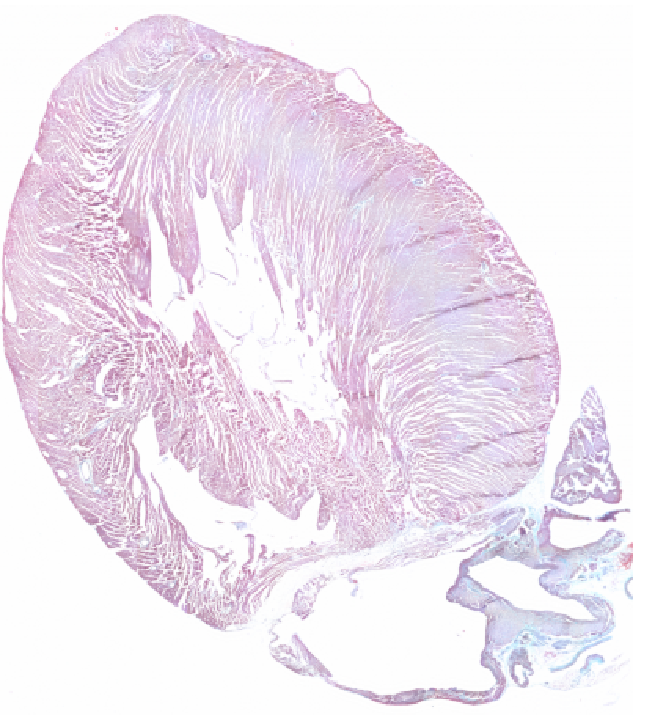
\includegraphics[height=0.365\textheight,type=pdf,ext=.pdf,read=.pdf]{Ch6/Figs/dummies/colour_perfect_slice}} \quad
    \subfigure[][image with transformational noise]{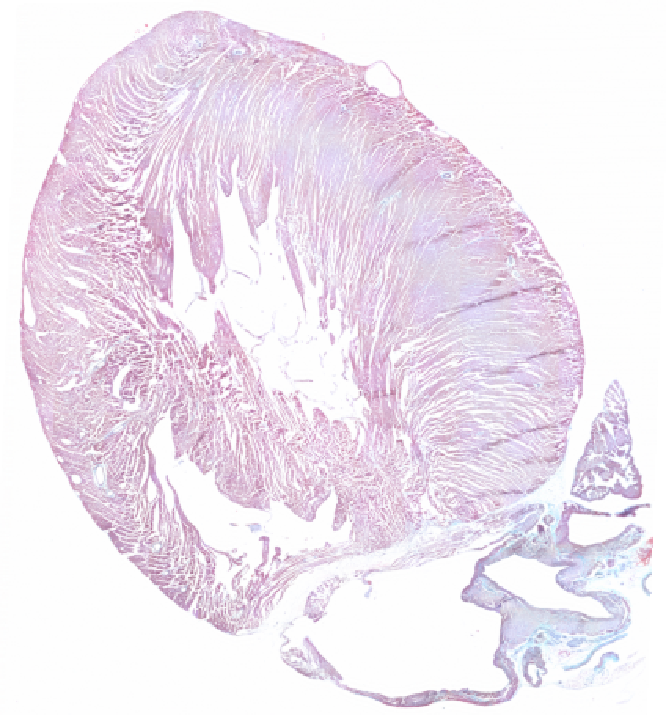
\includegraphics[height=0.365\textheight,type=pdf,ext=.pdf,read=.pdf]{Ch6/Figs/dummies/colour_noisy_slice}} \\
    \subfigure[][Red-blue channels of intensities]{\includegraphics[height=0.365\textheight,type=pdf,ext=.pdf,read=.pdf]{Ch6/Figs/dummies/colour_red_blue_diff}} \quad
    \subfigure[][squared differences in intensities]{\includegraphics[height=0.365\textheight,type=pdf,ext=.pdf,read=.pdf]{Ch6/Figs/dummies/colour_squared_diff}}
    \caption{Slice 200 from the Rat 28 dataset, the image used used for all test geometries. \textbf{(a)} shows the original image, whilst a small random affine transformation has been applied to \textbf{(b)}. \textbf{(c)} and \textbf{(d)} combine the two slices in two ways, in order to highlight their difference. The mean squared pixel intensity difference in \textbf{(d)} is 61.53.}
    \label{fig:original_displacement}
  \end{figure}
  
  % segmentation slice differences
  \begin{figure}[htbp]
    \centering
    \subfigure[][unperturbed image]{\includegraphics[height=0.365\textheight,type=pdf,ext=.pdf,read=.pdf]{Ch6/Figs/dummies/segmentation_perfect_slice}} \quad
    \subfigure[][image with transformational noise]{\includegraphics[height=0.365\textheight,type=pdf,ext=.pdf,read=.pdf]{Ch6/Figs/dummies/segmentation_noisy_slice}} \\
    \subfigure[][Red-blue channels of intensities]{\includegraphics[height=0.365\textheight,type=pdf,ext=.pdf,read=.pdf]{Ch6/Figs/dummies/segmentation_red_blue_diff}} \quad
    \subfigure[][squared differences in intensities]{\includegraphics[height=0.365\textheight,type=pdf,ext=.pdf,read=.pdf]{Ch6/Figs/dummies/segmentation_squared_diff}}
    \caption{A manual segmentation of the same slice from Figure~\ref{fig:original_displacement}, with the same perturbation applied. The noise in the squared intensity differences in Figure~\ref{fig:original_displacement}~\textbf{(d)} are no longer present. This leads to a much smoother cost function, with much fewer local minima, and thus a more reliable registration. The improvement is reflected in the lower mean squared pixel intensity difference in \textbf{(d)} of 12.93.}
    \label{fig:segmented_displacement}
  \end{figure}
  
  The process of registration between slices, of obtaining the values $\mathbf{\Delta T}_{i,i+1}^n$, is orthogonal to and separate from the calculation of the diffusion transforms $\mathbf{\Delta T}_i^{n,n+1}$ and subsequent adjustment of each slice transform $\mathbf{T}_i^{n+1}$. The first attempt to test the algorithm used the original heart slice image shown in Figure~\ref{fig:original_displacement}. Although the algorithm was reliably stable in smoothing the small amplitudes of noise it was designed to correct for, it was found that much larger perturbations could be damped by the algorithm, limited only by the success of the individual registrations. All registrations were therefore performed using the manual segmentations shown in Figure~\ref{fig:segmented_displacement}, with which much larger displacements could be corrected. As will be seen, cross-sections were then reconstructed from the original images, to show the effects of correction on the fine detail of the tissue, whilst clean volume isosurfaces were constructed from the segmentation.
  
  % straight
  \begin{figure}[htbp]
    \centering
    % filename format: cross_section_200_alpha0.4_ITERATION_DIMENSION_SLICE
    \subfigure[][with noise (0 iterations)]{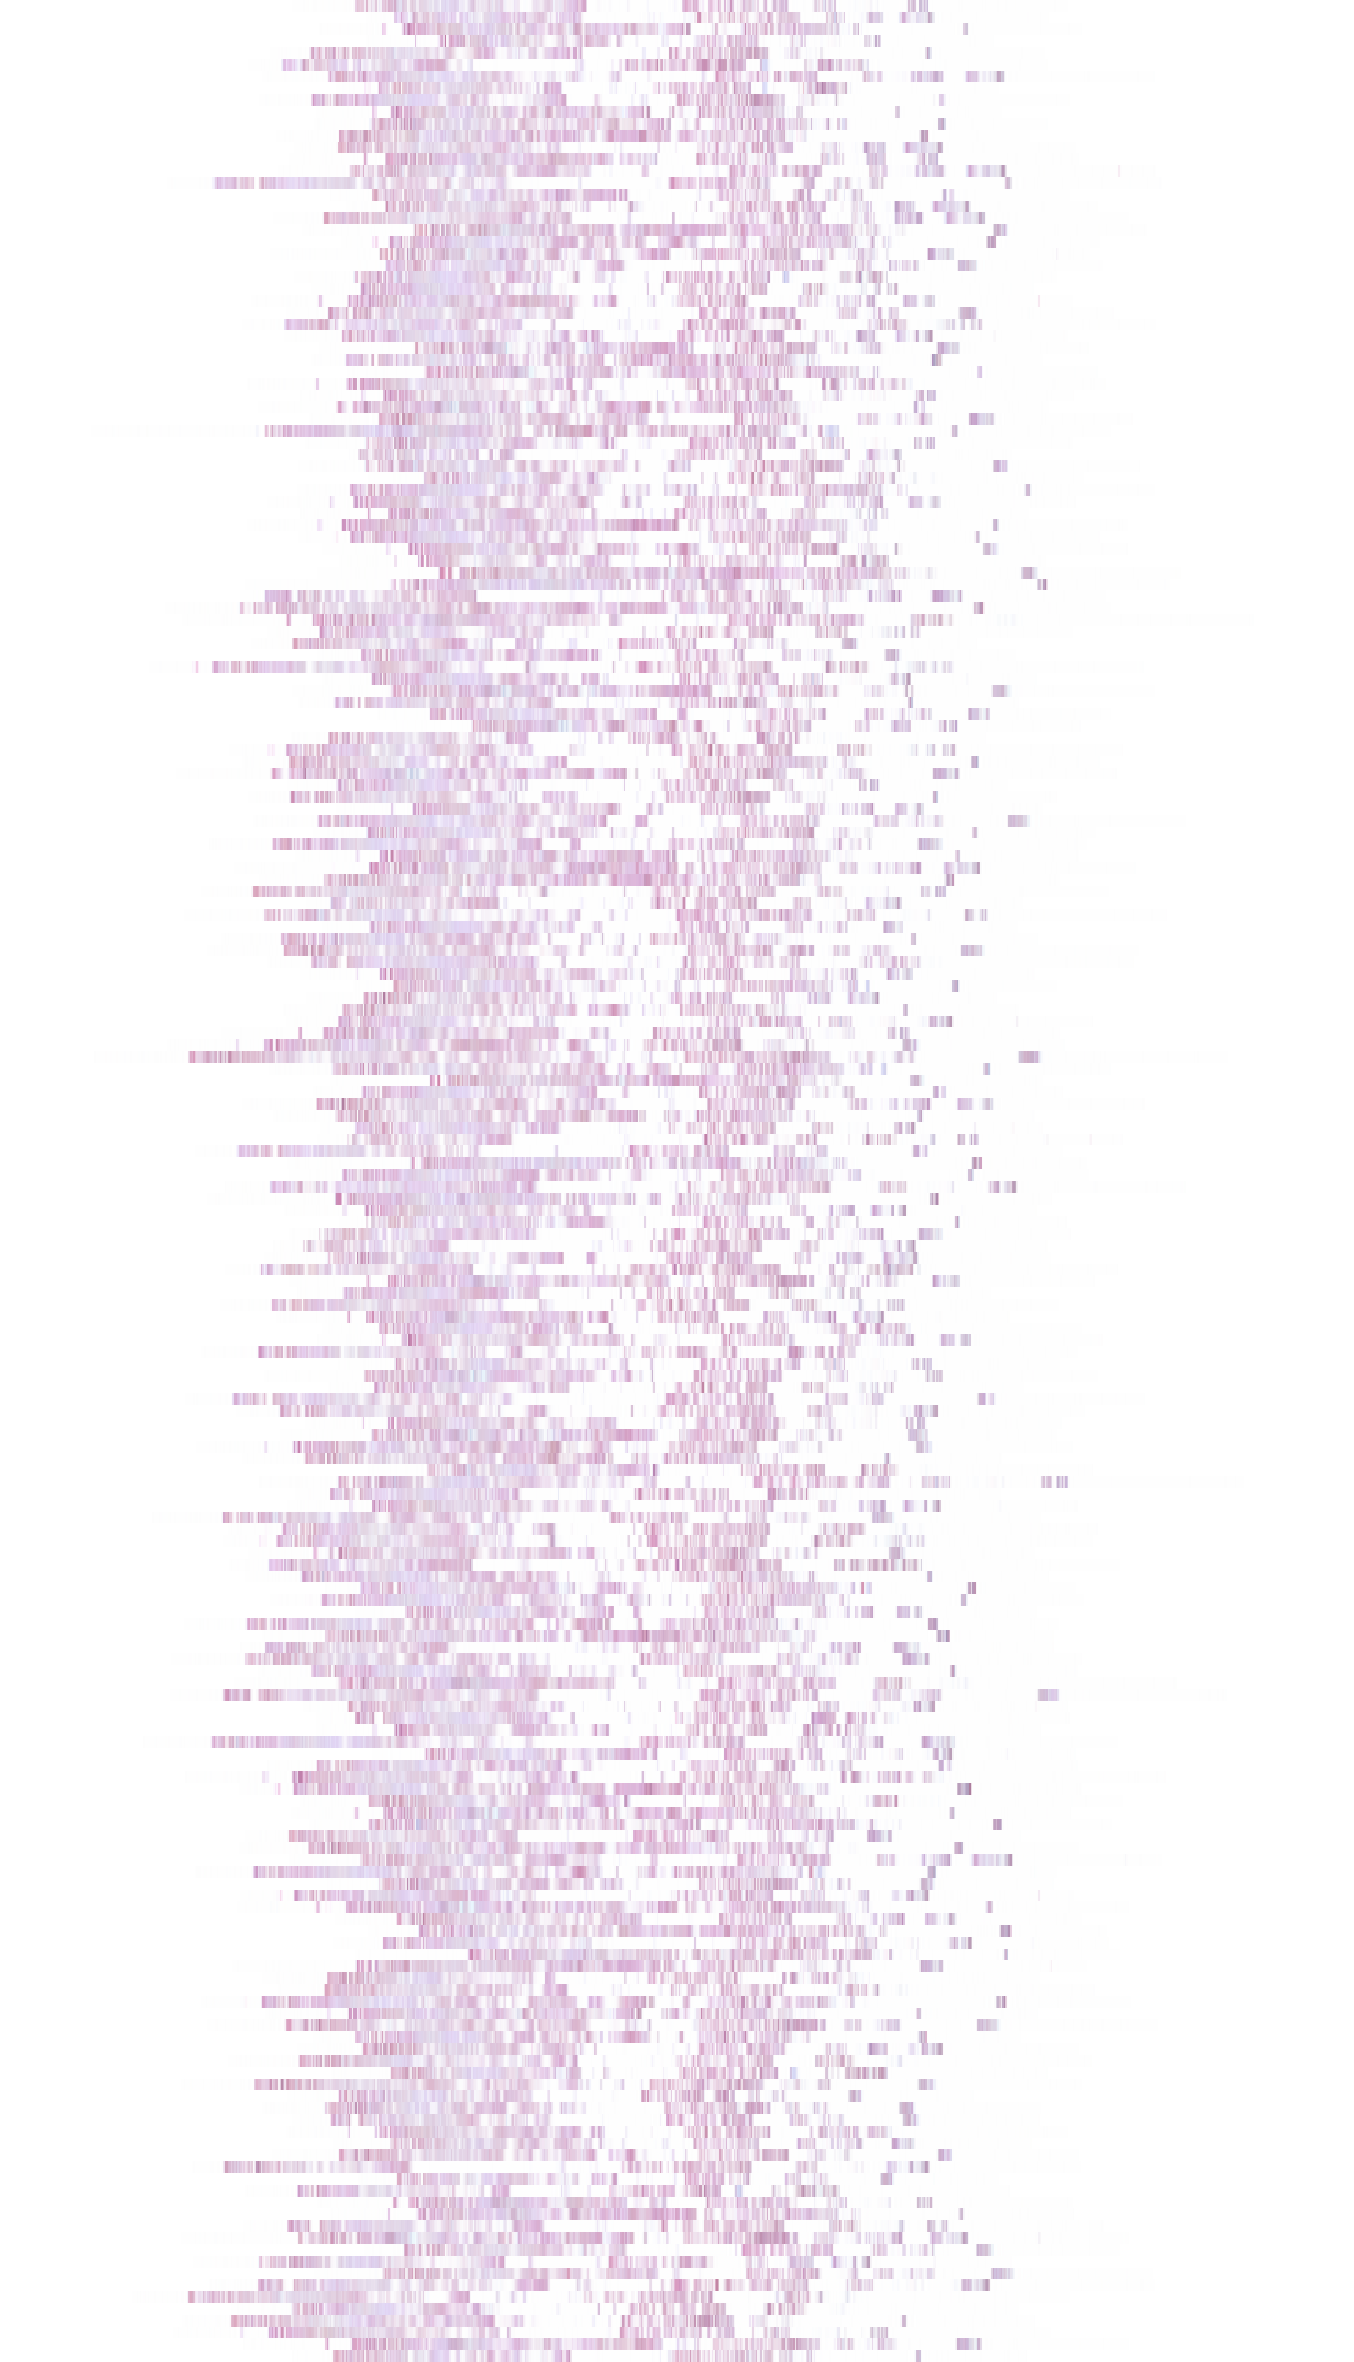
\includegraphics[height=0.4\textheight,type=pdf,ext=.pdf,read=.pdf]{Ch6/Figs/dummies/cross_section_200_alpha0.4_0_0_352}\label{fig:subfig1}}
    \subfigure[][1 iteration]{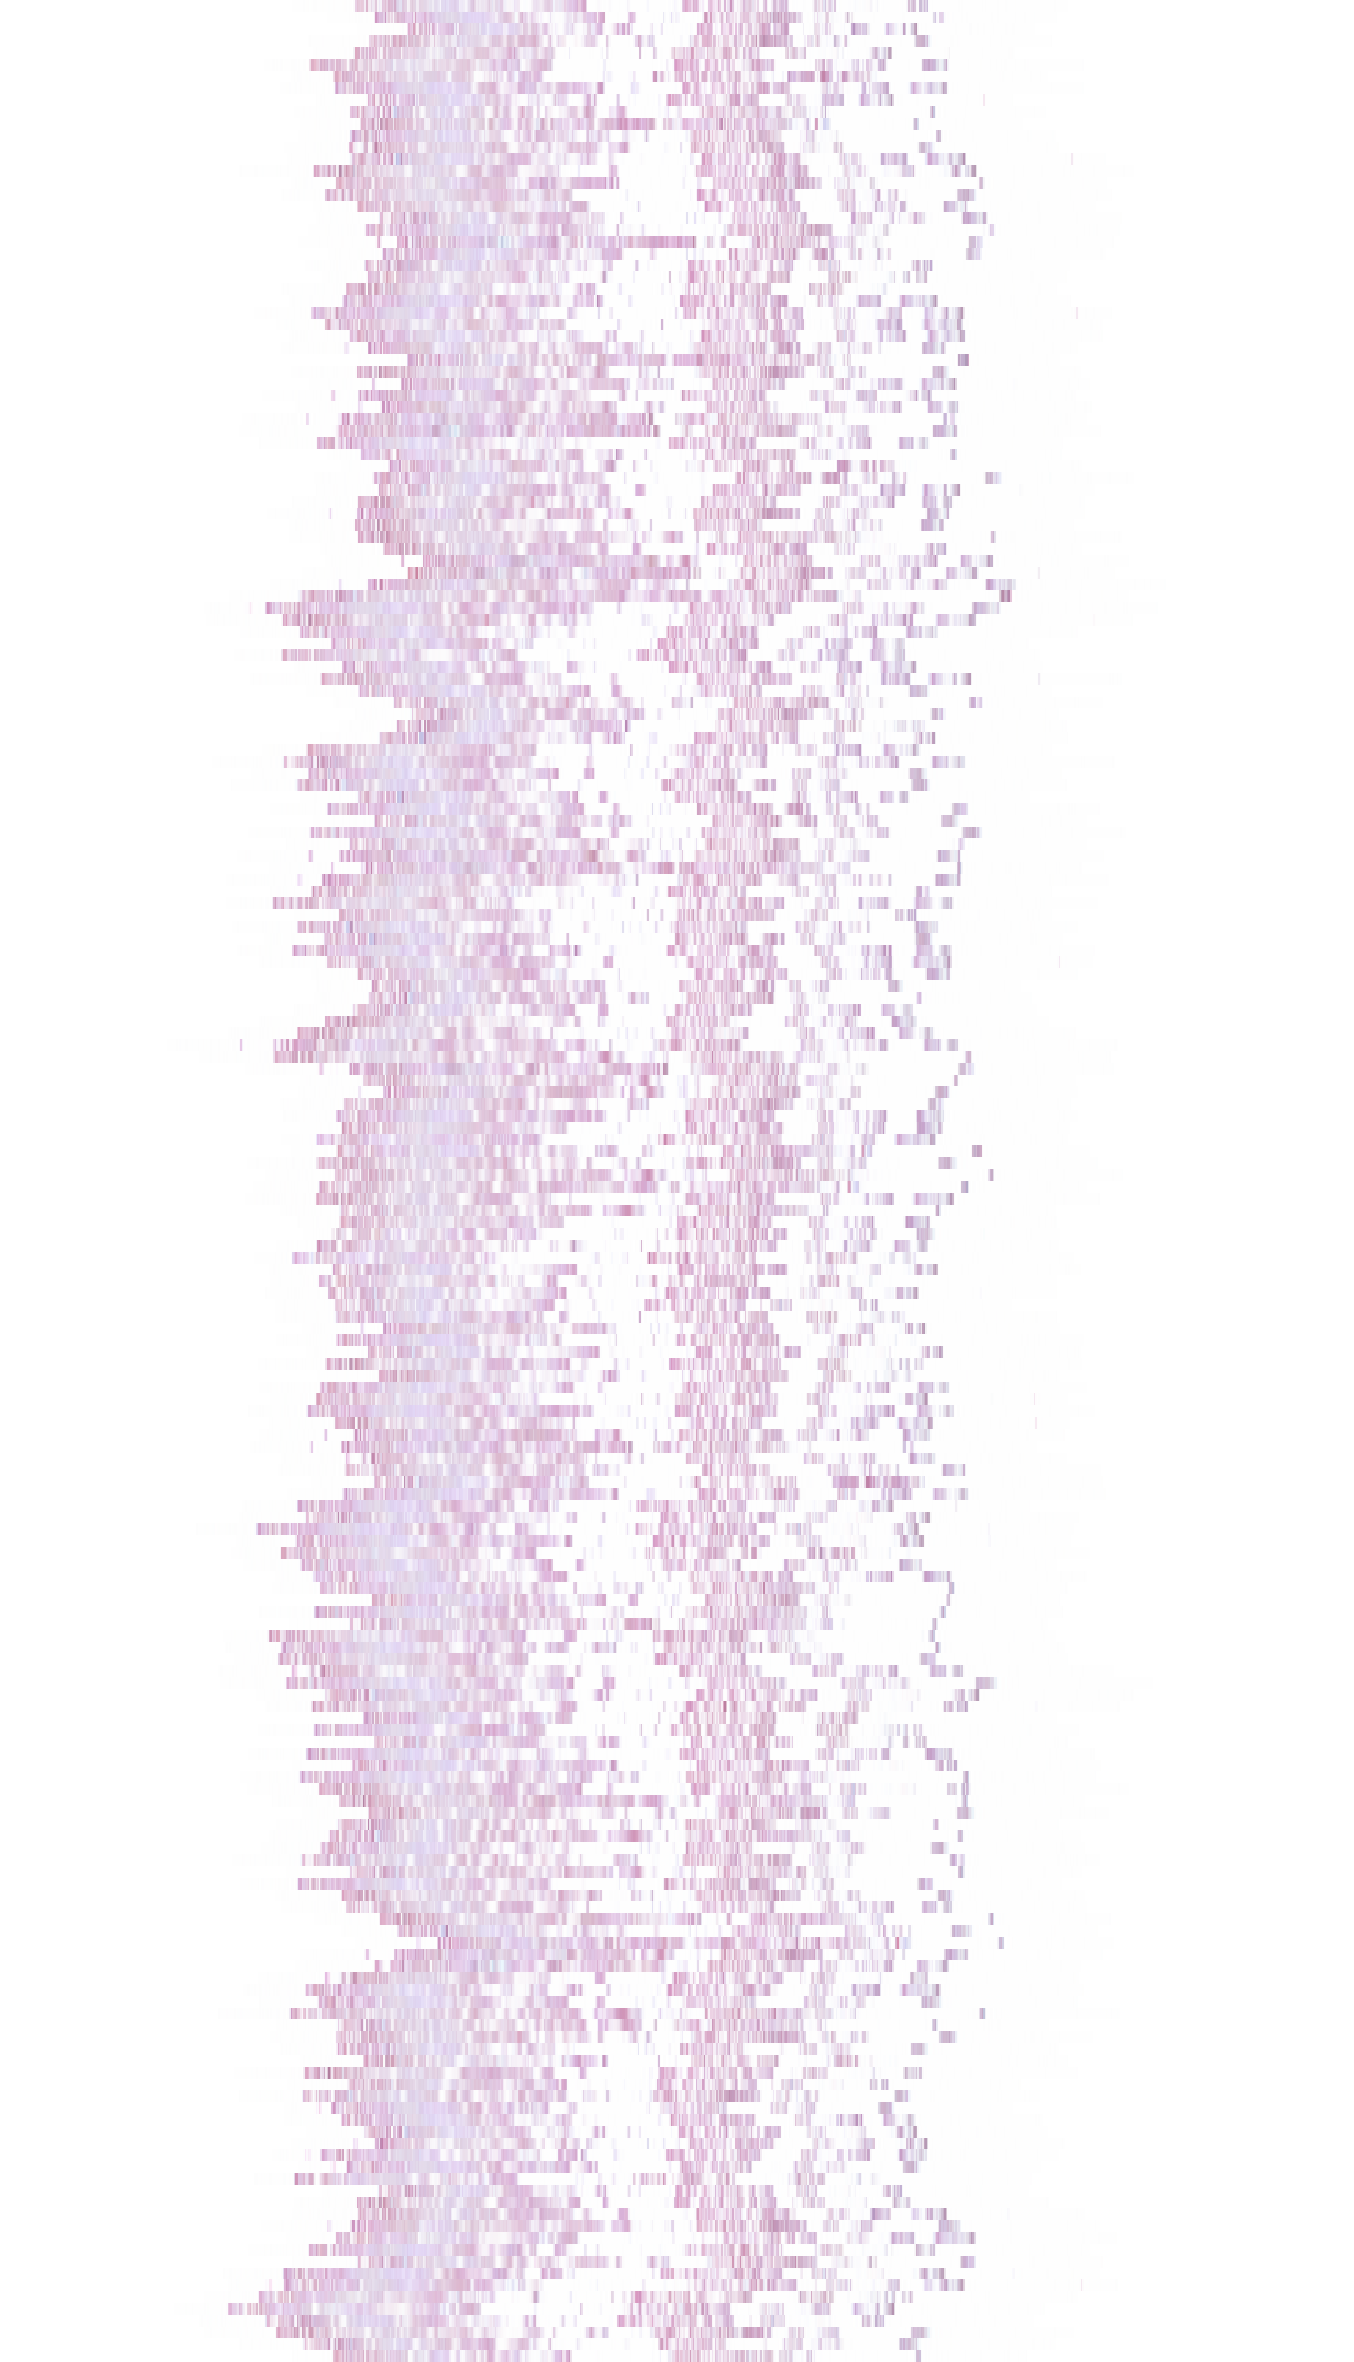
\includegraphics[height=0.4\textheight,type=pdf,ext=.pdf,read=.pdf]{Ch6/Figs/dummies/cross_section_200_alpha0.4_1_0_352}\label{fig:subfig2}}
    \subfigure[][3 iterations]{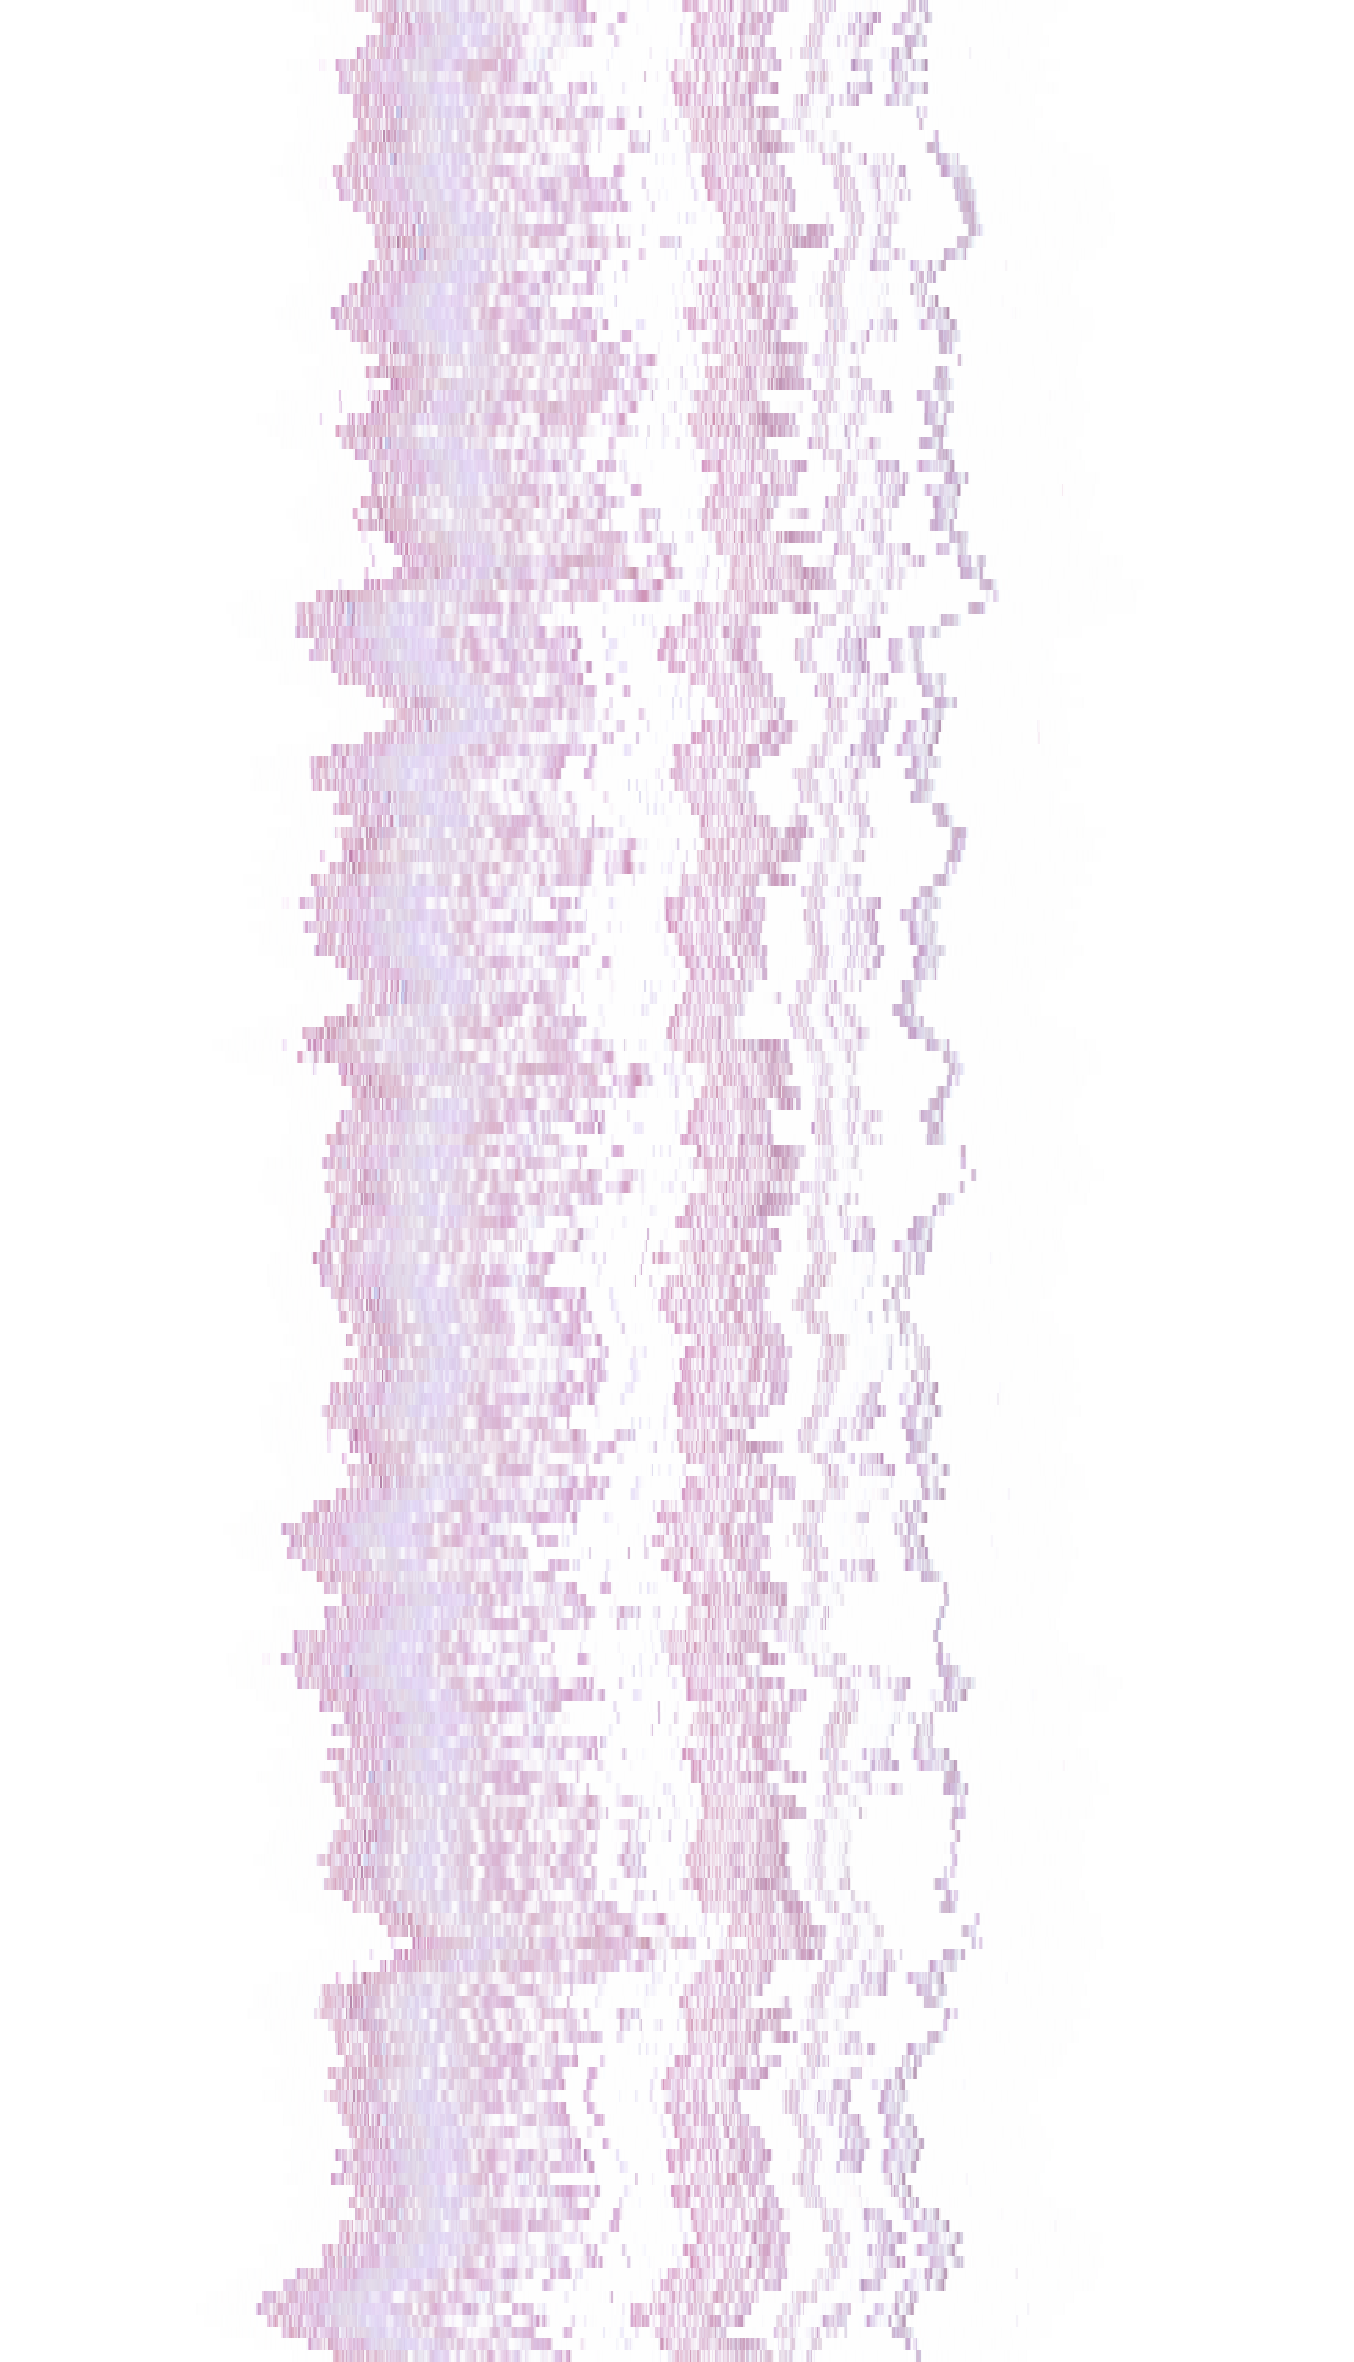
\includegraphics[height=0.4\textheight,type=pdf,ext=.pdf,read=.pdf]{Ch6/Figs/dummies/cross_section_200_alpha0.4_3_0_352}\label{fig:subfig3}}
    \subfigure[][8 iterations]{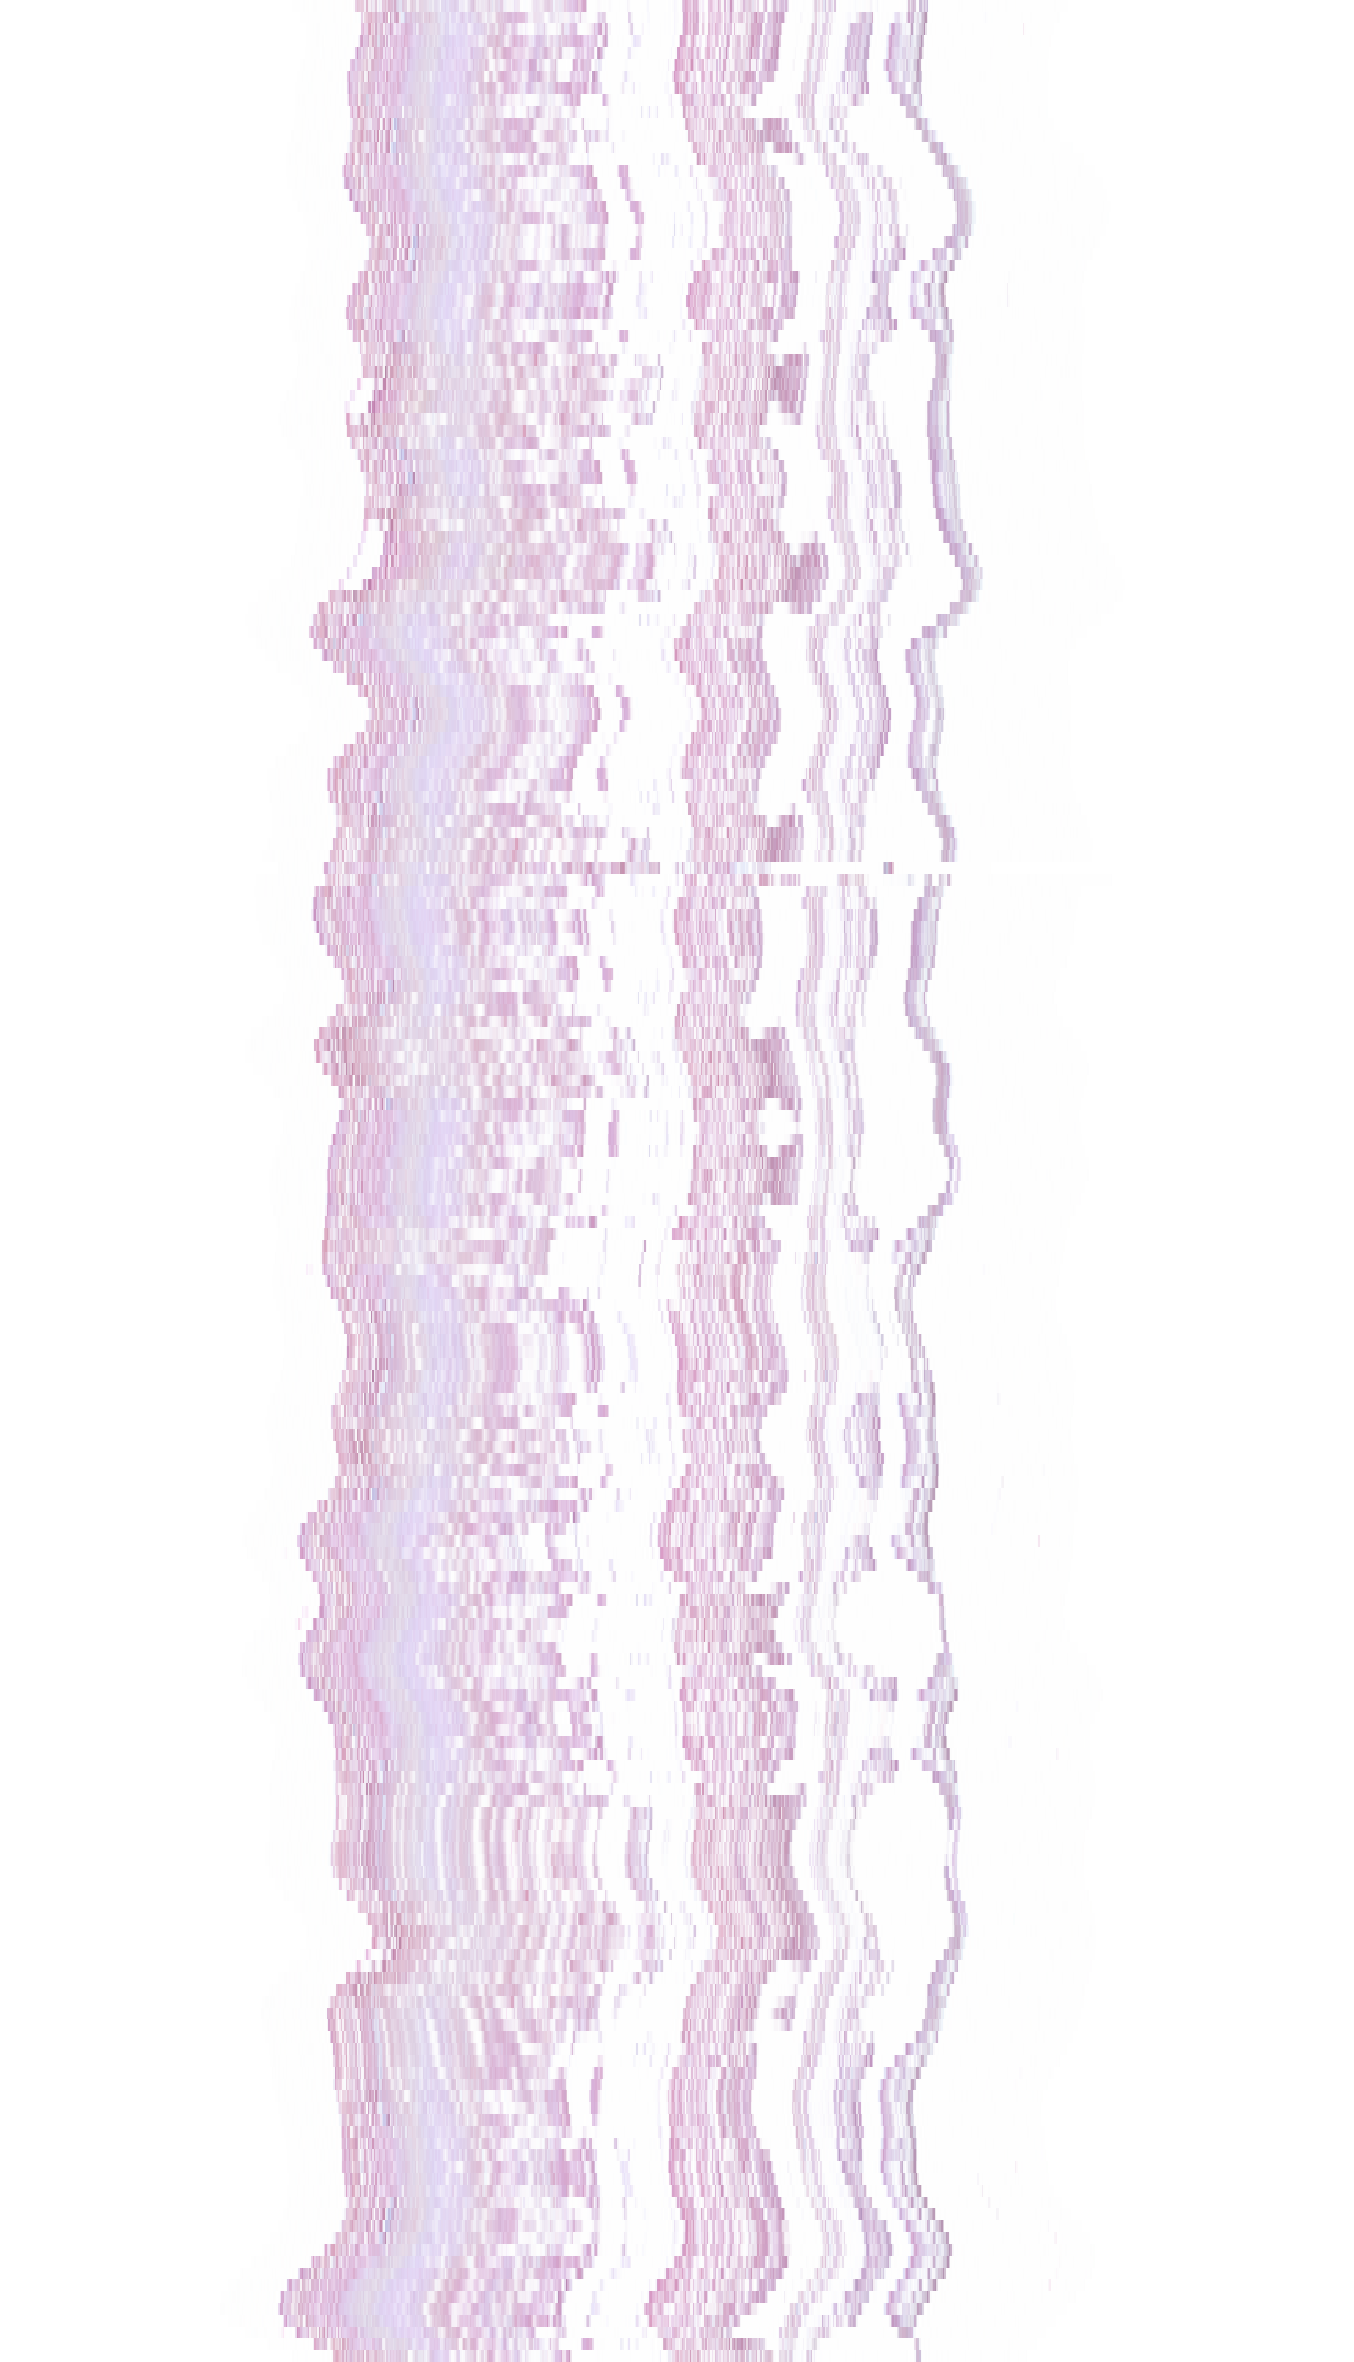
\includegraphics[height=0.4\textheight,type=pdf,ext=.pdf,read=.pdf]{Ch6/Figs/dummies/cross_section_200_alpha0.4_8_0_352}\label{fig:subfig4}}
    \subfigure[][20 iterations]{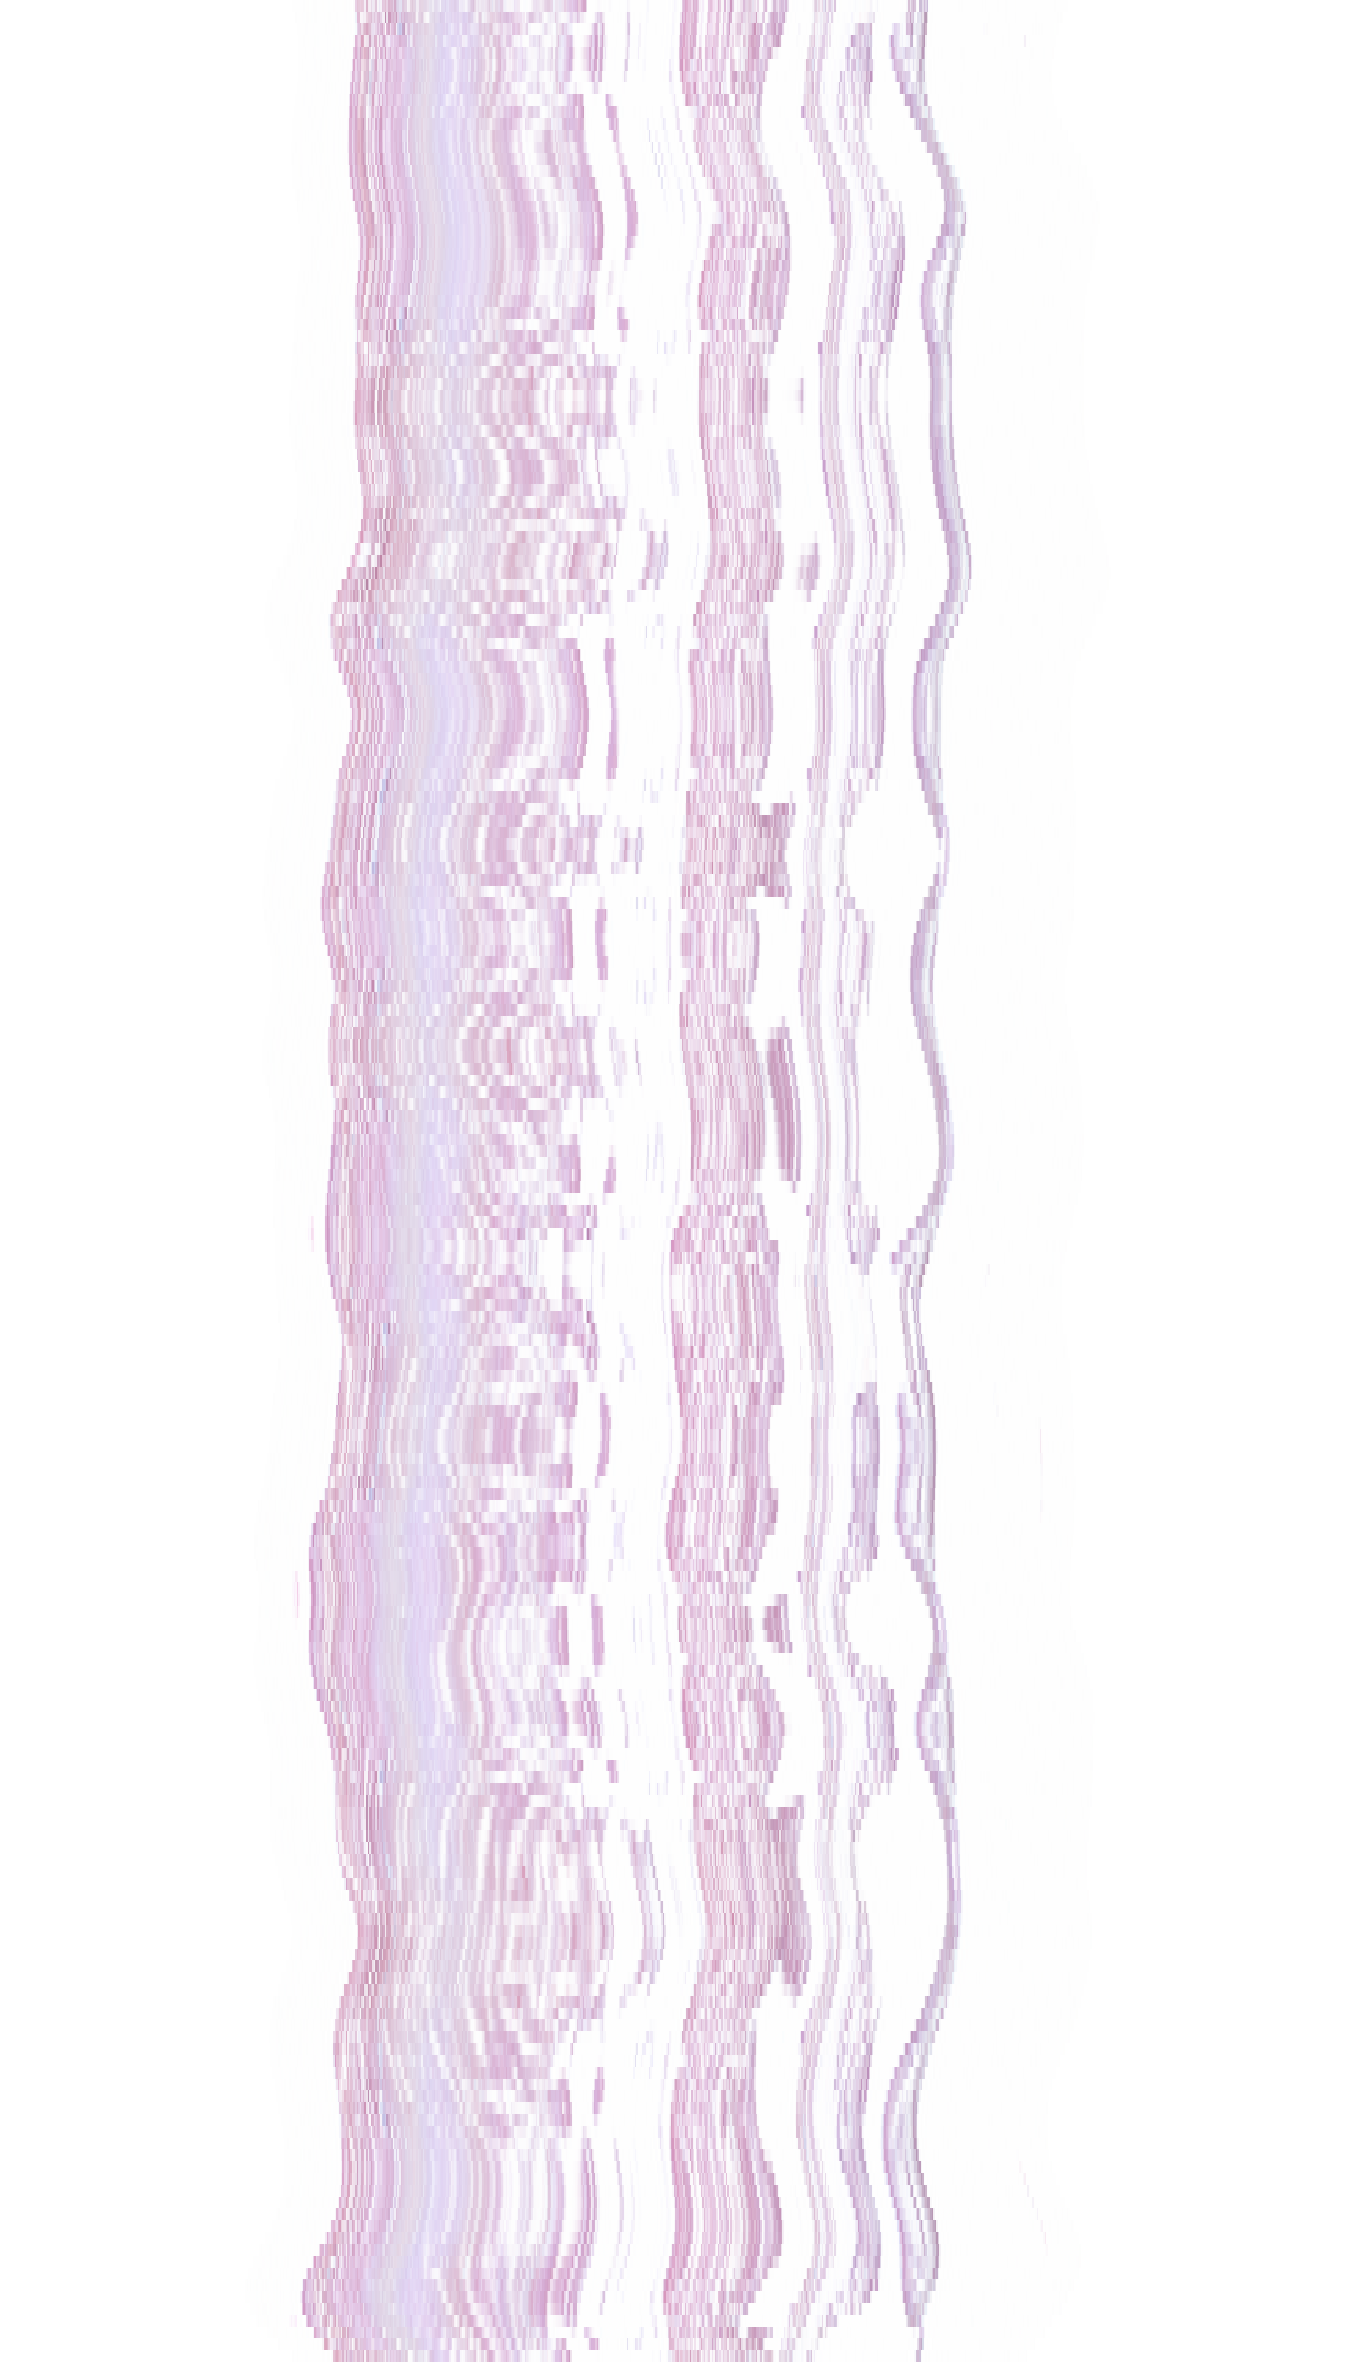
\includegraphics[height=0.4\textheight,type=pdf,ext=.pdf,read=.pdf]{Ch6/Figs/dummies/cross_section_200_alpha0.4_20_0_352}\label{fig:subfig4}}
    % filename format: cross_section_perfect_200_alpha0.4_DIMENSION_SLICE
    \subfigure[][without noise]{
\includegraphics[height=0.4\textheight,type=pdf,ext=.pdf,read=.pdf]{Ch6/Figs/dummies/cross_section_perfect_200_alpha0.4_0_352}}
    \caption{Cross-sections of the straight volume, perpendicular to the x-axis.}
    \label{fig:cross_section_0}
  \end{figure}
  
  \begin{figure}[htbp]
    \centering
    \subfigure[][0 iterations]{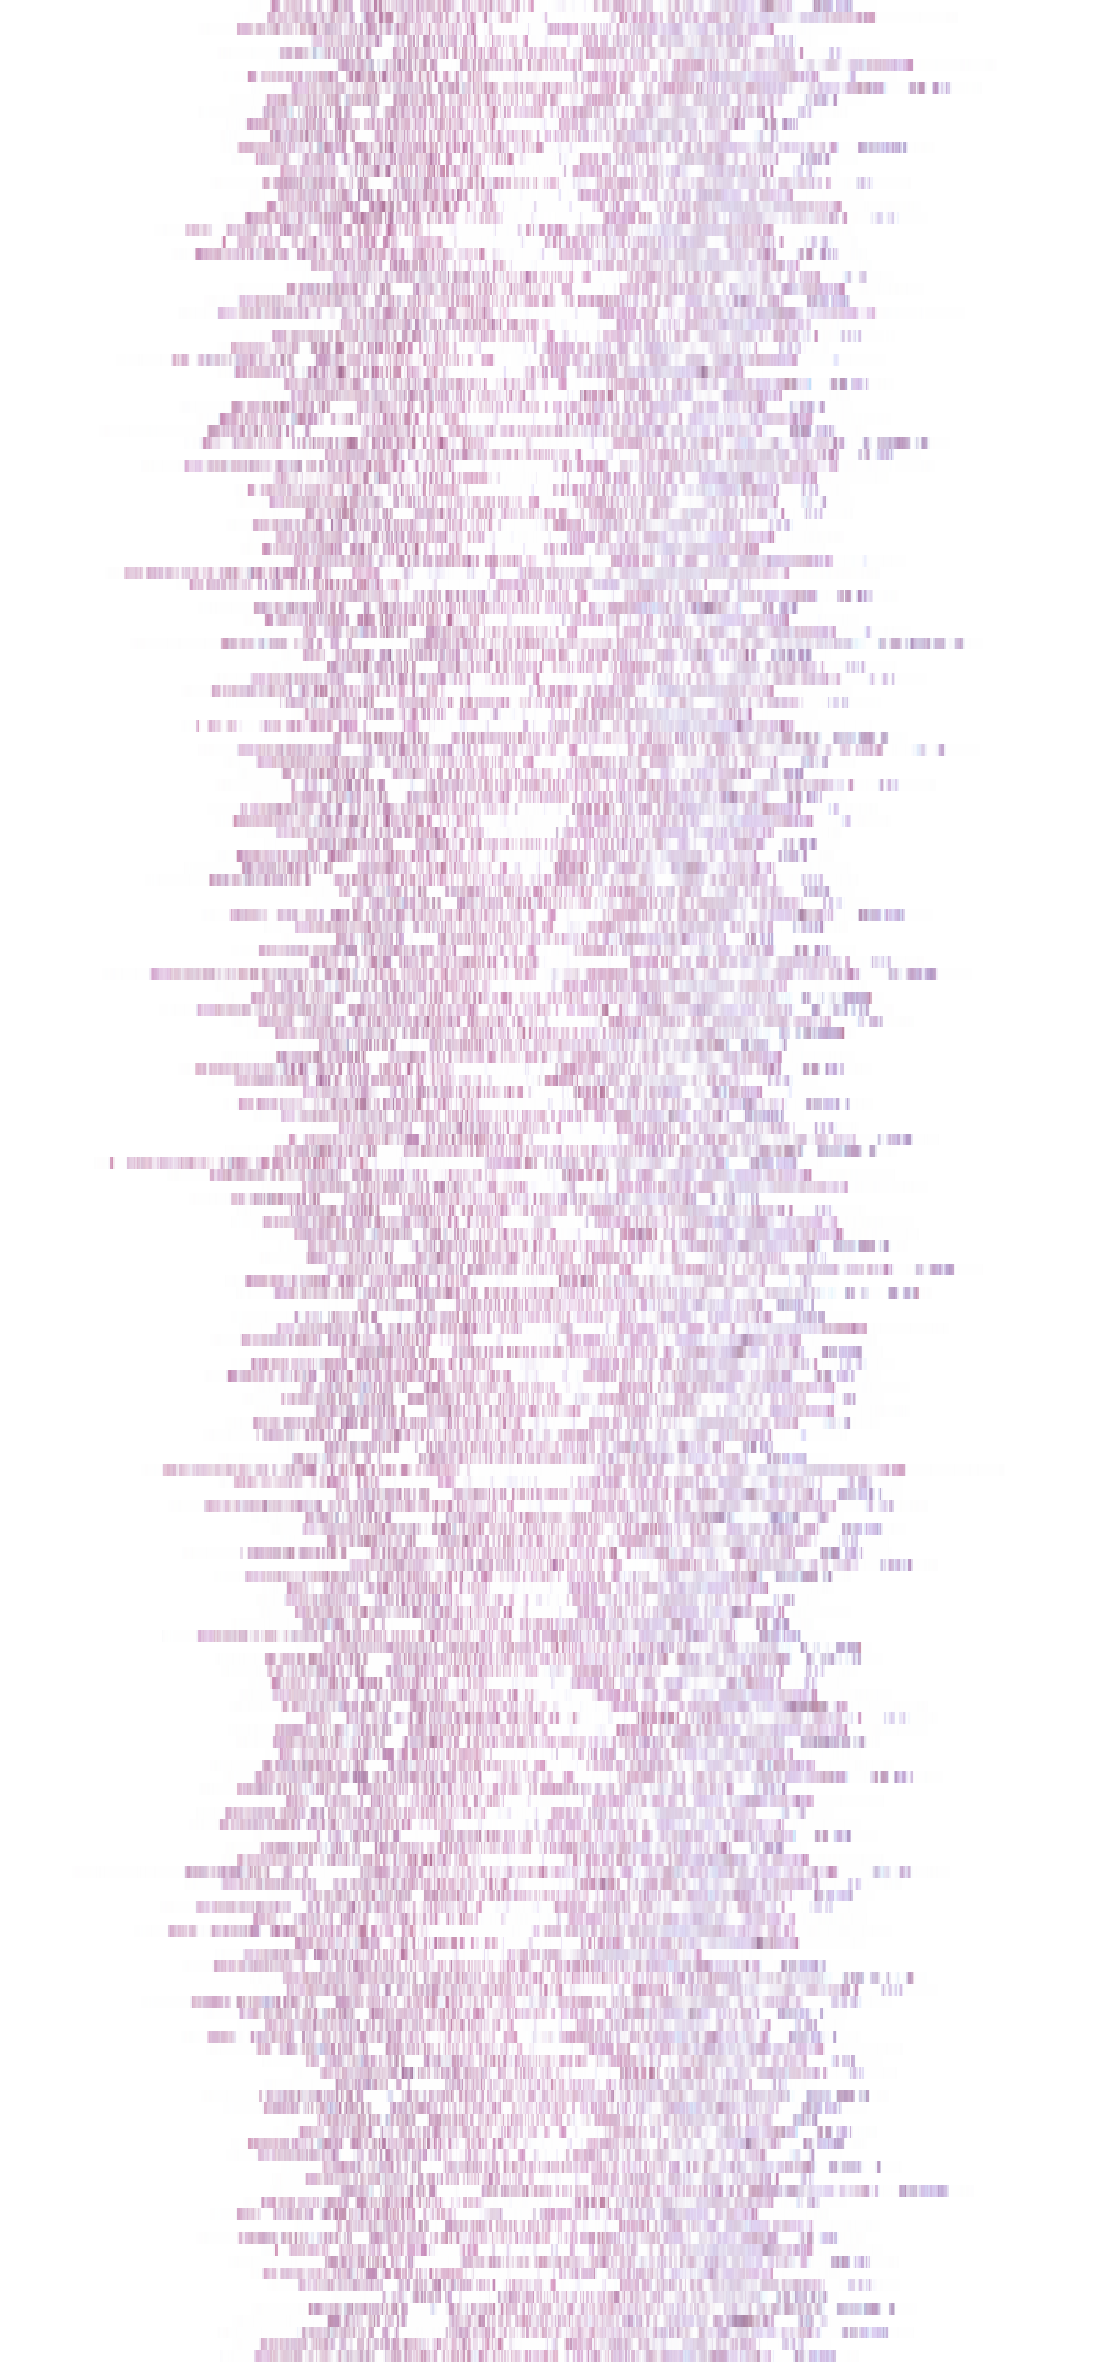
\includegraphics[height=0.4\textheight,type=pdf,ext=.pdf,read=.pdf]{Ch6/Figs/dummies/cross_section_200_alpha0.4_0_1_431}}
    \subfigure[][1 iteration]{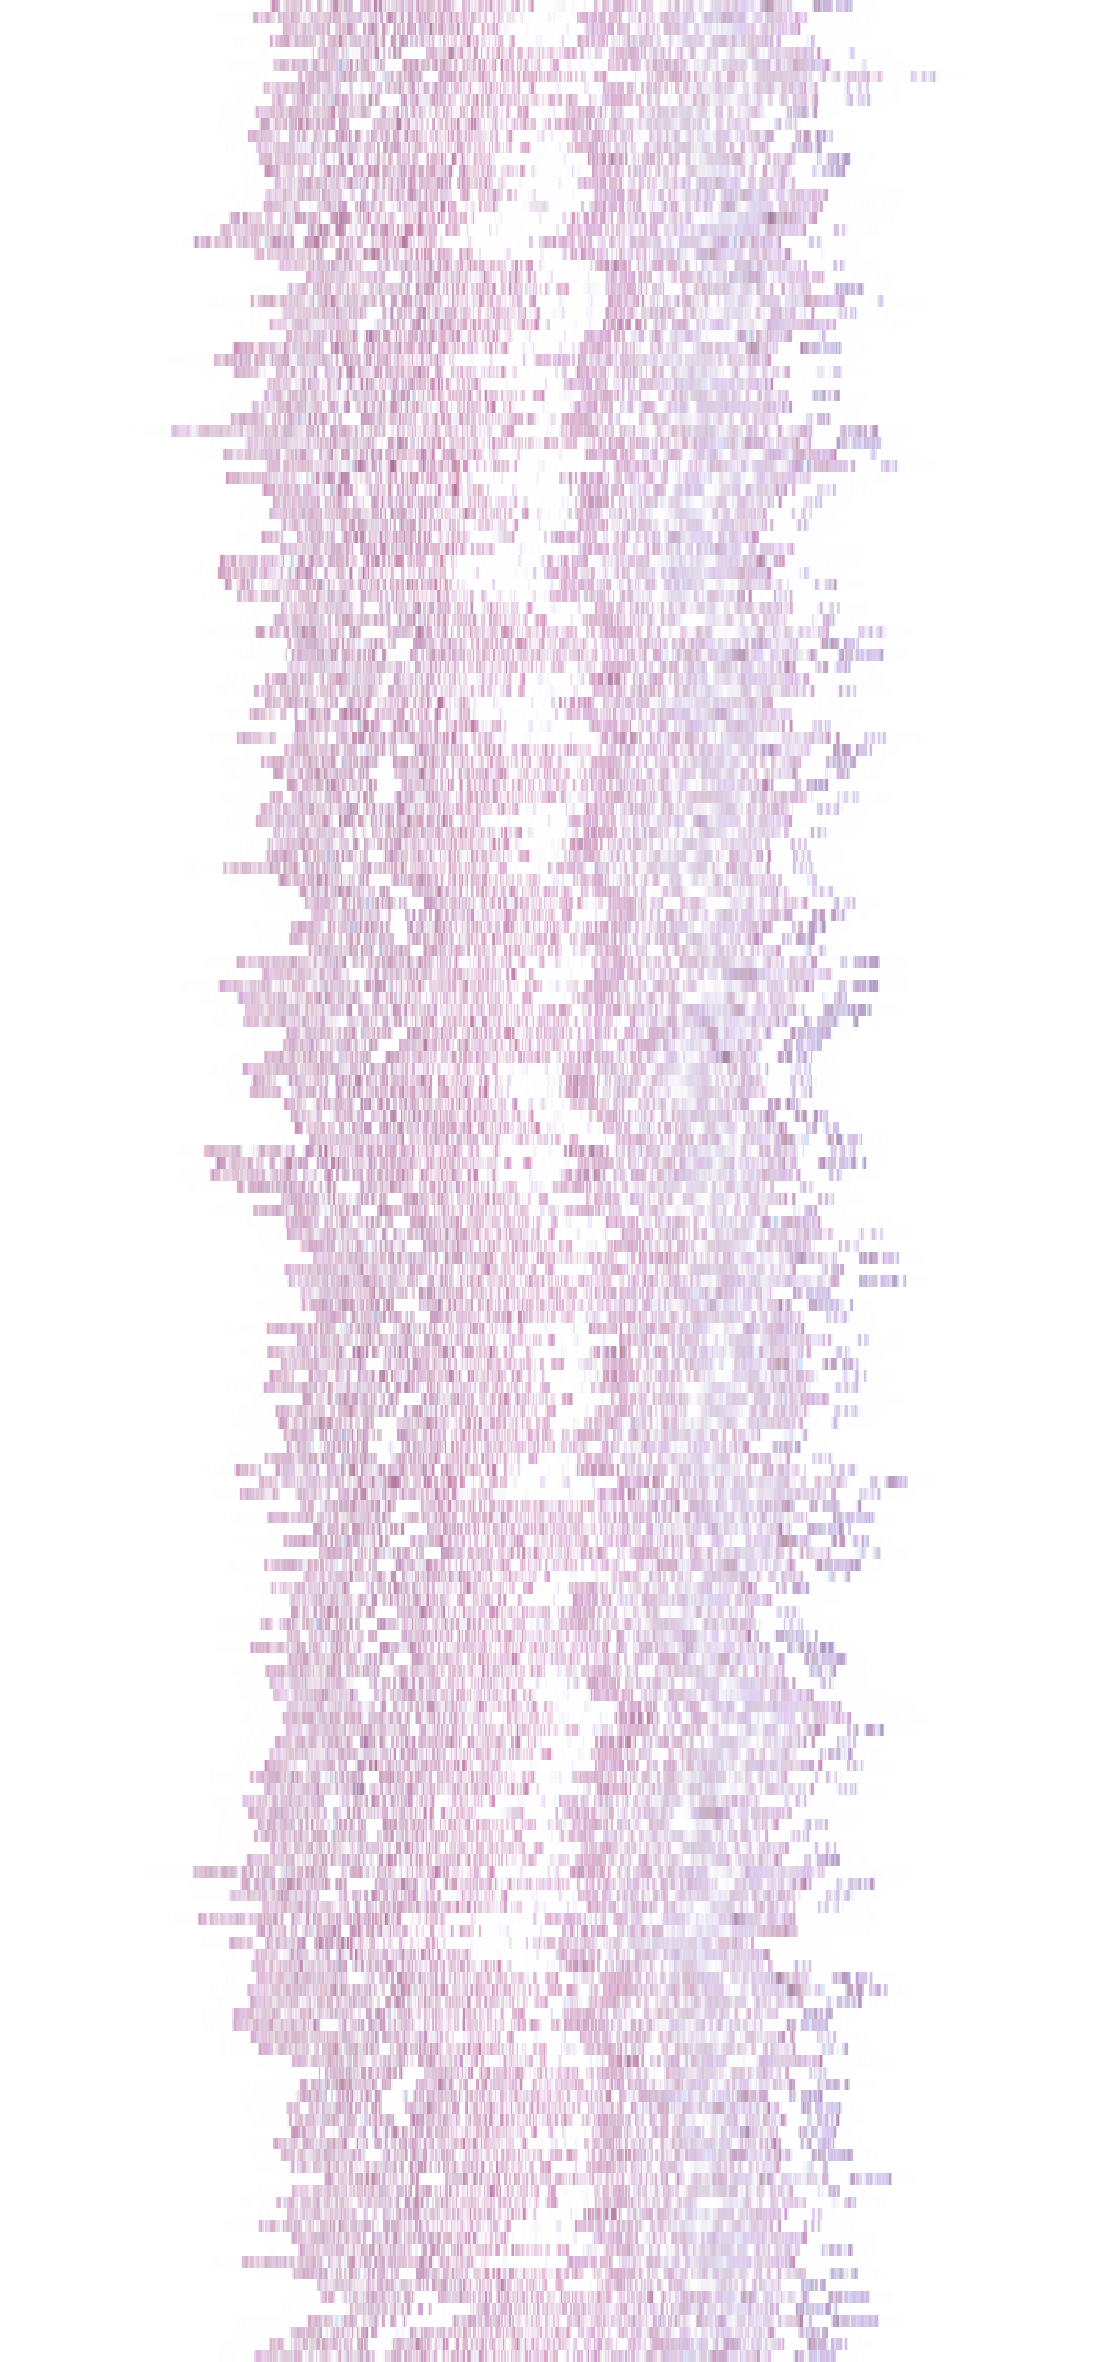
\includegraphics[height=0.4\textheight,type=pdf,ext=.pdf,read=.pdf]{Ch6/Figs/dummies/cross_section_200_alpha0.4_1_1_431}}
    \subfigure[][3 iterations]{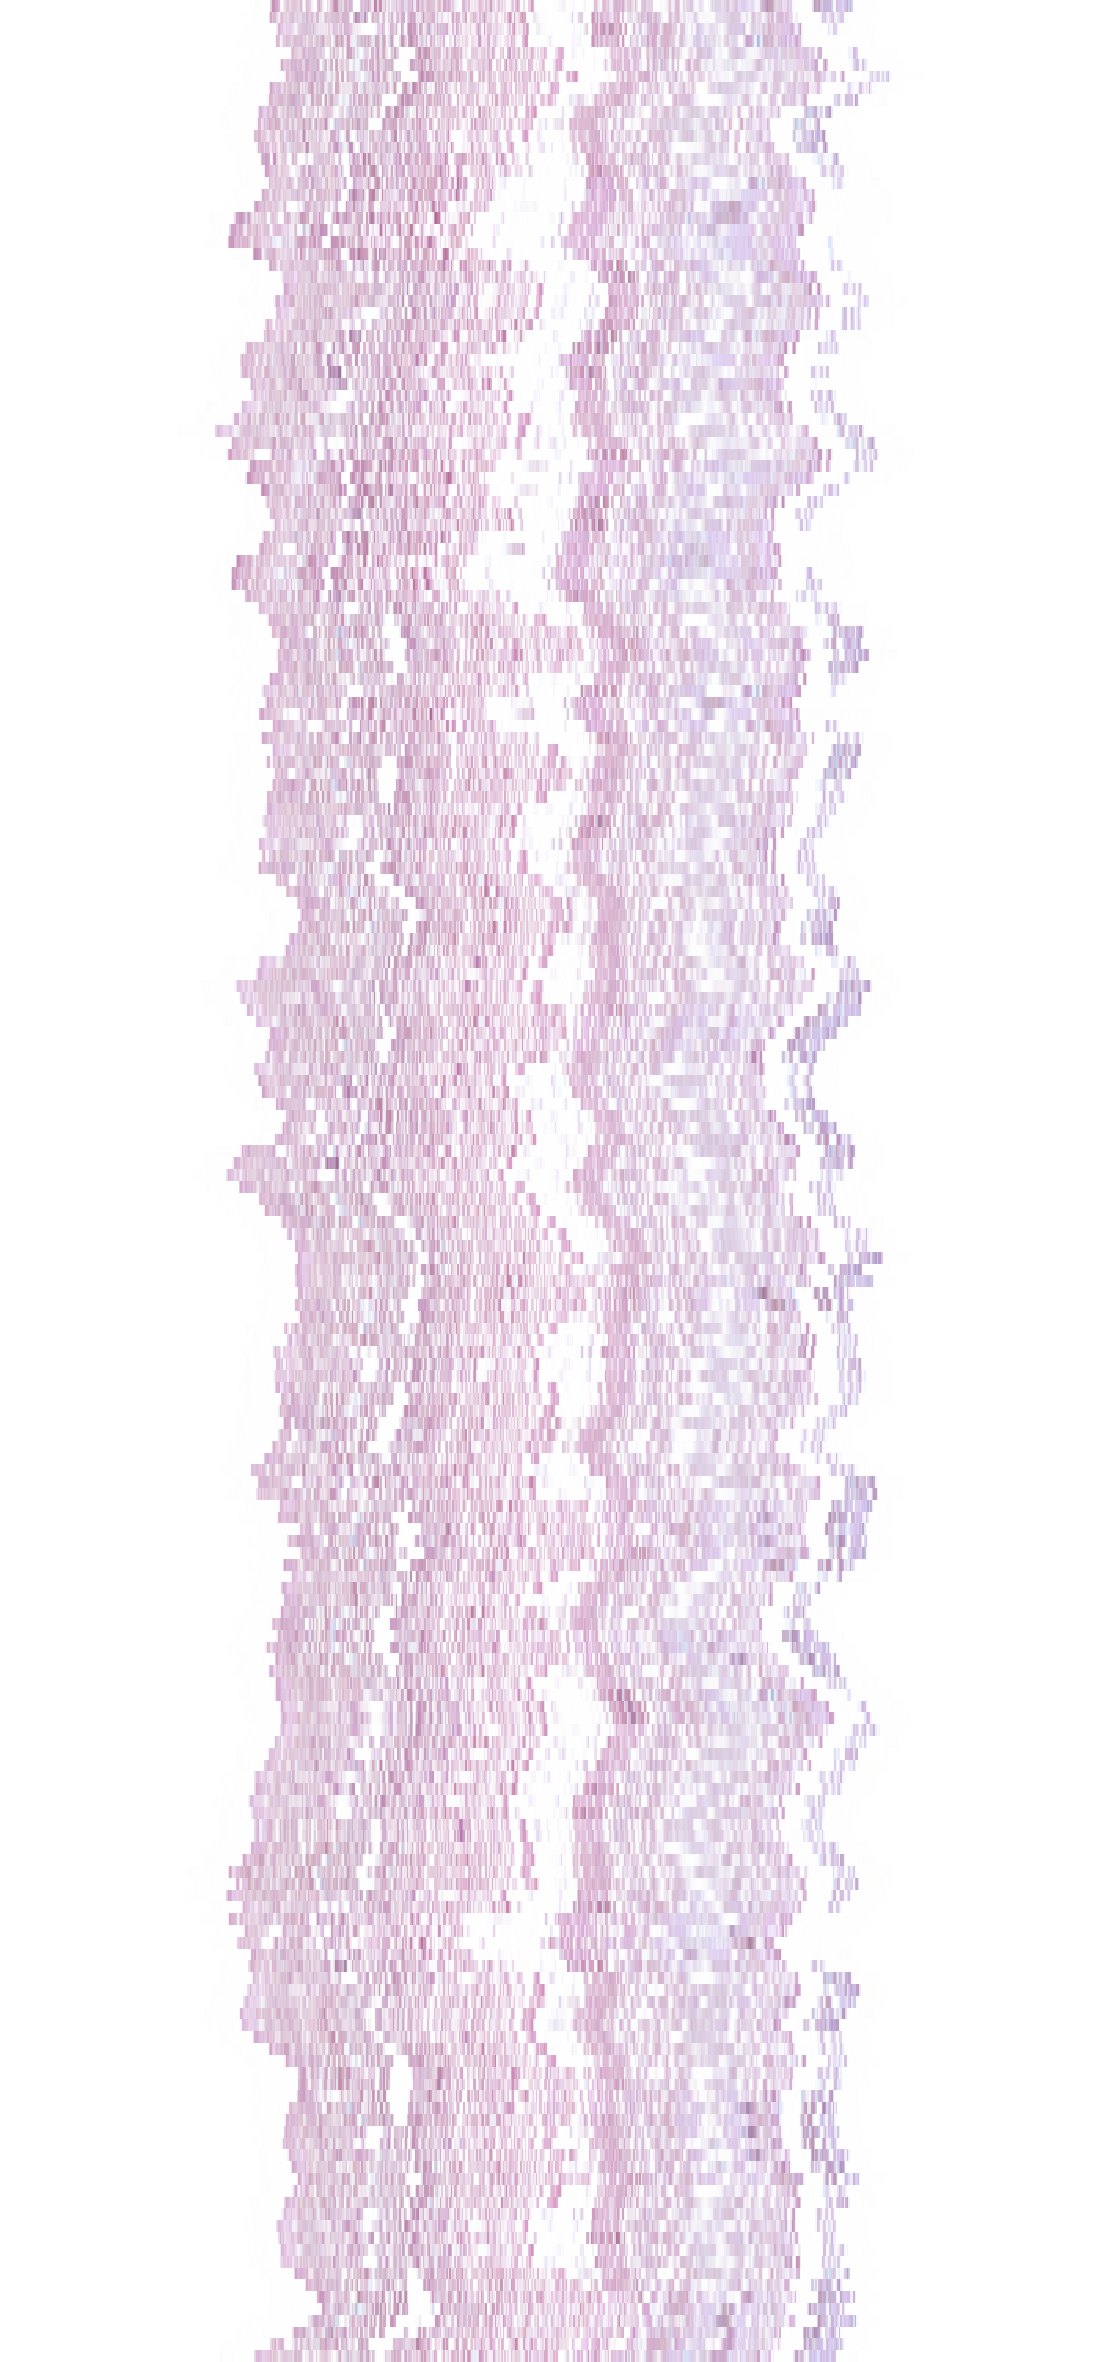
\includegraphics[height=0.4\textheight,type=pdf,ext=.pdf,read=.pdf]{Ch6/Figs/dummies/cross_section_200_alpha0.4_3_1_431}}
    \subfigure[][8 iterations]{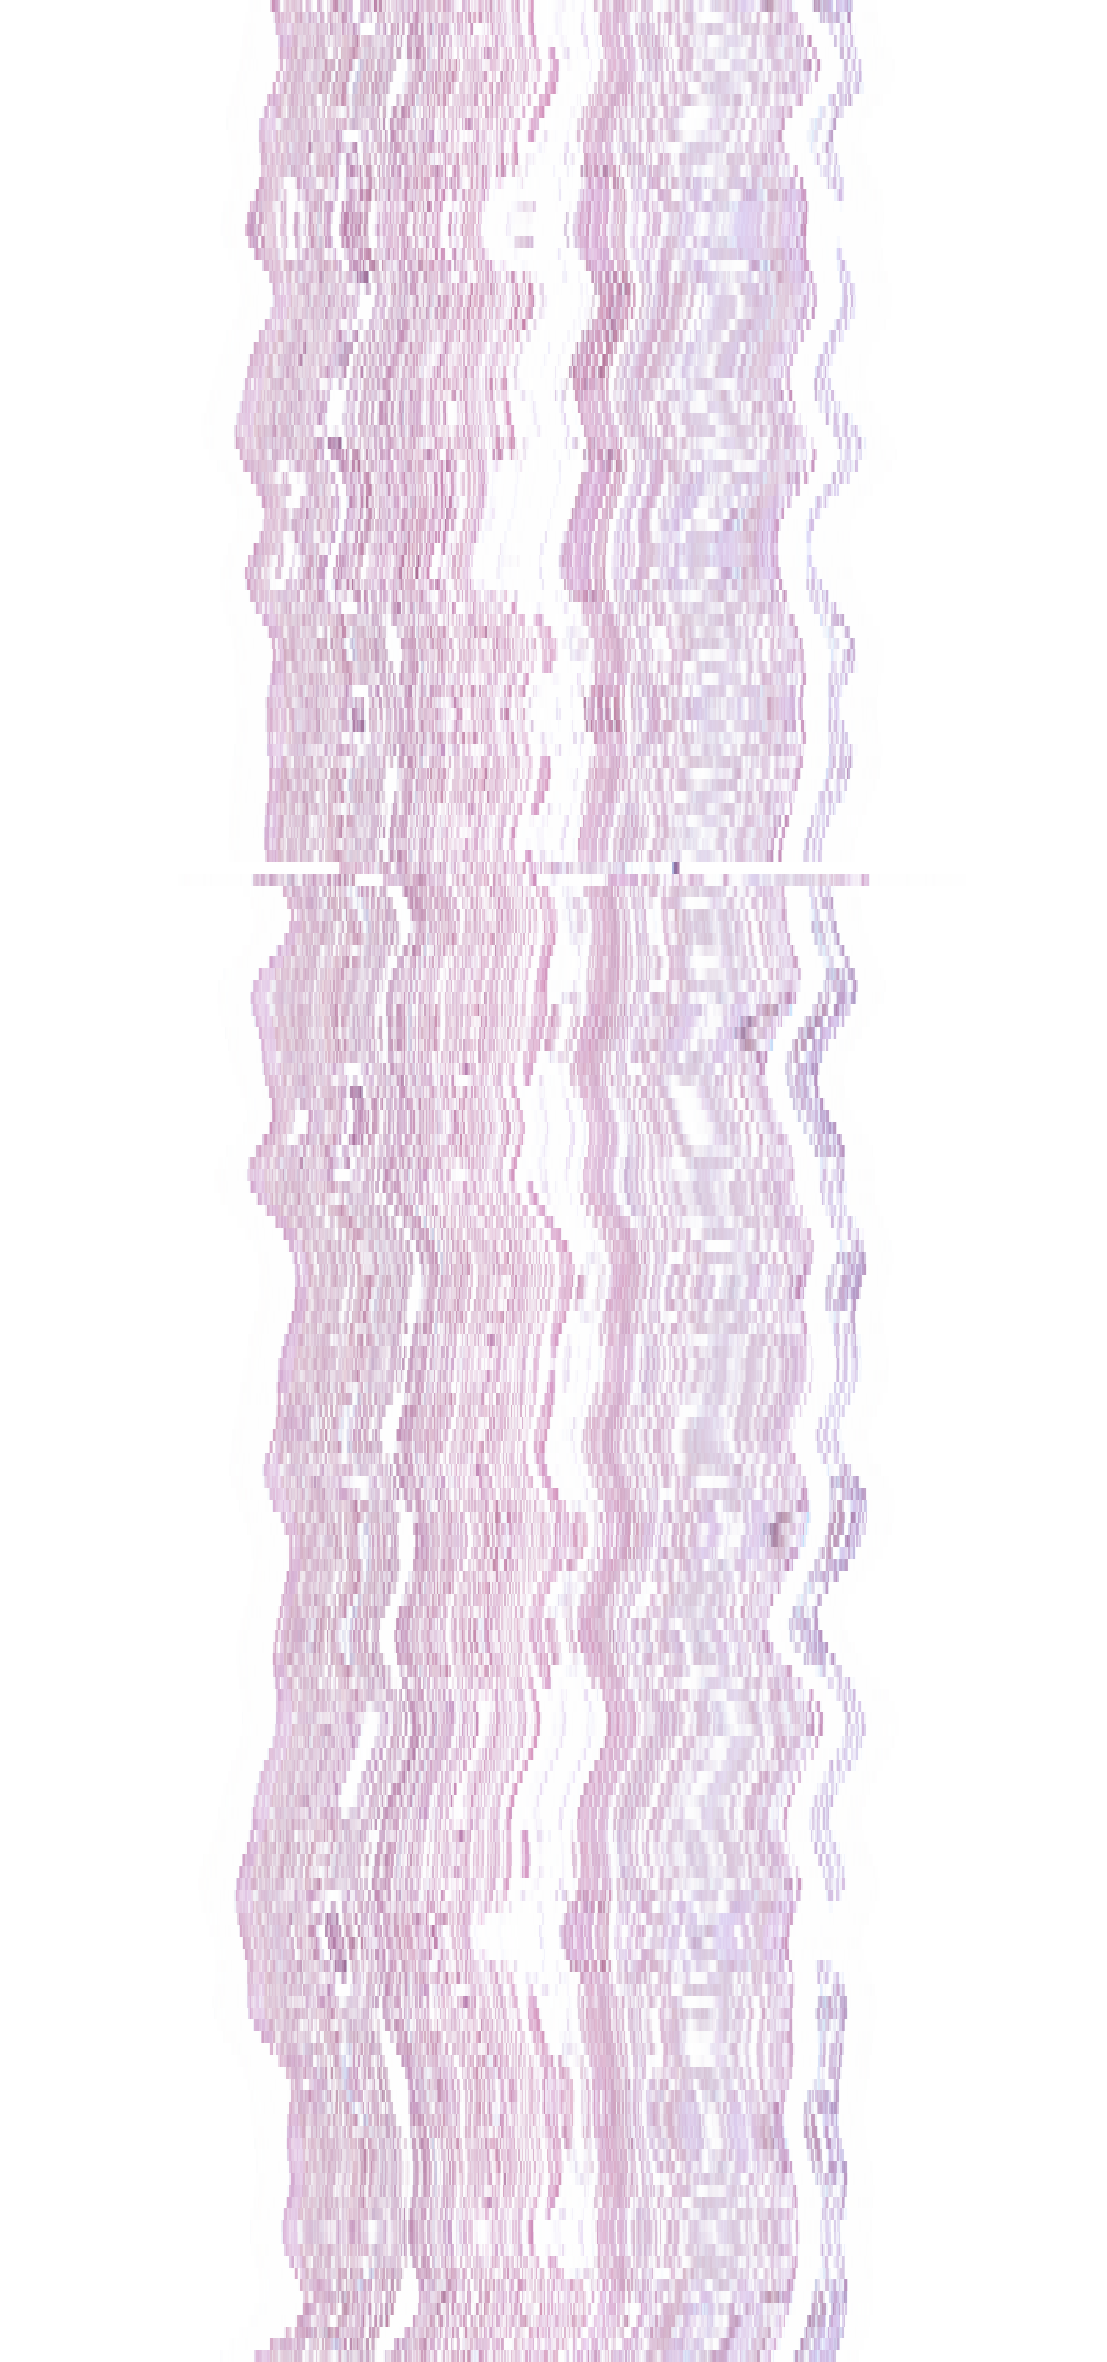
\includegraphics[height=0.4\textheight,type=pdf,ext=.pdf,read=.pdf]{Ch6/Figs/dummies/cross_section_200_alpha0.4_8_1_431}}
    \subfigure[][20 iterations]{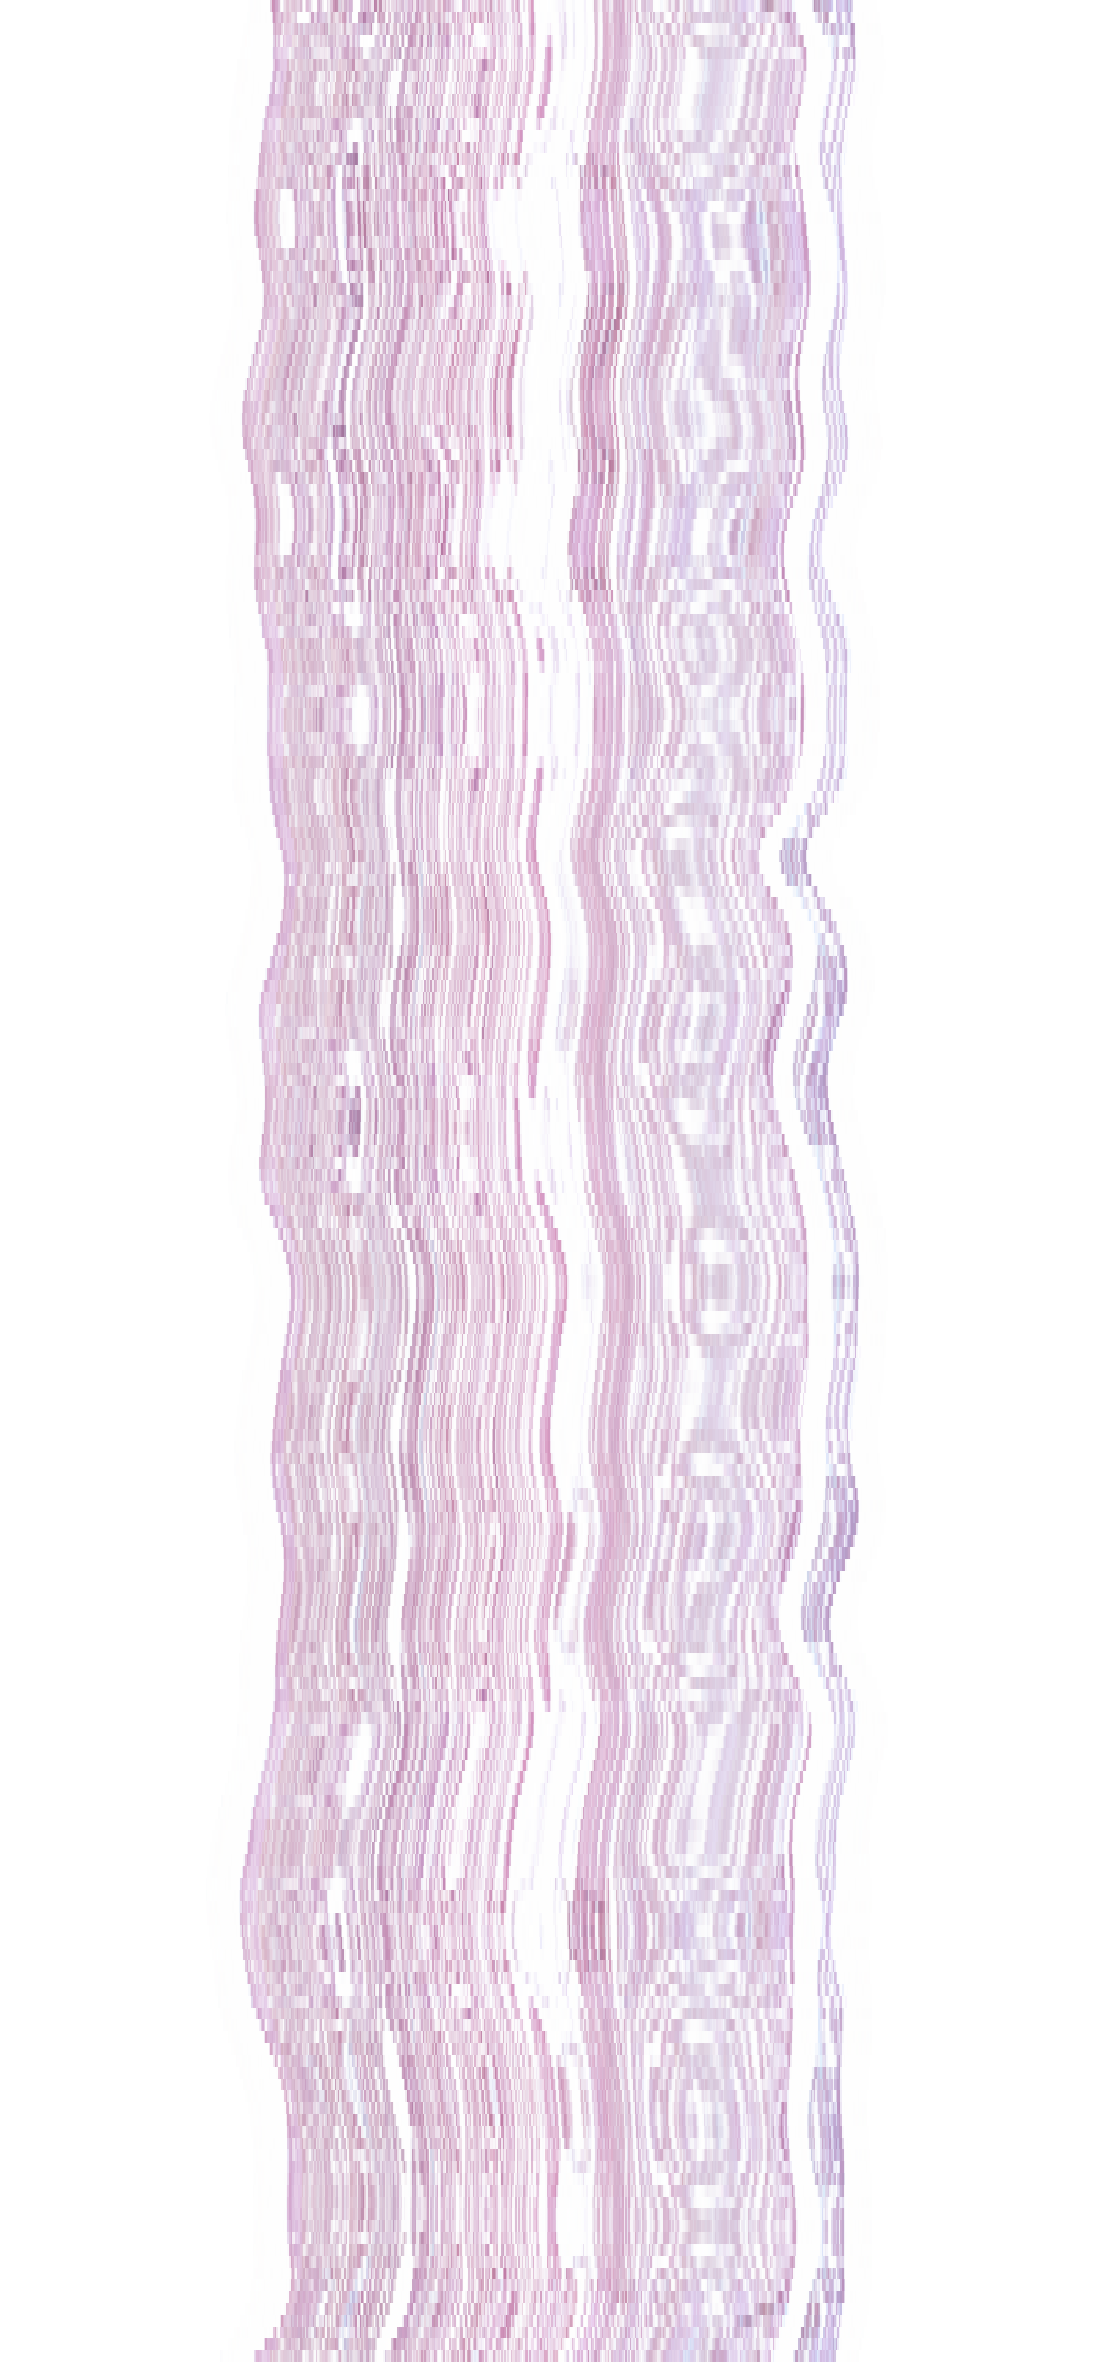
\includegraphics[height=0.4\textheight,type=pdf,ext=.pdf,read=.pdf]{Ch6/Figs/dummies/cross_section_200_alpha0.4_20_1_431}}
    \subfigure[][without noise]{\includegraphics[height=0.4\textheight,type=pdf,ext=.pdf,read=.pdf]{Ch6/Figs/dummies/cross_section_perfect_200_alpha0.4_1_431}}
    \caption{Cross-sections of the straight volume, perpendicular to the y-axis.}
    \label{fig:cross_section_1}
  \end{figure}
    
  % rotated
  \begin{figure}[htbp]
    \centering
    \subfigure[][0 iterations]{\includegraphics[height=0.4\textheight,type=pdf,ext=.pdf,read=.pdf]{Ch6/Figs/dummies/cross_section_200_alpha0.4r_0_0_352}}
    \subfigure[][1 iteration]{\includegraphics[height=0.4\textheight,type=pdf,ext=.pdf,read=.pdf]{Ch6/Figs/dummies/cross_section_200_alpha0.4r_1_0_352}}
    \subfigure[][3 iterations]{\includegraphics[height=0.4\textheight,type=pdf,ext=.pdf,read=.pdf]{Ch6/Figs/dummies/cross_section_200_alpha0.4r_3_0_352}}
    \subfigure[][8 iterations]{\includegraphics[height=0.4\textheight,type=pdf,ext=.pdf,read=.pdf]{Ch6/Figs/dummies/cross_section_200_alpha0.4r_8_0_352}}
    \subfigure[][20 iterations]{\includegraphics[height=0.4\textheight,type=pdf,ext=.pdf,read=.pdf]{Ch6/Figs/dummies/cross_section_200_alpha0.4r_20_0_352}}
    \subfigure[][without noise]{\includegraphics[height=0.4\textheight,type=pdf,ext=.pdf,read=.pdf]{Ch6/Figs/dummies/cross_section_perfect_200_alpha0.4r_0_352}}
    \caption{Cross-sections of the rotating volume, perpendicular to the x-axis.}
    \label{fig:cross_section_0r}
  \end{figure}
  
  \begin{figure}[htbp]
    \centering
    \subfigure[][0 iterations]{\includegraphics[height=0.4\textheight,type=pdf,ext=.pdf,read=.pdf]{Ch6/Figs/dummies/cross_section_200_alpha0.4r_0_1_431}}
    \subfigure[][1 iteration]{\includegraphics[height=0.4\textheight,type=pdf,ext=.pdf,read=.pdf]{Ch6/Figs/dummies/cross_section_200_alpha0.4r_1_1_431}}
    \subfigure[][3 iterations]{\includegraphics[height=0.4\textheight,type=pdf,ext=.pdf,read=.pdf]{Ch6/Figs/dummies/cross_section_200_alpha0.4r_3_1_431}}
    \subfigure[][8 iterations]{\includegraphics[height=0.4\textheight,type=pdf,ext=.pdf,read=.pdf]{Ch6/Figs/dummies/cross_section_200_alpha0.4r_8_1_431}}
    \subfigure[][20 iterations]{\includegraphics[height=0.4\textheight,type=pdf,ext=.pdf,read=.pdf]{Ch6/Figs/dummies/cross_section_200_alpha0.4r_20_1_431}}
    \subfigure[][without noise]{\includegraphics[height=0.4\textheight,type=pdf,ext=.pdf,read=.pdf]{Ch6/Figs/dummies/cross_section_perfect_200_alpha0.4r_1_431}}
    \caption{Cross-sections of the rotating volume, perpendicular to the y-axis.}
    \label{fig:cross_section_1r}
  \end{figure}
  
  % translated
  \begin{figure}[htbp]
    \centering
    \subfigure[][0 iterations]{\includegraphics[height=0.4\textheight,type=pdf,ext=.pdf,read=.pdf]{Ch6/Figs/dummies/cross_section_200_alpha0.4t_0_0_352}}
    \subfigure[][1 iteration]{\includegraphics[height=0.4\textheight,type=pdf,ext=.pdf,read=.pdf]{Ch6/Figs/dummies/cross_section_200_alpha0.4t_1_0_352}}
    \subfigure[][3 iterations]{\includegraphics[height=0.4\textheight,type=pdf,ext=.pdf,read=.pdf]{Ch6/Figs/dummies/cross_section_200_alpha0.4t_3_0_352}}
    \subfigure[][8 iterations]{\includegraphics[height=0.4\textheight,type=pdf,ext=.pdf,read=.pdf]{Ch6/Figs/dummies/cross_section_200_alpha0.4t_8_0_352}}
    \subfigure[][20 iterations]{\includegraphics[height=0.4\textheight,type=pdf,ext=.pdf,read=.pdf]{Ch6/Figs/dummies/cross_section_200_alpha0.4t_20_0_352}}
    \subfigure[][without noise]{\includegraphics[height=0.4\textheight,type=pdf,ext=.pdf,read=.pdf]{Ch6/Figs/dummies/cross_section_perfect_200_alpha0.4t_0_352}}
    \caption{Cross-sections of the translating volume, perpendicular to the x-axis.}
    \label{fig:cross_section_0t}
  \end{figure}
  
  \begin{figure}[htbp]
    \centering
    \subfigure[][0 iterations]{\includegraphics[height=0.4\textheight,type=pdf,ext=.pdf,read=.pdf]{Ch6/Figs/dummies/cross_section_200_alpha0.4t_0_1_431}}
    \subfigure[][1 iteration]{\includegraphics[height=0.4\textheight,type=pdf,ext=.pdf,read=.pdf]{Ch6/Figs/dummies/cross_section_200_alpha0.4t_1_1_431}}
    \subfigure[][3 iterations]{\includegraphics[height=0.4\textheight,type=pdf,ext=.pdf,read=.pdf]{Ch6/Figs/dummies/cross_section_200_alpha0.4t_3_1_431}}
    \subfigure[][8 iterations]{\includegraphics[height=0.4\textheight,type=pdf,ext=.pdf,read=.pdf]{Ch6/Figs/dummies/cross_section_200_alpha0.4t_8_1_431}}
    \subfigure[][20 iterations]{\includegraphics[height=0.4\textheight,type=pdf,ext=.pdf,read=.pdf]{Ch6/Figs/dummies/cross_section_200_alpha0.4t_20_1_431}}
    \subfigure[][without noise]{\includegraphics[height=0.4\textheight,type=pdf,ext=.pdf,read=.pdf]{Ch6/Figs/dummies/cross_section_perfect_200_alpha0.4t_1_431}}
    \caption{Cross-sections of the translating volume, perpendicular to the y-axis.}
    \label{fig:cross_section_1t}
  \end{figure}
    
  % rotated and translated
  \begin{figure}[htbp]
    \centering
    \subfigure[][0 iterations]{\includegraphics[height=0.4\textheight,type=pdf,ext=.pdf,read=.pdf]{Ch6/Figs/dummies/cross_section_200_alpha0.4rt_0_0_352}}
    \subfigure[][1 iteration]{\includegraphics[height=0.4\textheight,type=pdf,ext=.pdf,read=.pdf]{Ch6/Figs/dummies/cross_section_200_alpha0.4rt_1_0_352}}
    \subfigure[][3 iterations]{\includegraphics[height=0.4\textheight,type=pdf,ext=.pdf,read=.pdf]{Ch6/Figs/dummies/cross_section_200_alpha0.4rt_3_0_352}}
    \subfigure[][8 iterations]{\includegraphics[height=0.4\textheight,type=pdf,ext=.pdf,read=.pdf]{Ch6/Figs/dummies/cross_section_200_alpha0.4rt_8_0_352}}
    \subfigure[][20 iterations]{\includegraphics[height=0.4\textheight,type=pdf,ext=.pdf,read=.pdf]{Ch6/Figs/dummies/cross_section_200_alpha0.4rt_20_0_352}}
    \subfigure[][without noise]{\includegraphics[height=0.4\textheight,type=pdf,ext=.pdf,read=.pdf]{Ch6/Figs/dummies/cross_section_perfect_200_alpha0.4rt_0_352}}
    \caption{Cross-sections of the rotating and translating volume, perpendicular to the x-axis.}
    \label{fig:cross_section_0rt}
  \end{figure}
  
  \begin{figure}[htbp]
    \centering
    \subfigure[][0 iterations]{\includegraphics[height=0.4\textheight,type=pdf,ext=.pdf,read=.pdf]{Ch6/Figs/dummies/cross_section_200_alpha0.4rt_0_1_431}}
    \subfigure[][1 iteration]{\includegraphics[height=0.4\textheight,type=pdf,ext=.pdf,read=.pdf]{Ch6/Figs/dummies/cross_section_200_alpha0.4rt_1_1_431}}
    \subfigure[][3 iterations]{\includegraphics[height=0.4\textheight,type=pdf,ext=.pdf,read=.pdf]{Ch6/Figs/dummies/cross_section_200_alpha0.4rt_3_1_431}}
    \subfigure[][8 iterations]{\includegraphics[height=0.4\textheight,type=pdf,ext=.pdf,read=.pdf]{Ch6/Figs/dummies/cross_section_200_alpha0.4rt_8_1_431}}
    \subfigure[][20 iterations]{\includegraphics[height=0.4\textheight,type=pdf,ext=.pdf,read=.pdf]{Ch6/Figs/dummies/cross_section_200_alpha0.4rt_20_1_431}}
    \subfigure[][without noise]{\includegraphics[height=0.4\textheight,type=pdf,ext=.pdf,read=.pdf]{Ch6/Figs/dummies/cross_section_perfect_200_alpha0.4rt_1_431}}
    \caption{Cross-sections of the rotating and translating volume, perpendicular to the y-axis.}
    \label{fig:cross_section_1rt}
  \end{figure}
  
  The central cross-sections perpendicular to the x- and y-axes of the four regimes are exhibited in Figures~\labelcref{fig:cross_section_0,fig:cross_section_1,fig:cross_section_0r,fig:cross_section_1r,fig:cross_section_0t,fig:cross_section_1t,fig:cross_section_0rt,fig:cross_section_1rt}. The first section in each is of the original unsmoothed noisy volume, and the last of the volume before noise was added. Four images are sandwiched by these two extremes, of sections smoothed 1, 3, 8 and 20 times. The smoothing performs extremely well on two fronts. By iteration 20, a smooth, continuous section with the appearance of an original histology slice has been recovered from an unrecognisably noisy volume. Secondly and crucially, the underlying geometry of the tissue has been preserved, and the sections appear very similar to the ground truth sections before the noise had been added.
  
  % mean squared differences 3D
  \begin{sidewaysfigure}[htbp]
    \centering
    \subfigure[][straight column]{\includegraphics[height=0.33\textheight,type=pdf,ext=.pdf,read=.pdf]{Ch6/Figs/dummies/segmentation_mean_square_differences_3D}}
    \subfigure[][rotation]{\includegraphics[height=0.33\textheight,type=pdf,ext=.pdf,read=.pdf]{Ch6/Figs/dummies/segmentation_mean_square_differences_3Dr}}
    \subfigure[][translation]{\includegraphics[height=0.33\textheight,type=pdf,ext=.pdf,read=.pdf]{Ch6/Figs/dummies/segmentation_mean_square_differences_3Dt}}
    \subfigure[][rotation and translation]{\includegraphics[height=0.33\textheight,type=pdf,ext=.pdf,read=.pdf]{Ch6/Figs/dummies/segmentation_mean_square_differences_3Drt}}
    \caption{The 3D evolution of mean squared pixel intensity differences between adjacent slices for each of the four geometrical regimes.}
    \label{fig:mean_squared_differences_3D}
  \end{sidewaysfigure}
  
  Registration was performed using the mean square difference metric, and Figure~\ref{fig:mean_squared_differences_3D} graphs the evolving mean squared pixel intensity difference between each slice and its successor after repeated applications of the smoothing algorithm. In all four geometrical regimes, and for all slices away from the boundaries, the metric is greatly reduced, evidence that each slice is much more closely aligned with its neighbours. Just as in the case of 1D diffusion, most of the reduction is yielded in the earlier iterations, when the highest frequencies are damped most easily. Registrations were verified to be successful in the overwhelming majority of cases, ending with an oscillation around a consistent, very low mean squared difference value.
  
  % mean squared differences 2D
  \begin{sidewaysfigure}[htbp]
    \centering
    \subfigure[][straight column]{\includegraphics[height=0.33\textheight,type=pdf,ext=.pdf,read=.pdf]{Ch6/Figs/dummies/segmentation_mean_square_differences_2D}}
    \subfigure[][rotation]{\includegraphics[height=0.33\textheight,type=pdf,ext=.pdf,read=.pdf]{Ch6/Figs/dummies/segmentation_mean_square_differences_2Dr}}
    \subfigure[][translation]{\includegraphics[height=0.33\textheight,type=pdf,ext=.pdf,read=.pdf]{Ch6/Figs/dummies/segmentation_mean_square_differences_2Dt}}
    \subfigure[][rotation and translation]{\includegraphics[height=0.33\textheight,type=pdf,ext=.pdf,read=.pdf]{Ch6/Figs/dummies/segmentation_mean_square_differences_2Drt}}
    \caption{The initial (blue) and final (green) mean squared pixel intensities between adjacent pairs for each of the four geometrical regimes.}
    \label{fig:mean_squared_differences_2D}
  \end{sidewaysfigure}

  Figure~\ref{fig:mean_squared_differences_2D} graphs the initial and final metric values between adjacent pairs for the four test regimes. Note that each blue (resp. green) line is equivalent to the starting values on the left (resp. right) face of the corresponding plot in Figure~\ref{fig:mean_squared_differences_3D}. Almost ubiquitously, the value is substantially lower after transformational diffusion, with the green lines appearing much smoother after the high frequency spectrum has been preferentially damped.
  
  There is one notable example of a registration that has failed to reach a good alignment, manifested in Figure~\ref{fig:mean_squared_differences_3D}~\textbf{(a)} as a large spike in the metric value of slice 152 at iteration 6. The deviation is also visible in Figures~\labelcref{fig:cross_section_0,fig:cross_section_1}~\textbf{(d)} at iteration 8, as a large displacement two thirds of the way up from the base. At each iteration of the algorithm, the slices have moved relative to each other, and hence are initialised outside of any preceding local minimum trap. In this way, all adjacent slices are given multiple chances to become aligned, conferring to this method a great deal of robustness not present in any previous technique in the literature. By iteration 20 in Figures~\labelcref{fig:cross_section_0,fig:cross_section_1}~\textbf{(d)}, the aberration is imperceptible, and we can see from Figure~\ref{fig:mean_squared_differences_3D}~\textbf{(a)} that the erroneous metric value has returned to a level comparable with its neighbours after just four iterations.
  
  % full contours
  \begin{figure}[htbp]\texttt{}
    \centering
    \subfigure[][0 iterations]{\includegraphics[width=0.3\pagewidth]{Ch6/Figs/dummies/contours/whole_surface_0}}
    \subfigure[][1 iteration]{\includegraphics[width=0.3\pagewidth]{Ch6/Figs/dummies/contours/whole_surface_1}}
    \subfigure[][3 iterations]{\includegraphics[width=0.3\pagewidth]{Ch6/Figs/dummies/contours/whole_surface_3}}
    \subfigure[][8 iterations]{\includegraphics[width=0.3\pagewidth]{Ch6/Figs/dummies/contours/whole_surface_8}}
    \subfigure[][20 iterations]{\includegraphics[width=0.3\pagewidth]{Ch6/Figs/dummies/contours/whole_surface_20}}
    \caption{Isosurfaces of the perturbed straight volume in red at several stages of smoothing, overlayed with the unperturbed volume in green.}
    \label{fig:dummy_contour}
  \end{figure}
  
  \begin{figure}[htbp]
    \centering
    \subfigure[][0 iterations]{\includegraphics[width=0.3\pagewidth]{Ch6/Figs/dummies/contours/whole_surfacer_0}}
    \subfigure[][1 iteration]{\includegraphics[width=0.3\pagewidth]{Ch6/Figs/dummies/contours/whole_surfacer_1}}
    \subfigure[][3 iterations]{\includegraphics[width=0.3\pagewidth]{Ch6/Figs/dummies/contours/whole_surfacer_3}}
    \subfigure[][8 iterations]{\includegraphics[width=0.3\pagewidth]{Ch6/Figs/dummies/contours/whole_surfacer_8}}
    \subfigure[][20 iterations]{\includegraphics[width=0.3\pagewidth]{Ch6/Figs/dummies/contours/whole_surfacer_20}}
    \caption{Isosurfaces of the rotating volume.}
    \label{fig:dummy_contourr}
  \end{figure}
  
  \begin{figure}[htbp]
    \centering
    \subfigure[][0 iterations]{\includegraphics[width=0.3\pagewidth]{Ch6/Figs/dummies/contours/whole_surfacet_0}}
    \subfigure[][1 iteration]{\includegraphics[width=0.3\pagewidth]{Ch6/Figs/dummies/contours/whole_surfacet_1}}
    \subfigure[][3 iterations]{\includegraphics[width=0.3\pagewidth]{Ch6/Figs/dummies/contours/whole_surfacet_3}}
    \subfigure[][8 iterations]{\includegraphics[width=0.3\pagewidth]{Ch6/Figs/dummies/contours/whole_surfacet_8}}
    \subfigure[][20 iterations]{\includegraphics[width=0.3\pagewidth]{Ch6/Figs/dummies/contours/whole_surfacet_20}}
    \caption{Isosurfaces of the translating volumes.}
    \label{fig:dummy_contourt}
  \end{figure}
  
  \begin{figure}[htbp]
    \centering
    \subfigure[][0 iterations]{\includegraphics[width=0.3\pagewidth]{Ch6/Figs/dummies/contours/whole_surfacert_0}}
    \subfigure[][1 iteration]{\includegraphics[width=0.3\pagewidth]{Ch6/Figs/dummies/contours/whole_surfacert_1}}
    \subfigure[][3 iterations]{\includegraphics[width=0.3\pagewidth]{Ch6/Figs/dummies/contours/whole_surfacert_3}}
    \subfigure[][8 iterations]{\includegraphics[width=0.3\pagewidth]{Ch6/Figs/dummies/contours/whole_surfacert_8}}
    \subfigure[][20 iterations]{\includegraphics[width=0.3\pagewidth]{Ch6/Figs/dummies/contours/whole_surfacert_20}}
    \caption{Isosurfaces of the translating and rotating volumes.}
    \label{fig:dummy_contourrt}
  \end{figure}
  
  The nature of the 3D geometry of the volumes --- the rotation and translation signals, and the transformational noise --- is most clearly understood from the segmentation volume isosurfaces in Figures~\labelcref{fig:dummy_contour,fig:dummy_contourr,fig:dummy_contourt,fig:dummy_contourrt}. Each of the 5 levels of smoothing depicted by Figures~\labelcref{fig:cross_section_0,fig:cross_section_1,fig:cross_section_0r,fig:cross_section_1r,fig:cross_section_0t,fig:cross_section_1t,fig:cross_section_0rt,fig:cross_section_1rt} are overlayed in red with their equivalent unperturbed volumes in green. Again, the smoothing brings the noisy volume much more closely in line with the ground truth, with the largest effect on the higher frequencies of noise. The conservation of the underlying structure is most evident in Figure~\ref{fig:dummy_contourrt}~(e), where the red isosurface deviates almost imperceptibly from the green.
  
  Parameters used in the registration are listed in Table~\ref{tab:dummy_histo_to_histo}. It is worth noting that as long as the registration process is refined enough to arrive dependably near the global minimum, the adjustment algorithm itself is stable with much larger levels of noise than showcased here. For example, one approach might be to preprocess images and tune parameters to cope with large displacements for the first few smoothing iterations, and then tune for smaller displacements during the finer smoothing in the later iterations. Yet, this kind of approach requires heavy manual intervention, and is highly specific to the problem at hand.
  % subsection simulating_transformational_diffusion (end)
% section methods (end)

\section{Results} % (fold)
\label{sec:results}
  \subsection{Global Diffusion} % (fold)
  \label{sub:global_diffusion}
    % x slices
    \begin{figure}[htbp]
      \centering
      \subfigure[][0 iterations (unsmoothed affine volume)]{\includegraphics[height=0.31\textheight]{Ch6/Figs/adjusted_0_0_235}}
      \subfigure[][1 iteration]{\includegraphics[height=0.31\textheight]{Ch6/Figs/adjusted_1_0_235}}
      \subfigure[][20 iterations]{\includegraphics[height=0.31\textheight]{Ch6/Figs/adjusted_20_0_235}}
      \caption{Cross-sections of the full Rat28 volume perpendicular to the x-axis, after 0, 1 and 20 iterations of diffusion. The yellow boxes highlight the zoomed regions in Figure~\ref{fig:adjusted_bottom_vessels_0_235}.}
      \label{fig:adjusted_0_235}
    \end{figure}

    % y slices
    \begin{figure}[htbp]
      \centering
      \subfigure[][0 iterations (unsmoothed affine volume)]{\includegraphics[height=0.31\textheight]{Ch6/Figs/adjusted_0_1_287}}
      \subfigure[][1 iteration]{\includegraphics[height=0.31\textheight]{Ch6/Figs/adjusted_1_1_287}}
      \subfigure[][20 iterations]{\includegraphics[height=0.31\textheight]{Ch6/Figs/adjusted_20_1_287}}
      \caption{Cross-sections of the full Rat28 volume perpendicular to the y-axis, after 0, 1 and 20 iterations of diffusion. The yellow boxes highlight the zoomed regions in Figure~\ref{fig:adjusted_bottom_vessels_1_287}.}
      \label{fig:adjusted_1_287}
    \end{figure}
    
    20 iterations of smoothing were applied to the affine registered full-heart volume from Section~\ref{sec:registration_results}, and Figures~\labelcref{fig:adjusted_0_235,fig:adjusted_1_287} compare the central cross-sections of the volume before smoothing, after 1 iteration and after all 20 iterations. A subtle, but unmistakable improvement in coherence is observed; internal and external edges are smoother, especially towards the extremities of the heart, and clear, waving sheet structure has emerged, previously indistinguishable beyond the high-frequency zig-zagging noise.
    
    % lower 100 slices zoom
    % x slices
    \begin{sidewaysfigure}[htbp]
      \centering
      \subfigure[][0 iterations (unsmoothed affine volume)]{\includegraphics[height=0.12\textheight]{Ch6/Figs/adjusted_0_0_235_zoomed}}
      \subfigure[][1 iteration]{\includegraphics[height=0.12\textheight]{Ch6/Figs/adjusted_1_0_235_zoomed}}
      \subfigure[][20 iterations]{\includegraphics[height=0.12\textheight]{Ch6/Figs/adjusted_20_0_235_zoomed}}
      \caption{Cross-sections of the lower 100 slices perpendicular to the x-axis. The blue arrows highlight blue-stained interstitial tissue around vessels, the green arrow epicardial vessels and the yellow arrow enhanced sheet structure.}
      \label{fig:adjusted_bottom_vessels_0_235}
    \end{sidewaysfigure}

    % y slices
    \begin{sidewaysfigure}[htbp]
      \centering
      \subfigure[][0 iterations (unsmoothed affine volume)]{\includegraphics[height=0.12\textheight]{Ch6/Figs/adjusted_0_1_287_zoomed}}
      \subfigure[][1 iteration]{\includegraphics[height=0.12\textheight]{Ch6/Figs/adjusted_1_1_287_zoomed}}
      \subfigure[][20 iterations]{\includegraphics[height=0.12\textheight]{Ch6/Figs/adjusted_20_1_287_zoomed}}
      \caption{Cross-sections of the lower 100 slices perpendicular to the y-axis. The green arrows highlight epicardial vessels and the yellow arrow enhanced sheet structure.}
      \label{fig:adjusted_bottom_vessels_1_287}
    \end{sidewaysfigure}
    
    The effect is clearer in an enlargement of the bottom 100 slices in Figures~\labelcref{fig:adjusted_bottom_vessels_0_235,fig:adjusted_bottom_vessels_1_287}. The outer walls are several orders of magnitude less noisy in both figures, and internal vessel walls are much more coherent, most notably the epicardial vessels on the left and right of Figure~\ref{fig:adjusted_bottom_vessels_1_287}~(c). Sheet structure that started to surface from obscurity after just one iteration has been well resolved after 20 iterations. Figures~\labelcref{fig:whole_positive_x_diffused,fig:whole_negative_x_diffused,fig:whole_positive_y_diffused,fig:whole_positive_z_diffused} depict the smoother global contour after 20 iterations from several angles.
    
    % diffused contours
    \begin{sidewaysfigure}[p]
      \centering
      \includegraphics[width=0.9\textheight]{Ch6/Figs/Rat28/contours/whole_positive_x_diffused}
      \caption{Globally smoothed slice volume, viewed along the positive x direction.}
      \label{fig:whole_positive_x_diffused}
    \end{sidewaysfigure}

    \begin{sidewaysfigure}[p]
      \centering
      \includegraphics[width=0.9\textheight]{Ch6/Figs/Rat28/contours/whole_positive_z_diffused}
      \caption{Globally smoothed slice volume, viewed along the positive z direction.}
      \label{fig:whole_positive_z_diffused}
    \end{sidewaysfigure}
  % subsection global_diffusion (end)
  
  \subsection{Regional Diffusion} % (fold)
  \label{sub:regional_diffusion}
    \begin{figure}[p]
      \centering
      \subfigure[][Original block face registration]{\includegraphics[height=0.21\textheight]{Ch6/Figs/bottom_vessels/unsmoothed_vessel_0_2875}}
      \subfigure[][Globally smoothed registration]{\includegraphics[height=0.21\textheight]{Ch6/Figs/bottom_vessels/globally_smoothed_vessel_0_2875}}
      \subfigure[][Regionally smoothed registration]{\includegraphics[height=0.21\textheight]{Ch6/Figs/bottom_vessels/regionally_smoothed_vessel_0_2875}}
      \caption{Central cross sections of the region around an epicardial vessel, perpendicular to the x axis. Cross-sections are compared before smoothing, after global smoothing and after smoothing applied to this region. The blue arrow highlights blue-stained interstitial tissue around vessels, the green arrow epicardial vessels and the yellow arrow enhanced sheet structure.}
      \label{fig:vessel_cross_section_x}
    \end{figure}
    
    \begin{figure}[p]
      \centering
      \subfigure[][Original block face registration]{\includegraphics[height=0.21\textheight]{Ch6/Figs/bottom_vessels/unsmoothed_vessel_1_2125}}
      \subfigure[][Globally smoothed registration]{\includegraphics[height=0.21\textheight]{Ch6/Figs/bottom_vessels/globally_smoothed_vessel_1_2125}}
      \subfigure[][Regionally smoothed registration]{\includegraphics[height=0.21\textheight]{Ch6/Figs/bottom_vessels/regionally_smoothed_vessel_1_2125}}
      \caption{Central cross sections of the region around an epicardial vessel, perpendicular to the y axis.  The blue arrow highlights blue-stained interstitial tissue around vessels, the green arrow epicardial vessels and the yellow arrow enhanced sheet structure.}
      \label{fig:vessel_cross_section_y}
    \end{figure}
    
    \begin{sidewaysfigure}[p]
      \centering
      \includegraphics[width=\textwidth]{Ch6/Figs/bottom_vessels/regionally_smoothed_vessel_2_046}
      \caption{Full resolution image of the central slice of the epicardial vessel region. The yellow box represents the bounds of Figure~\ref{fig:cropped_vessel_cross_section_z}.}
      \label{fig:vessel_cross_section_z}
    \end{sidewaysfigure}
    
    \begin{figure}[p]
      \centering
      \includegraphics[width=\textwidth]{Ch6/Figs/bottom_vessels/cropped_regionally_smoothed_vessel_2_046}
      \caption{A zoomed 200$\mu$m by 200$\mu$m square of full resolution image of the geometric centre of Figure~\ref{fig:vessel_cross_section_z}.}
      \label{fig:cropped_vessel_cross_section_z}
    \end{figure}
    
    A regional registration around an epicardial vessel yields even further improvement, when at this smaller scale, curvature and distortions not represented by an affine transformation become less significant. The final transforms from the global smoothings were used to initialise the regional smoothings, with the centre of transformation moved to the geometric centre of the region. In order to smooth the cost function adequately for the optimiser, the images used to perform the registration were Gaussian smoothed and downsampled by a factor of 8: a level optimal to resolve features the size of an epicardial vessel. Figures~\labelcref{fig:vessel_cross_section_x,fig:vessel_cross_section_y} show two central perpendicular cross-sections of the epicardial region before smoothing, after global smoothing and after an additional regional smoothing. Figures~\labelcref{fig:vessel_cross_section_z,fig:cropped_vessel_cross_section_z} remind us of the order-of-magnitude greater resolution in plane (1.1$\mu$m) with respect to the vertical out-of-plane resolution (10$\mu$m) in Figures~\labelcref{fig:vessel_cross_section_x,fig:vessel_cross_section_y}, displaying the central slice of the region at full resolution.
    
    \begin{figure}[p]
      \centering
      \subfigure[][Unsmoothed segmentation]{\includegraphics[width=0.7\textwidth]{Ch6/Figs/bottom_vessels/unsmoothed_segmentation}}
      \subfigure[][Globally smoothed segmentation]{\includegraphics[width=0.7\textwidth]{Ch6/Figs/bottom_vessels/globally_smoothed_segmentation}}
      \subfigure[][Locally smoothed segmentation]{\includegraphics[width=0.7\textwidth]{Ch6/Figs/bottom_vessels/locally_smoothed_segmentation}}
      \caption{Surface contours of segmentations of vasculature (red) and epicardium (green) in the region around an epicardial vessel from Figures~\labelcref{fig:vessel_cross_section_x,fig:vessel_cross_section_y,fig:vessel_cross_section_z,fig:cropped_vessel_cross_section_z}, from the unsmoothed, globally smoothed and locally smoothed volumes.}
      \label{fig:region_segmentations}
    \end{figure}
    
     A confidence connected component segmentation was employed to generate the segmentations in Figure~\ref{fig:region_segmentations}, which, unlike methods such as level set segmentation or neighbourhood filters, does not introduce any artificial surface smoothing. Progressive enhancement in coherence is visible from the back cross-section, the vessel surface and the pericardial surface, from (a) to (b) and then to (c); the contours in (c) are almost totally smooth, with only the inherent stepping of each individual histology slice visible. In particular, the disturbance near the top of the largest vessel in (b) has been smoothed in (c). Original adjacent slice aberrations in (a) reached ~450$\mu$m. Contrastingly in (c), the relative registration error is reduced below the diameter of even the smallest vessels, by inspection less than 5$\mu$m in the large majority of cases - smaller than the width of a single myocyte. Resultingly, with each of the two smoothing procedures, more of the smaller vasculature has become connected to the main vessel and has been segmented.
    
    \begin{sidewaysfigure}[p]
      \centering
      \includegraphics[width=0.9\textwidth]{Ch6/Figs/bottom_vessels/vessel_overlay}
      \caption{An overlay of the three vessel segmentations from Figure~\ref{fig:region_segmentations}. The unsmoothed vessel is shaded in red, the globally smoothed vessel in amber and the regionally smoothed vessel in green. }
      \label{fig:vessel_segmentations}
    \end{sidewaysfigure}
    
    We see the combined results of all three vascular segmentations in Figure~\ref{fig:vessel_segmentations}. From this view through the pericardium, the striking continuity of the green surface is most apparent. The overall shape of the green vessel precisely intersects the disconnected set of red discs, demonstrating that the underlying vessel geometry has been recovered with remarkable accuracy. Again it is clear that the reduction in error below the diameter of the smallest vessels has facilitated their segmentation, with several thin green dendritic structures reaching up into the top left of the figure.
  % subsection regional_diffusion (end)

% section results (end)

\section{Discussion} % (fold)
\label{sec:discussion}
  We have invented a robust and mathematically elegant method of resolving volumes from noisy 2-dimensional image slices, transferring transformational information between neighbouring slices. It excels any current technique in the literature at providing smooth, continuous volumes, whilst preserving underlying geometry. Further, its iterative nature confers to it a resilience to the trap of local minima, to registration failures and to outliers, which is unmatched by contemporary methods; even when the cost function of a registration is spiky, and results of a single run are sensitive to initialisation, the diffusion algorithm provides multiple opportunities to escape local basins in the cost function, having shifted the cost landscape each time. Contrastingly in the case of banana registration, the displacement from one unsuccessful registration is propagated to \emph{every} subsequent slice in the volume.
  
  One might reasonably consider, as an alternative implementation, the registration of more than just the nearest neighbours at each iteration, but the \emph{k}-nearest neighbours, followed by the application of some (binomial) weighted mean of the results:
  
  \begin{equation}
    \mathbf{\Delta T}_i^{n,n+1} = \sum_{j=-k}^k \binom{2k}{j+k}\alpha \cdot \mathbf{\Delta T}_{i,i+j}^n,
  \end{equation}
  
  where we define the sum operator $\sum$ as
  
  \begin{equation}
    \sum_{i=0}^n \mathbf{T}_i = \mathbf{T}_0 \oplus \mathbf{T}_1 \oplus \ldots \oplus \mathbf{T}_n.
  \end{equation}
  
  Indeed, in 1-dimensional diffusion, $n$ iterations of nearest neighbour diffusion (where $k=1$) is equivalent to a single binomial iteration across a larger neighbourhood ($k=n$). There are three reasons why this approach is suboptimal. Firstly, inaccurate or erroneous registrations --- most likely to occur in the earliest stages with the most noise --- are given fewer chances to be mitigated by later iterations. Equivalently from another perspective, more registrations are performed under higher levels of perturbation than necessary. Secondly, the further away two histological slices are from each other within the real tissue volume, the more different they appear, and thus a successful registration between them is less likely. Thirdly, no computational time is saved, as the same total number of slice-to-slice registrations must be performed for a given level of smoothing. In fact, total computation is likely to be extended, as the more challenging registrations that are introduced will take longer to reach an optimum.
  
  As was mentioned at the end of Section~\ref{ssub:formulating_the_transform_operators}, this diffusion technique could be extended easily to more complex transforms, as long as that set of transformations form a Lie group. Diffeomorphic transformations fall under this category, and their differentiable and invertible properties are exploited to similar ends in the literature \cite{Avants2006}. Consistent B-splines may also be constrained to be quasi-invertible \cite{Arganda-Carreras2010}. Many transforms commonly used in registration, such as b-spline and other piecewise transforms, are excluded from this classification. In practice, the markedly lax constraint for improvement --- that the algorithm must simply  move each slice somewhat closer to its neighbours --- coupled with the fact that all transforms approximate a Lie group in the small limit, mean that a trivial linear interpolation of any transform's parameters will lead to reliable and geometrically faithful smoothing for noise levels significantly smaller than the scale of the registration.
    
  One of the main decisions when enhancing volumes with diffusion smoothing is how many iterations should be applied. If the amplitude of the noise frequency spectrum is distributed higher and away from the true underlying geometrical spectrum, then after an initial few iterations of successful noise reduction, the volume will remain largely unchanged in a wide optimal window, whilst a basin of near-zero amplitude frequencies are being damped. Eventually of course, the true low-frequency signal will begin damping, leading to undesired banana-like effects. In practice, it is often simple to detect this window by comparing the output volumes of a range of iteration numbers, looking for the smallest changes in the appearance of cross-sections or segmented contours.
  
  Choosing the optimal number of iterations becomes more complex when preserving genuinely acute image curvature. Just as in the case of 1-dimensional diffusion, true underlying high-frequency signal will be smoothed indiscriminately along with noise. For example, any sharp variation in the cardiac geometry of Section~\ref{sub:regional_diffusion} expressed across fewer than $\sim$5 slices will be smoothed significantly after 20 iterations. Where the banana problem erroneously symmetrises a geometry, diffusion smoothing can erroneously symmetrise the \emph{curvature} of a geometry, if applied too heavily. Anisotropic diffusion based either upon some scalar measure of the magnitude of the transforms between slices, or upon the images or pairs of images themselves, could well be employed to dampen the diffusive coefficient $\alpha$ adaptively, in regions of strong variation where curvature must be preserved. Anisotropic diffusion is used widely in order to clear up noise in the intensity of images, and ~\cite{Arsigny2005} apply anisotropic diffusion to tensor images through a log-Euclidian framework.
  
  Even though the algorithm is robust to the occasional erroneous registration, nothing can make up for a consistent failure to coregister a pair of slices toward each other. In some specific cases, such as a hypothetical straight featureless section of myocardium, the degenerate shapes of slice pairs lead to a flat cost function basin parallel to the myocardial wall, which stifles true matching. Nevertheless, in many cases, careful tuning based on observations of metric value evolution and progress volumes using the tools developed in Section~\ref{sub:diagnostics} can yield a parameter set suitable across all the slice pairs of the volume. Indeed, when registering adjacent slices in the region in Section~\ref{sub:regional_diffusion}, the moving slice pericardium was observed to gravitate quickly and directly towards that of the fixed slice. A slower alignment parallel to the epicardial wall then followed, owing to the displaced but overlapping white epicardial vessel discs, such as in Figure~\ref{fig:vessel_cross_section_z}. In general, image features larger than the maximum amplitude of noise can provide monotonic paths through parameter space to the global minimum.
  
  Boundary conditions at edge slices should be chosen based upon the error in the the edge slice positioning, and upon an estimate of the symmetry at the boundary. Where the error in the edge slice position is thought to be larger than the transformational gradient near the boundary, zero-Neumann discrete boundary conditions can be implemented; a ghost slice that perfectly matches the edge slice with the identity transform is used, along with its single neighbour, to calculate its diffusion at each iteration. This of course introduces banana-like straightening effects near the boundary, as the influx of contributions from the identity penetrate the volume. Alternatively, if the gradient of transformation can be estimated near the boundary, for example via the inverse transforms of the banana registration of the reference images, then non-zero Neumann conditions should be used. Where the positions of boundary slices are considered accurate, Dirichlet-like boundary conditions can lock them in place. Of course, if appropriate, a combination of Neumann and Dirichlet boundary conditions can be implemented.
  
  Going forward, log-Euclidean statistics could be used for averaging pair-wise registrations between 3D data sets, for example between a set of rat hearts. A single representative map could then be developed from the whole dataset, and statistics such as anatomical variation extracted from it. The diffusion framework could also be used to smooth out jolting or high-frequency transformational noise in 4D time-series datasets, whilst maintaining the overall positioning of features in space.
  
  Now that we have constructed a smooth, continuous 3D image of cardiac tissue, it remains to extract anatomical information from this volume, with a view to building anatomically-based models for simulation. In the next chapter, we explore the feasibility of such a development.
% section discussion (end)

% chapter diffusion_smoothing_registration_of_high_resolution_rat_histology (end)


%%%%%%%%%%%%%%%%%%%%%%%%%%%%%%%%%%%%%%%%%%%%%%%%%%
%
\def\localpath{Ch7}
\chapter{2D and 3D Analysis of Fibre and Sheet Orientation}
% If you like chapter abstracts ...
\dblspace
\begin{quote}{\em %!TEX root = ../thesis.tex

In this chapter, we develop quantitative methods to discern orientation information from 2D and 3D images, based on what is known as the structure tensor. We validate the methods on a single 2D region of left-ventricular myocardial wall and demonstrate that, given images of the required detail and coherence, orientation at a range of scales can be inferred with a high degree of accuracy. We extract volumetric image gradients from the reconstructed images in Chapter~\ref{cha:diffusion_smoothing_registration_of_high_resolution_rat_histology}, in the hope that these gradients will correlate closely with the local myocardial fibre direction. We establish that in this case, even extremely small registrational abberations lead to large artificial increases in intensity gradients perpendicular to the histological plane, hindering the faithful extraction of fibre direction for inclusion in models for electrophysiological simulation.
}\end{quote}
%!TEX root = ../thesis.tex
\chapter{Coregistration of High Resolution Rat Histology}
% If you like chapter abstracts ...
\dblspace
\begin{quote}{\em %!TEX root = ../thesis.tex
Adjacent histological slices can be coregistered accurately and lead to smooth image volumes, owing to their close morphological resemblance and their similar intensity spectra. However, volumes constructed from serial histology registration do not reflect the true 3-dimensional tissue geometry. Registration of histology to a set of coherent reference images yields an authentic geometry on the organ scale, yet the lower resolution and differing modality of the references leads to noisy, jagged volumes on the microstructural scale.

We present in this chapter an algorithm to align neigbouring slices accurately and smoothly without disturbing large scale tissue shape, based on a microscopic model of diffusion. We develop a mathematically sound and general framework of transformational diffusion, based on the Lie theory of continous groups. Using synthetic geometries of cardiac tissue with artificial noise, we demonstrate a robust and precise dispersion of information between slices on a configurable range of scales, recovering volumes which are orders of magnitude smoother and which have maintained faithfully the underlying geometrical signal. We apply the algorithm to the volumes from Chapter~\ref{cha:coregistration_of_high_resolution_rat_histology}, first globally and then again to the region around an epicardial vessel. Previously indiscernible microvasculature and sheet structure becomes patent. Pericardium and epicardial vessel segmentations show that displacement abberations between adjacent slices of the order of 400$\mu$m are reduced by two orders of magnitude. The methods presented here outperform any such method to reconstruct histological volumes based on reference images currently in the literature. Finally, we discuss several interesting applications and refinements that might be made to the algorithm in specific cases, including anisotropic diffusion based on image features or inter-slice transform magnitudes.

}\end{quote}







%%%%%%%%%%%%%%%%%%%%%%%%%%%%%%%%%%%%%%%%%%%%%%%%%%
%
\def\localpath{Ch8}
\chapter{The Role of Cardiac Microstructure in Propagation Dynamics}
% If you like chapter abstracts ...
\dblspace
\begin{quote}{\em \input{Ch8/abstract8}}\end{quote}
%!TEX root = ../thesis.tex
\chapter{The Role of Cardiac Microstructure in Propagation Dynamics}
% If you like chapter abstracts ...
\dblspace
\begin{quote}{\em \input{Ch8/abstract8}}\end{quote}

\section{Introduction}
\label{sec:review:introduction}
CONFIRMATION THESIS
The previous chapter characterises the geometrical differences between DTMRI and detailed histology. This chapter aims to quantify the functional consequences of incorporating this detail into models, by simulating propagation and arrhythmias on geometries derived from the two modalities, in regions where they differ significantly. Specifically, plane wave propagation and triggered arrhythmias will be simulated over the papillary muscle insertion, the apex, epicardial arteries and the junction of the septum and the free wall.

We examine the hypothesis that heterogeneity such as rapidly varying or discontinuous fibre orientation, tissue type boundaries and non-conducting artefacts such as epicardial arteries act to promote wave curvature and stabilise arrhythmia, based on the findings from the simulations. We quantify the orthotropic effects of sheet structure. We design stimulation protocols and simulation regimes for each region. We run simulations in Chaste. We analyse the lifetimes of reentrant waves, the numbers and interactions of singularity filaments, and the anchoring effect of heterogeneities on filaments. We then run simulations on DTMRI-derived models of the same regions and compare the findings with our previous results, to illuminate whether the detail provided by the histology is important, or whether the noise in the DTI data is significant.
CONFIRMATION THESIS

PAPER OUTLINE FROM CONFIRMATION THESIS
\subsection{The Role of Cardiac Microstructure in Propagation Dynamics: A Modelling and Simulation Study}
\subsubsection{Aims and Hypotheses}
The previous paper accurately exposed cardiac microstructural geometries, and stood this new information in contrast with geometries obtained from DTMRI data. The main aim of this paper is to characterise the functional consequences of incorporating this detail into models, by simulating arrhythmias in regions of interest, and comparing the findings with analogous simulations based on DTI data. The wider hypothesis, that the inclusion of detail in highly heterogeneous zones promotes wave curvature and breakup and fosters arrhythmia, can be broken down into the following proposals:
\begin{itemize}
  \item Sharp discontinuities are present at the papillary insertions and the junction of the septum with the myocardial free wall. Incoherent, crossing fibre directions are observed around the apex of the heart. We propose that rapidly varying fibre direction in these regions promotes wave curvature and helps sustain arrhythmia.
  \item Leading on from observations in paper 2, we propose that in the region of epicardial arteries, the anchoring effect is mitigated by the insulating tissue on the outside of epicardial arteries, when compared to simulations on the same geometries modelled solely as myocardium.
  \item \emph{Possibly? We propose that the non-conducting interstitial spaces that divide the myocardium into sheets engender orthotropic conductivity on a macroscopic scale.}
\end{itemize}

\subsubsection{Methods}
\paragraph{Models}
Four types of model will be used: those based solely on histology; those based on registered and segmented DTMRI; those with histological segmented geometry, but with DTMRI-derived fibre orientations; and those with DTMRI geometries and rule-based fibre orientations.

\paragraph{Simulation}
  Similar protocols to those employed in the first simulation paper will serve on the image-based models. Single stimulation protocols can elucidate the effect of microstructure on wavefront curvature during normal cardiac function. Double stimulation protocols will initiate arrhythmia in ROIs, and times until cessation will be compared between the smooth and the accurate geometries.
  
\subsubsection{Results}
Each hypothesis will be scrutinised in light of the results. Phase singularity filaments will be analysed in terms of their numbers, interactions, breakups and lifetimes.

\subsubsection{Discussion and Conclusions}
The functional importance of the inclusion of microstructure in models for simulation will be made clear by the results.
PAPER OUTLINE FROM CONFIRMATION THESIS

% Appendices %%%%%%%%%%%%%%%%%%%%%%%%%%%%%%%%%%%%%
\appendix
\dblspace
%
\chapter{Dull stuff in the Appendix}
\def\localpath{ApA}

This appendix is about

\section{My first section}
\label{sec:detail:myfirst}

\section{Conclusions}
\label{sec:detail:conclusions}

Smurfle gibber. Ain't it good.


\sglspace

%%%%%%%%%%%%%%%%%%%%%%%%%%%%%%%%%%%%%%%%%%%%%%%%%%
% Bibstuff
\pagestyle{bibheadings}

\bibliographystyle{Setup/JRSS_no_url}   % For just numbers
%\bibliographystyle{alpha}   % For initials+year
%\bibliographystyle{apalike} % For full surname
\bibliography{refs}

\end{document}
